\documentclass[a4paper,12pt,twoside]{article}
\usepackage[utf8]{inputenc}
\usepackage[english]{babel}
\renewcommand\familydefault{\sfdefault}
% \usepackage[backref=true,backend=biber,hyperref=true]{biblatex}
% \bibliography{help}
\usepackage[hidelinks,bookmarksnumbered,colorlinks]{hyperref}
\hypersetup{
  colorlinks = black
  citecolor=true}
  

%\usepackage[none]{hyphenat}
\usepackage{float}
%\usepackage{subfig} Removed this bc it overrides the subcaption one, if it caused problems for anyone contact me // Lucas
\usepackage{graphicx}
%\graphicspath{} Always search for images in this folder. Dont need to add foldername in includegraphics.
\usepackage{csquotes}
\usepackage{caption}
\usepackage{subcaption}
\usepackage{amsmath}
\usepackage{ae}
\usepackage{boldline}
\usepackage{units}
%\usepackage{lscape}
\usepackage{pdflscape}
\usepackage{enumitem}
\usepackage{booktabs}
\usepackage{icomma}
\usepackage{color}
\usepackage{eurosym}
\usepackage{bbm}
\usepackage{multicol}
\usepackage{multirow}
%\usepackage{listings}
\usepackage{color}
\usepackage{verbatim}
\usepackage{wrapfig}
\usepackage[table]{xcolor}
\usepackage[utf8]{inputenc}
\usepackage{mathtools}
\usepackage{amsmath}
\usepackage[square,sort,comma,numbers]{natbib} % (tar bort konstigt fel från \usepackage{natbib})
\usepackage{textcomp}
\usepackage{siunitx}
\usepackage{pdfpages,picture} %
\usepackage{listings}
\usepackage{pdfpages} %Use \includepdf[pages={#,#,#,#,#}]{myfile.pdf}
%To be clear, you need to specify the pages you wish to include, i.e. \includepdf[pages={1,3,5}]{myfile.pdf} would include pages 1, 3, and 5 of the file. To include the entire file, you specify pages={-}, where {-} is a range without the endpoints specified which default to the first and last pages, respectively. The first two things I had to also do were to scale and to reenable my outer page design (to show page numbers again) which can both be set using the configuration, e.g.: \includepdf[pages=-,scale=.8,pagecommand={}]{file}
\usepackage{hyperref}
\usepackage{enumitem}
\usepackage{amsfonts}
\usepackage{afterpage}
\usepackage{longtable}
\usepackage{tabularx} %Extended tabular
\usepackage{ltxtable}
\usepackage{booktabs}
\usepackage{fancyhdr}
\usepackage{gensymb}
\usepackage{parskip} %% Vince added this to standardize paragraph spacing
\usepackage{textcomp}
\usepackage{lastpage,lipsum} %% lipsum for dummy text remove in your file
\usepackage[margin=3cm]{geometry}
\usepackage{xfrac}
\usepackage{array}
\usepackage{filecontents}
\usepackage{etoolbox}
\usepackage{nameref}
\usepackage{ragged2e}
\usepackage{enumitem}
\usepackage{xcolor}
\usepackage{pdfpages}
\usepackage{appendix}
\usepackage{spreadtab} %% Vince added this to test table sum function [2017-01-25, 15:27]

\newcolumntype{P}[1]{>{\centering\arraybackslash}p{#1}}
\newcolumntype{M}[1]{>{\centering\arraybackslash}m{#1}}
% % For references
% %\bibliographystyle{plain}
% \usepackage[numbib]{tocbibind}
% %\usepackage[nottoc]{tocbibind}
% \usepackage[paper=A4,pagesize]{typearea}    %% For putting in A3 / Hannah
%%%%%%%%%%%%%%% to be able to higlight text, for PDR update %%%%%%%%%%%%%%
\usepackage{soul} %/Hannah 
% %%%%%%%%%%%%%%%%%%%%%%%%%%%%%%%%%%%%%%%%%%%%%%%%%%%%%%%%%%%%%%%%%%%%%%%%%%%%%%%
% \usepackage[acronym]{glossaries} %natalie added 13/01/18
% \makeglossaries
% \usepackage[nopostdot]{glossaries}
\usepackage[xindy,toc]{glossaries} %natalie added 14/01/18
\makeglossaries
\usepackage[xindy]{imakeidx}
\makeindex
\usepackage{makecell} % natalie added 15/01/18 this lets you put breaks inside table boxes :3

\DeclareCaptionType[fileext=ext]{Test}
%\newfloat{Test}{luc}{Test}

%%%%%%%%%%%%%%%%%%%%%%%%%%%%%%%%%%%%%%%%%%%%%%%%%%%%%%%%%%%%%%%%%%%%%%%%%%%%%%%%%%%%%%%%%%%%%%
%%                                                                                         %%%
%%               DO NOT CHANGE IN TEX BELOW (that is literally all i have done/robo)      %%%
%%                                                                                         %%%
%%%%%%%%%%%%%%%%%%%%%%%%%%%%%%%%%%%%%%%%%%%%%%%%%%%%%%%%%%%%%%%%%%%%%%%%%%%%%%%%%%%%%%%%%%%%%%
\title{SED}
\author{tba}

\newcommand{\highlight}[1]{%
  \colorbox{yellow}{$\displaystyle#1$}}
  \makeatletter
\newcommand{\skipitems}[1]{%
  \addtocounter{\@enumctr}{#1}%
}
\makeatother
\newcommand\blankpage{%

    \null
    \thispagestyle{empty}%
    %\addtocounter{page}{-1}%
    \newpage
}
%
\fancypagestyle{SED}
{
    \fancyhf{}
    \renewcommand{\headrulewidth}{0pt}
    \chead{-\hspace{0.05cm}\thepage \hspace{0.05cm}-}
    
    %\renewcommand{\footrulewidth}{0pt}
    \fancyfoot[RE,LO]{\textit{BX26\_TUBULAR\_SEDv1-1\_25Jan18}}
    \fancyfoot[LE]{Page \thepage}
}
\fancypagestyle{cover}
{
   \fancyhf{}
   \renewcommand{\footrulewidth}{0.5pt}  
   \lfoot{\centering\textit{BX26\_TUBULAR\_SEDv1-1\_25Jan18}}
  %\cfoot{}
  % \rfoot{} 
}

\fancypagestyle{firstp}
{
    \fancyhf{}
    \renewcommand{\headrulewidth}{0pt}
   \chead{-\hspace{0.05cm}\thepage \hspace{0.05cm}-}
   \renewcommand{\footrulewidth}{0pt}  
   \fancyfoot[RE,LO]{\textit{BX26\_TUBULAR\_SEDv1-0\_15Jan18}}
   \fancyfoot[LE]{Page \thepage}
}

% \pagestyle{cover}
% \pagenumbering{roman}

\begin{document}

%\pagenumbering{arabic}
\hypersetup{allcolors=black}

\newgeometry{left=3cm,right=2.5cm,top=1cm,bottom=3cm,headheight=20pt,headsep=10pt}
\thispagestyle{cover}


\begin{flushright}

\includegraphics[width=.25\textwidth]{0-cover/img/logo-rexus-bexus.png} 
\end{flushright}

\begin{flushright}

\begin{tabular}{p{0.70\textwidth} r}
\vspace{-1cm}
{{\hspace{-8pt}\huge{\textbf{SED}}} \vspace{15pt} \newline \vspace{15pt}
{\hspace{-11pt}\large{\textbf{Student Experiment Documentation}}} \newline \vspace{30pt}
{\hspace{-11pt}\footnotesize{Document ID: BX26\_TUBULAR\_SEDv1-1\_25Jan18}}}
& \hspace{3pt}\multirow{3}{*}{
\includegraphics[width=.25\textwidth]{0-cover/img/logo-rexus-bexus-tubular.png}}
\end{tabular}
\end{flushright}
\begin{flushleft}
\vspace{5pt}

\noindent \textbf{\hspace{-1pt}Mission: BEXUS 26} \\

\vspace{20pt}

{\hspace{-2pt}\noindent \Large{\textbf{Team Name:} } TUBULAR} \\

\vspace{20pt}

\hspace{-1pt}Experiment Title: Alternative to AirCore for Atmospheric Greenhouse Gas Sampling\\

\vspace{20pt}
\begin{tabular}{p{.33\textwidth} p{.34\textwidth} p{.33\textwidth}}
\textbf{Team} & \textbf{Name}  \\
Student Team Leader:  &  Georges L. J. Labr\`{e}che \\
\end{tabular}
\vspace{5pt}
\begin{tabular}{p{.33\textwidth} p{.34\textwidth} p{.33\textwidth}}
Team Members:  & N\'{u}ria Agues Paszkowsky \\
& Kyriaki Blazaki \\
& Jordi Coll Ortega \\
& Gustav Dyrssen \\
& Natalie Lawton \\
& Pau Molas Roca \\
& Muhammad Ansyar Rafi Putra \\
& Hamad Siddiqi \\
& Ivan Zankov \\
\end{tabular}
\begin{tabular}{p{.33\textwidth} p{.34\textwidth} p{.33\textwidth}}
University: & Lule\aa \ University of Technology
\end{tabular}

\vspace{0.5cm} 


 \begin{tabular}{p{.15\textwidth} p{.3\textwidth} p{.25\textwidth} p{.25\textwidth}}
\footnotesize{Version:}     & \footnotesize{Issue Date:} & \footnotesize{Document Type:} & \footnotesize{Valid from} \\
\textbf{1.1}          & \textbf{January 25, 2018}    & \textbf{Spec}   & \textbf{January 25, 2018} \\ 
\end{tabular}

\vspace{10pt}

\small
{
Issued by:\\
}

\vspace{0.3cm}

\large
{
\textbf{The TUBULAR Team} \\
}

\vspace{0.3cm}

\small
{
Approved by:\\
}

\vspace{0.3cm}

\large
{
\textbf{Dr. Uwe Raffalski (Pending)}
}
\end{flushleft}

\newgeometry{left=2.5cm,right=2.5cm,top=2.5cm,bottom=3cm,headheight=30pt,headsep=30pt}



\pagestyle{firstp}
%\thispagestyle{firstp}
\section*{\small{\textbf{CHANGE RECORD}}}
\addcontentsline{toc}{section}{CHANGE RECORD}%

\begin{longtable}{|p{0.1\textwidth}| p{0.22\textwidth} |p{0.28\textwidth} |p{0.35\textwidth}|}\hline
    \centering
    %\begin{tabular}
    \textbf{Version}    & \textbf{Date}     & \textbf{Changed chapters} & \textbf{Remarks} \\\hline
    0       &   2017-12-20   & New Version   & Blank Book 2017  \\
    1-0     &   2018-01-15   & All           & PDR \\ 
    1-1     &   2018-01-25   & 1.1, 2.2, 2.3, 3.3.3, 3.5, 4.1, 4.4.2, 4.5, 4.6, 4.7, 6.1.5, 6.1.6, 6.2, 6.4, 7.3.1. & Incorporated feedback from supervising professor.\\ \hline 
    %\end{tabular}
    \label{COR}
\end{longtable}

\vspace{1cm}
\begin{tabular}{p{.15\textwidth} p{.85\textwidth}}
\textbf{Abstract:}     &  %Document Abstract  \\
Carbon dioxide (CO$_{2}$), methane (CH$_{4}$), and nitrous oxide (N$_2$O) are three main greenhouse gases emitted by human activities. Developing a better understanding of their contribution to greenhouse effects requires more accessible, flexible, and scalable air sampling mechanisms. A balloon flight is the most cost-effective mechanism to obtain a vertical air profile through continuous sampling between the upper troposphere and the lower stratosphere. However, recovery time constraints due to gas mixture concerns geographically restrict the sampling near existing research centers where analysis of the recovered samples can take place. The TUBULAR experiment is a technology demonstrator for atmospheric research supporting an air sampling mechanism that would offer climate change researchers access to remote areas by minimizing the effect of gas mixtures within the collected samples so that recovery time is no longer a constraint. The experiment will include a secondary sampling mechanism that will serve as reference against which the proposed sampling mechanism can be validated.
  &  \\
\textbf{Keywords:}     & %Document Keywords
Balloon Experiments for University Students, Climate Change, Stratospheric Air Sampling, AirCore, Sampling Bags, Greenhouse Gas, Carbon Dioxide (CO$_{2}$), Methane (CH$_{4}$), Carbon Monoxide (CO).
\end{tabular}

\vfill

\newpage
\tableofcontents
%\newpage

\newpage
\section*{PREFACE} \markboth{}{}
\addcontentsline{toc}{section}{PREFACE}

The Rocket and Balloon Experiments for University Students (REXUS/BEXUS) programme is realized under a bilateral Agency Agreement between the German Aerospace Center (DLR) and the Swedish National Space Board (SNSB). The Swedish share of the
payload has been made available to students from other European countries through a collaboration with the European Space Agency (ESA).

EuroLaunch, a cooperation between the Esrange Space Center of SSC and the Mobile Rocket Base (MORABA) of DLR, is responsible for the campaign management and operations of the launch vehicles. Experts from DLR, SSC, ZARM, and ESA provide
technical support to the student teams throughout the project.

The Student Experiment Documentation (SED) is a continuously updating document regarding the BEXUS student experiment TUBULAR - Alternative to AirCore for Atmospheric Greenhouse Gas Sampling and will undergo reviews during the preliminary design review, the critical design review, the integration progress review, and final experiment report.

The TUBULAR Team consists of a diverse and inter-disciplinary group of students from Luleå University of Technology's Masters programme in Atmospheric Studies, Space Engineering, and Spacecraft Design. The idea for the proposed experiment stems from concerns over the realities of climate change as a result of human activity coupled with the complexity and limitations in obtaining greenhouse gas profile data to support climate change research.

Based above the Arctic circle in Kiruna, Sweden, the TUBULAR Team is exposed to Arctic science research with which it has collaborated in order to produce research detailing the air sampling methodology, measurements, analysis, and findings.



\newpage
\section*{Acknowledgements} \markboth{}{}

The TUBULAR Team wishes to acknowledge the invaluable support received by the REXUS/BEXUS organizers, SNSB, DLR, ESA, SSC, ZARM, Esrange Space Centre, and ESA Education. In particular, the team's gratitude extends to the following project advisers who show special interest in our experiment:

\begin{itemize}
  \item \textbf{Dr. Rigel Kivi}, Senior Scientist at the Finnish Meteorological Institute (FMI). A key project partner, Dr. Kivi's research and experience in Arctic atmospheric studies serves as a knowledge-base reference that ensures proper design of the experiment.
  \item \textbf{Mr. Pauli Heikkinen}, Scientist at FMI. A key project partner, Dr. Heikkinen's research and experience in Arctic atmospheric studies serves as a knowledge-base reference that ensures proper design of the experiment.
  \item \textbf{Dr. Uwe Raffalski}, Associate Professor at the Swedish Institute of Space physics (IRF) and the project's endorsing professor. Dr. Raffalski's research and experience in Arctic atmospheric studies serves as a knowledge-base reference that ensures proper design of the experiment.
  \item \textbf{Dr. Thomas Kuhn}, Associate Professor at Luleå  University of Technology (LTU). A project course offered by Dr. Kuhn serves as a merited university module all while providing the team with guidance and supervision.
  \item \textbf{Mr. Olle Persson}, Operations Administrator at Luleå University of Technology (LTU). A former REXUS/BEXUS affiliate, Mr. Persson has been providing guidance based on his experience.
  \item \textbf{Mr. Grzegorz Izworski}, Electromechanical Instrumentation Engineer at European Space Agency (ESA). Mr. Izworski is the team's mentor supporting design and development of the project to ensure launch success.
  \item \textbf{Mr. Koen Debeule}, Electronic Design Engineer at European Space Agency (ESA). Mr. Debeule is the team's supporting mentor.
  \item \textbf{Mr. Vince Still}, LTU alumni and previous BEXUS participant with project EXIST. Mr Still assists the team as a thermal consultant.
\end{itemize}

The TUBULAR Team would also like to acknowledge component sponsorship from the following manufacturers and suppliers all of which showed authentic interest in the project and provided outstanding support:

\begin{itemize}
  \item \textbf{Restek} develops and manufactures GC and LC columns, reference standards, sample prep materials, and accessories for the international chromatography industry. 
  \item \textbf{SMC Pneumatics} specializes in pneumatic control engineering to support industrial automation. SMC develops a broad range of control systems and equipment, such as directional control valves, actuators, and air line equipment, to support diverse applications.
  \item \textbf{Teknolab Sorbent} provides products such as  analysis instruments and accessories within reference materials, chromatography and separation technology.
  %\item \textbf{Parker} develops and manufactures motion and control technologies. Precision engineered solutions for Aerospace, Climate Control, Electromechanical, and Filtration.
  \item \textbf{Lagers Masking Consulting} specializes in maintenance products and services for industry, construction, and municipal facilities.
  \item \textbf{Bosch Rexroth} manufactures products and systems associated with the control and motion of industrial and mobile equipment.
\end{itemize}

\pagestyle{SED}
\newgeometry{left=2.5cm,right=2.5cm,top=2.5cm,bottom=3cm,headheight=30pt,headsep=30pt}
\raggedbottom  % Fixed random spacing in text /H

%\pagenumbering{arabic}
%\input sections

% MAIN TEXT DOCUMENT 
\section{Introduction}
\subsection{Scientific Background}

The ongoing and increasingly rapid melting of the Arctic ice cap has served as a reference to the global climate change. Researchers have noted that \enquote{the Arctic is warming about twice as fast as the rest of the world} \cite{Perkins} and projecting an ice-free Arctic Ocean as a realistic scenario in future summers similar to the Pliocene Epoch when \enquote{global temperature was only 2–3$\degree{C}$ warmer than today} \cite{Trace}. Suggestions that additional loss of Arctic sea ice can be avoided by reducing air pollutant and CO$_{2}$ growth still require confirmation through better climate effect measurements of CO$_{2}$ and non-CO$_{2}$ forcings \cite{Trace}. Such measurements bear high costs, particularly in air sampling for trace gas concentrations in the region between the upper troposphere and the lower stratosphere which have a significant effect on the Earth's climate. There is little information on distribution of trace gases at the stratosphere due to the inherent difficulty of measuring gases above aircraft altitudes.

Trace gases are gases which make up less than 1\% of the Earth's atmosphere. They include all gasses except Nitrogen, and Oxygen. In terms of climate change, the main concern for the scientific community is that of CO$_2$ and CH$_4$ concentrations which make up less than 0.1\% of the trace gases and are referred to as Greenhouse gases. Greenhouse gas concentrations are measured in parts per million (ppm), and parts per billion (ppb). They are the main offenders of the greenhouse effect caused by human activity as they trap heat into the atmosphere. Larger emissions of greenhouse gases lead to higher concentrations of those gases in the atmosphere thus contributing to climate change.

\subsection{Mission Statement}

There is little information on the distribution of trace gases at the stratosphere due to the inherent difficulty and high cost of air sampling above aircraft altitudes \cite{Trace}. The experiment seeks to contribute to and support climate change research by proposing and validating a low-cost air sampling mechanism that reduces the current complexities and limitations of obtaining data on stratospheric greenhouse gas distribution.
\pagebreak
\subsection{Experiment Objectives}

Beyond providing knowledge on greenhouse gas distributions, the sampling obtained from the experiment will serve as a reference to validate the robustness and reliability of the proposed sampling system through comparative analysis of results obtained with a reference sampling system.

The primary objective of the experiment consists of validating the proposed sampling system as a reliable mechanism that enables sampling of stratospheric greenhouse gases in remote areas. Achieving this objective consists of developing a cost-effective and re-usable stratospheric air sampling system (i.e. AAC). Samples collected by the proposed mechanism are to be compared against samples collected by a proven sampling system (i.e. CAC). The proven sampling system is to be part of the experimental payload as a reference that will validate the proof-of-concept air sampling system.

The secondary objective of the experiment will be to analyze the samples by both systems in a manner that will contribute to climate change research in the Arctic region. The trace gas profiles to be analyzed are that of carbon dioxide (CO$_{2}$), methane (CH$_{4}$), and carbon oxide (CO)\footnote{The third gas being sampled has been changed from N$_{2}$O to CO. The main reason for changing this is that the model of analyzer used is only able to detect CO$_{2}$, CH$_{4}$ and CO.\label{fn:ChangeN2OtoCO}}. The research activities will culminate in a research paper written in collaboration with FMI.


%\textsuperscript{\ref{fn:ChangeN2OtoCO}}
%changing the type of gas that will be detected from N$_2$O to CO
\subsection{Experiment Concept}

The experiment seeks to test the viability and reliability of a proposed cost-effective alternative to the The AirCore Sampling System. The AirCore Sampling System consists of a long and thin stainless steel tube shaped in the form of a coil which takes advantage of changes in pressure during descent to sample the surrounding atmosphere and preserve a profile (see Figure \ref{fig:A1} in Appendix \ref{sec:appA}). Sampling during a balloon’s Descent Phase will result in a profile shape extending the knowledge of distribution of trace gases for the measured column between the upper troposphere and the lower stratosphere \cite{Karion}. The proposed experiment will consist of two sampling subsystems: a conventional implementation of AirCore as described above, henceforth referred to as CAC, and a proposed alternative, henceforth referred to as Alternative to AirCore (AAC).

The proposed AAC system is primarily motivated by the CAC sampling mechanism lacking flexibility in choice of coverage area due to the geographical restriction imposed by the irreversible process of gas mixing along the air column sampled in its stainless tube. Because of this, the sampling region for the CAC system needs to remain within proximity to research facilities for post-flight gas analysis. The AAC sampling system is a proposed alternative configuration to the CAC sampling system that has been designed to address this limitation all while improving cost-effectiveness. The AAC sampling system consists of a series of small independent air sampling bags (see Figure \ref{fig:A2} in Appendix \ref{sec:appA}) rather than the CAC's single long and coiled tube. Each sampling bag is to be allocated a vertical sampling range capped at 500 meters so that mixing of gases becomes a lesser concern.

The use of sampling bags in series rather than a single long tube is meant to tackle limitations of the CAC by 1) reducing system implementation cost inherent to the production of a long tube and 2) enabling sampling of remote areas by reducing the effect of mixing of gases in post-analysis. However, the AAC comes with its own limitations as its discrete sampling will not allow for a the type of continuous profiling made possible by the CAC coiled tube. Overall design of AAC will be approached with miniaturization, cost-effectiveness, and design for manufacturability (DFM) in mind with the purpose of enabling ease of replication.
\pagebreak
\subsection{Team Details}
The TUBULAR team consists of diverse and inter-disciplinary team members 

\bigskip


\begin{longtable}[]{m{0.25\textwidth} m{0.6\textwidth}}

 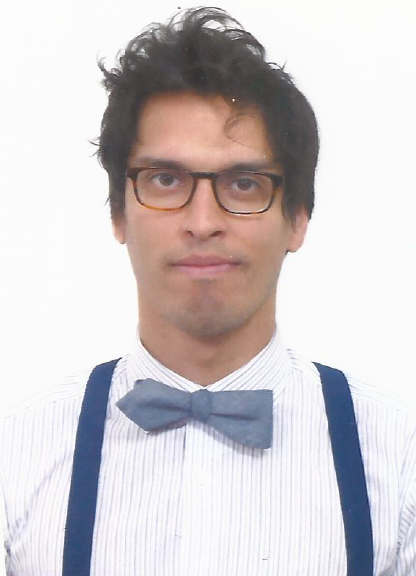
\includegraphics[width=0.2\textwidth]{1-introduction/img/georges-louis-joseph-labreche.jpg}  & \textbf{Georges L. J. Labrèche - Management Division}

\smallskip
\textit{Education}: BSc in Software Engineering with experience in technical leadership and project management in software development.

\smallskip
\textit{Responsibilities}: Acting as Systems Engineer / Project Manager and managing overall implementation of the project until the Critical Design Review (CDR). Establishing and overseeing product development cycle. Coordinating between different teams, project stakeholders, and documentation efforts.                          
\bigskip
\\

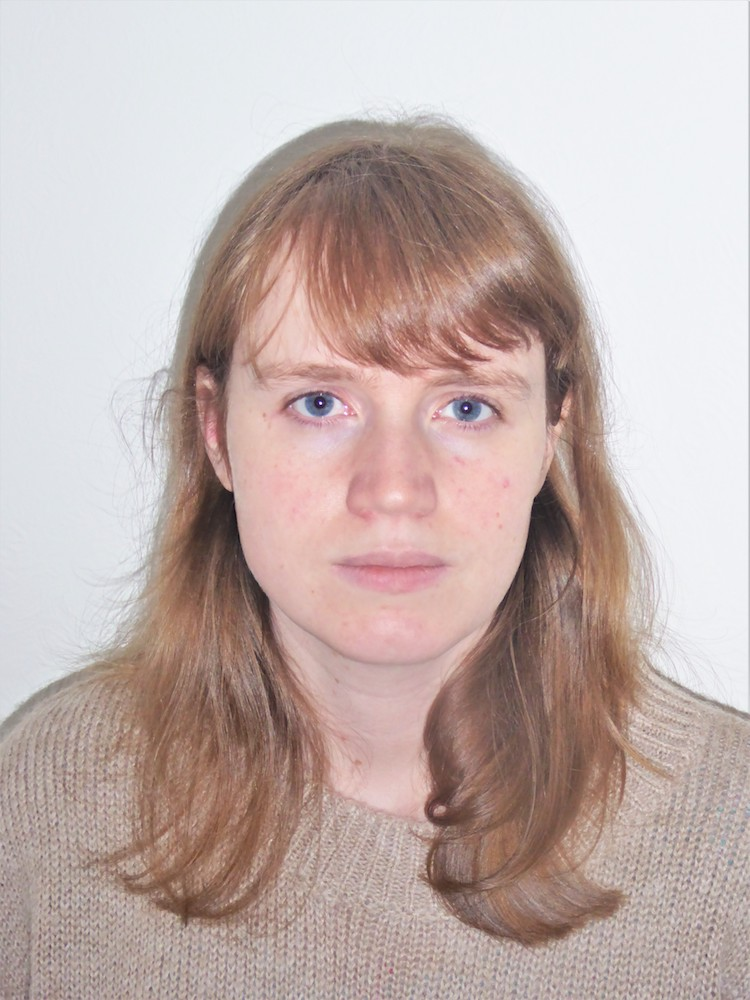
\includegraphics[width=0.2\textwidth]{1-introduction/img/natalie-lawton.jpg} & \textbf{Natalie Lawton - Management and Electrical Division}

\smallskip
\textit{Education}: MEng in Aerospace Engineering. Previous experience in UAV avionic systems and emissions measurement techniques.

\smallskip
\textit{Responsibilities}: Acting as Deputy Systems Engineer / Project Manager until the CDR. Assuming role of System Engineer / Project Manager after the CDR until end of project. Supporting designing and implementing cost-effective circuitry using analysis and computer-aided design; Reviewing and testing proposed designs; recommending modifications following prototype test results; assembling designed circuitry. 
\bigskip
\\

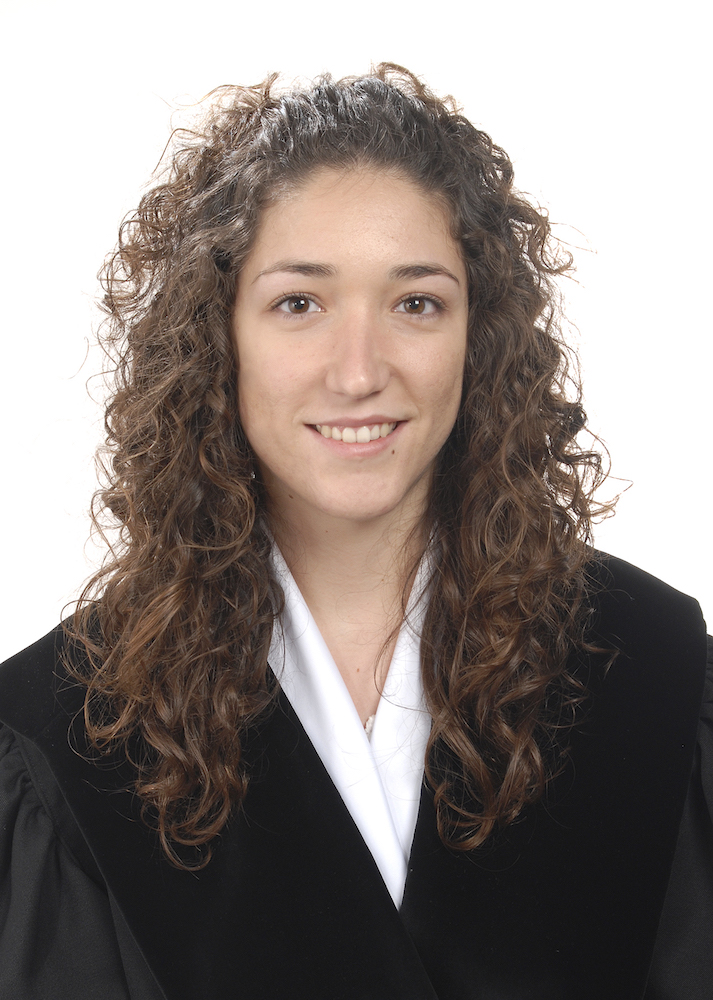
\includegraphics[width=0.2\textwidth]{1-introduction/img/agues-paszkowsky.jpg} & \textbf{Nuria Agües Paszkowsky - Scientific Division}

\smallskip
\textit{Education}: BSc in Aerospace Engineering.

\smallskip
\textit{Responsibilities}: Defining experiment parameters; data analysis; interpreting and documenting measurements; research on previous CAC experiments for comparative analysis purposes; contacting researchers or institutions working on similar projects; exploring potential partnership with researchers and institutions, evaluating the reliability of the proposed AAC sampling system; conducting measurements of collected samples; documenting and publishing findings. 
\bigskip
\\

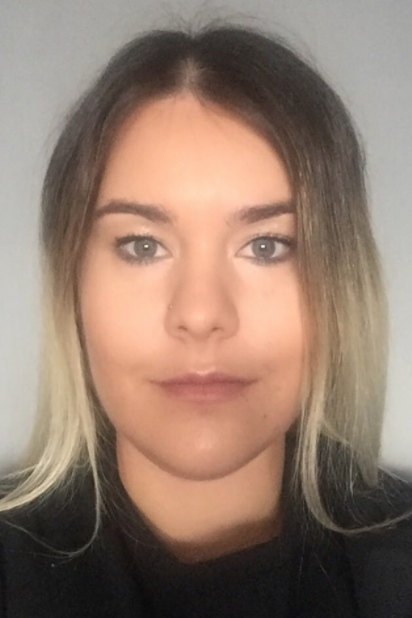
\includegraphics[width=0.2\textwidth]{1-introduction/img/kiki-blazaki.jpg} & \textbf{Kyriaki Blazaki - Scientific Division}

\smallskip
\textit{Education}: BSc in Physics.


\smallskip
\textit{Responsibilities}: Coordinating between the Scientific Division and the Project Manager; defining experiment parameters; data analysis; interpreting and documenting measurements; research on previous CAC experiments for comparative analysis purposes; evaluating the reliability of the proposed AAC sampling system; conducting measurements of collected samples; documenting and publishing findings. 
\bigskip
\\

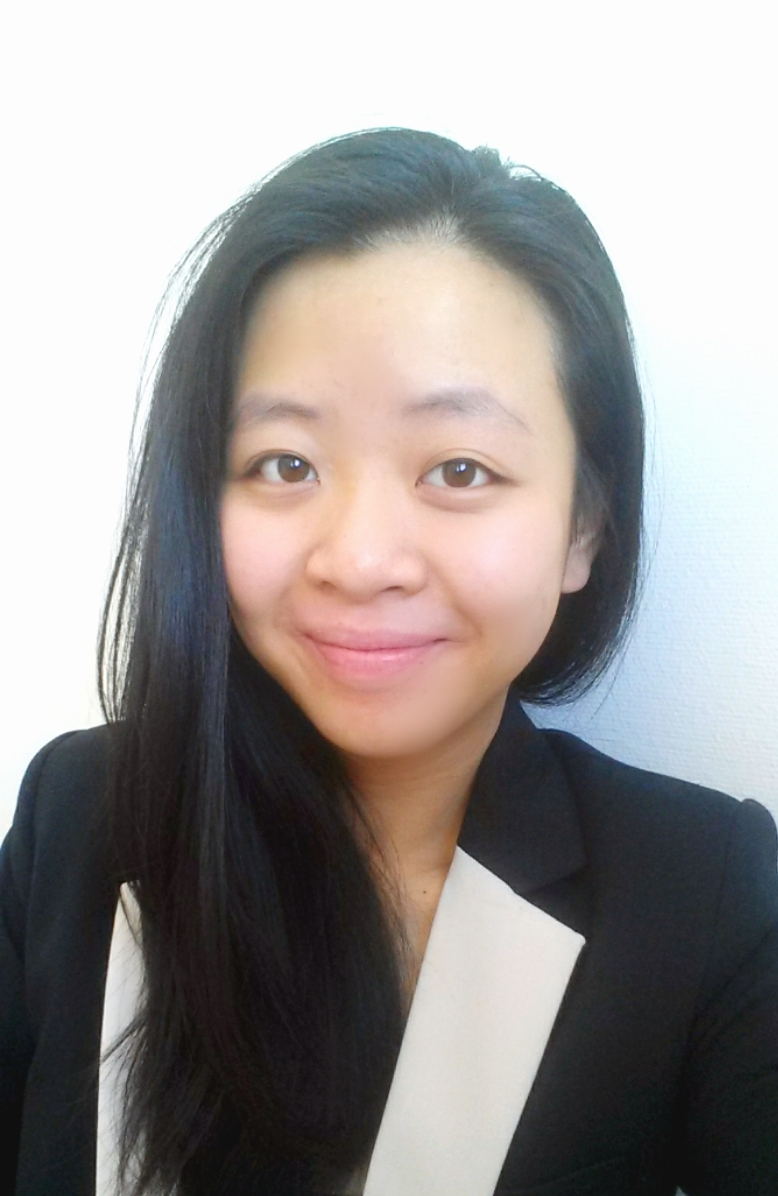
\includegraphics[width=0.2\textwidth]{1-introduction/img/emily-chen.jpeg} & \textbf{Emily Chen - Mechanical Division}

\smallskip
\textit{Education}: MSc in Space Engineering (4th Year).


\smallskip
\textit{Responsibilities}: Mechanical designing and assembly of CAC subsystem; analyzing the test results and changing the design as needed in collaboration with the team lead; integrating and assembling final design. 
\bigskip
\\

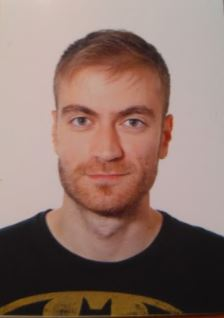
\includegraphics[width=0.2\textwidth]{1-introduction/img/jordi-coll-ortega.jpg} & \textbf{Jordi Coll Ortega - Mechanical Division}

\smallskip
\textit{Education}: BASc in Aerospace Vehicle Engineering.

\smallskip
\textit{Responsibilities}: Designing or redesigning cost-effective mechanical devices using analysis and computer-aided design; developing and testing prototypes of designed devices; analyzing the test results and changing the design as needed in collaboration with the team lead; integrating and assembling final design.
\bigskip
\\


\includegraphics[width=0.2\textwidth]{1-introduction/img/gustav-dryssen.jpg} & \textbf{Gustav Dyrssen - Software Division}

\smallskip
\textit{Education}: MSc in Space Engineering (4th Year).

\smallskip
\textit{Responsibilities}: Leading quality assurance and testing efforts; Enforcing software testing best practices such as continuous integration testing and regression testing; reviewing requirements and specifications in order to foresee potential issues; provide input of functional requirements; advising on design; formalizing test cases; tracking defects and ensuring their resolution; facilitating code review sessions; supporting software implementation efforts.     
\bigskip
\\



\includegraphics[width=0.2\textwidth]{1-introduction/img/erik-fagerstrom.jpg} & \textbf{Erik Fagerström - Thermal Division}

\smallskip
\textit{Education}: MSc in Space Engineering (4th Year).


\smallskip
\textit{Responsibilities}: Coordinating between the Thermal Division and the Project Manager. Planning project thermal analysis and testing strategy. Thermal simulations of proposed designs and analyze result.
\bigskip
\\


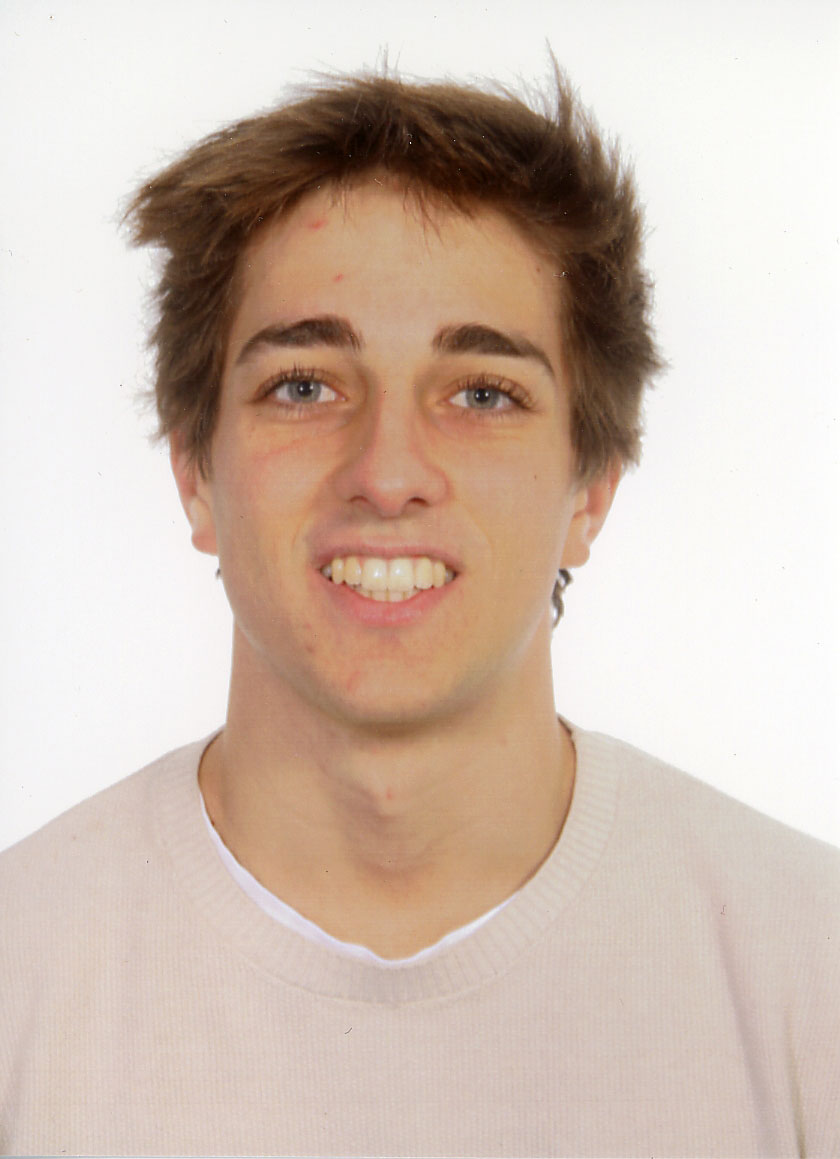
\includegraphics[width=0.2\textwidth]{1-introduction/img/pau-molas-roca.jpg} & \textbf{Pau Molas Roca - Mechanical Division}

\smallskip
\textit{Education}: BSc in Aerospace Technology Engineering, Mechanical experience.

\smallskip
\textit{Responsibilities}: Coordinating between the Mechanical Division and the Project Manager; designing or redesigning cost-effective mechanical devices using analysis and computer-aided design; producing details of specifications and outline designs; overseeing the manufacturing process for the devices; identifying material and component suppliers; integrating and assembling final design.   \bigskip
\\



\includegraphics[width=0.2\textwidth]{1-introduction/img/emil-nordqvist.jpg} & \textbf{Emil Nordqvist - Electrical Division}

\smallskip
\textit{Education}: MSc in Space Engineering (4th Year).

\smallskip
\textit{Responsibilities}: Quality assurance of circuit design and implementation. Developing, testing, and evaluating theoretical designs.  \bigskip
\\

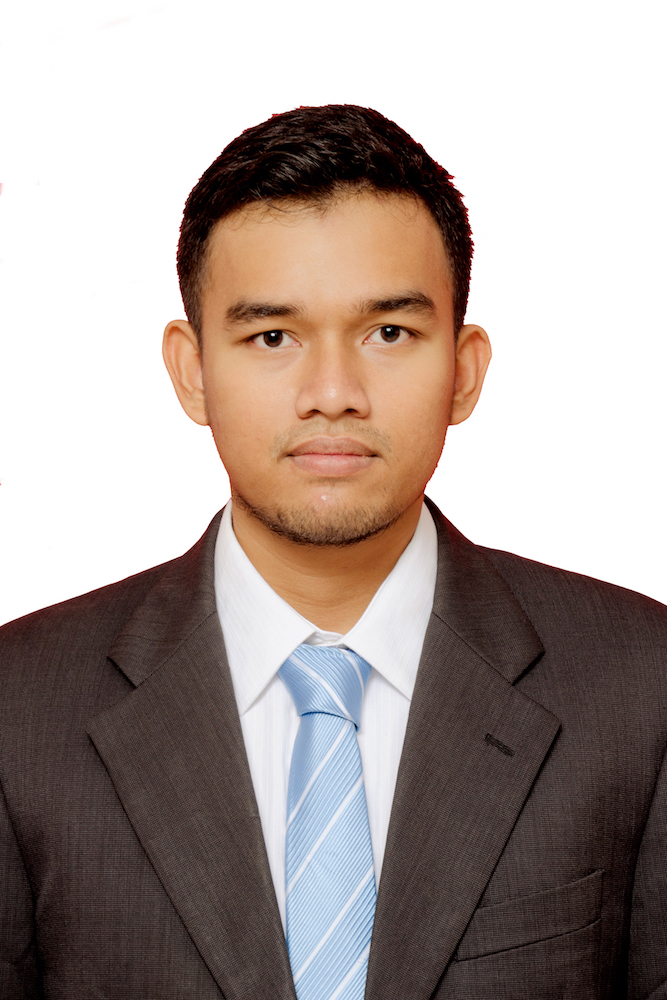
\includegraphics[width=0.2\textwidth]{1-introduction/img/muhammad-ansyar-rafi-putra.jpg} & \textbf{Muhammad Ansyar Rafi Putra - Software Division}

\smallskip
\textit{Education}: BSc in Aerospace Engineering.


\smallskip 
\textit{Responsibilities}: Coordinating between the Software Division and the Project Manager; gathering software requirements; formalizing software specifications; drafting architecture design, detailed design; leading software implementation efforts.
\bigskip
\\

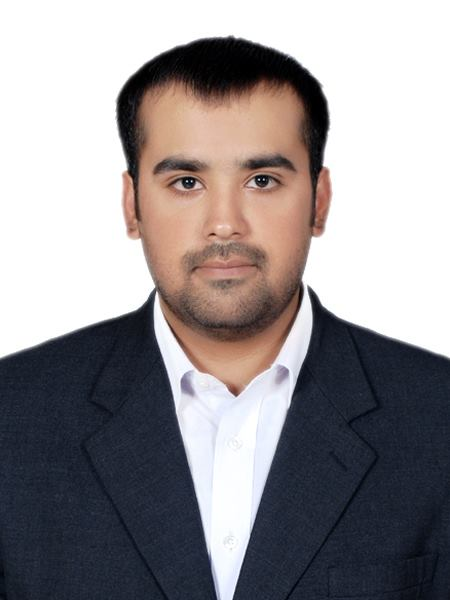
\includegraphics[width=0.2\textwidth]{1-introduction/img/hamad-saddiqi.jpg} & \textbf{Hamad Siddiqi - Electrical Division}

\smallskip
\textit{Education}: BSc in Electrical Engineering with experience in telecommunication industry and electronics.

\smallskip
\textit{Responsibilities}: Coordinating between the Electrical Division and the Project Manager; designing and implementing cost-effective circuitry using analysis and computer-aided design; producing details of specifications and outline designs; developing, testing, and evaluating theoretical designs; identifying material as well as component suppliers. 
\bigskip
\\


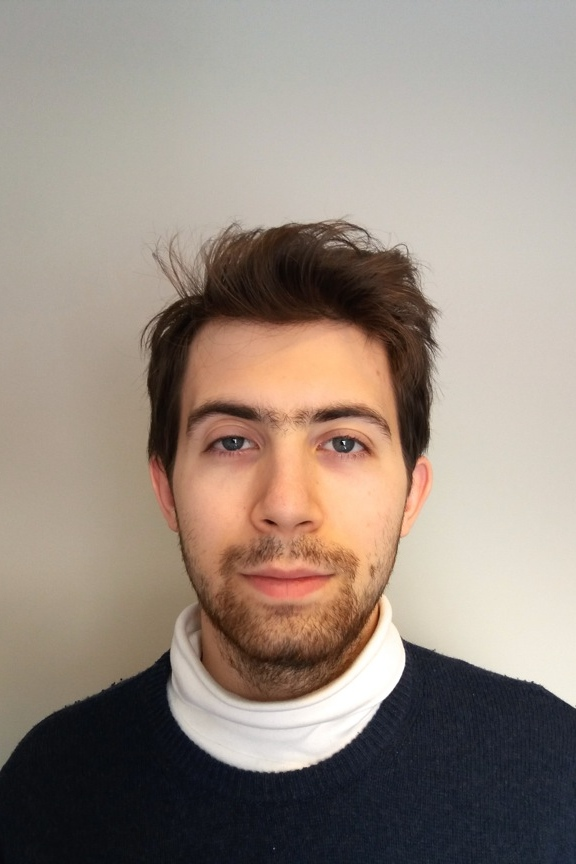
\includegraphics[width=0.2\textwidth]{1-introduction/img/ivan-zankov.jpg} & \textbf{Ivan Zankov - Thermal Division}

\smallskip
\textit{Education}: BEng in Mechanical Engineering.

\smallskip
\textit{Responsibilities}: Thermal analysis of proposed designs and analysis result based recommendations.                                                         

\\
\label{tab:people}
\end{longtable}
\raggedbottom

\pagebreak
\section{Experiment Requirements and Constraints}
\subsection{Functional Requirements}

\begin{enumerate}
    \item[F.2] The experiment \textit{shall} collect air samples by the CAC.
    \item[F.3] The experiment \textit{shall} collect air samples by the AAC.
    \item[F.9] The experiment \textit{should} measure the air intake flow to the AAC.
    \item[F.10] The experiment \textit{shall} measure the air pressure.
    \item[F.11] The experiment \textit{shall} measure the temperature.
    \item[F.12] The experiment \textit{shall} collect data on the humidity.
\end{enumerate}
\pagebreak
\subsection{Performance Requirements}

\begin{enumerate}
    %\item The programmable sampling rate of the pressure sensor \textit{shall} not be lesser than .
    \item[P.12] The accuracy of the ambient pressure measurements \textit{shall} be -1.5/+1.5 mbar for 25$\degree$C.
    \item[P.13] The accuracy of temperature measurements \textit{shall} be +3.5/-3$\degree$C (max) for condition of -55$\degree$C to 150$\degree$C.
    \item[P.23] The temperature sensor sampling rate \textit{shall} be 1 Hz.\label{newsamplerate}
    \item[P.24] The temperature of the Pump \textit{shall} be between 5$\degree$C and 40$\degree$C. 
    \item[P.25] The minimum volume of air in the bags for analysis \textit{shall} be 0.18 L at ground level.
    \item[P.26] The flow rate of the pump \textit{shall} be between 8 to 3 L/min from ground level up to 24 km altitude.
    \item[P.27] The accuracy range of the sampling time, or the resolution, \textit{shall} be less than 52.94 s, or 423.53 m.
    \item[P.28] The pressure sensor sampling rate \textit{shall} be 1 Hz.\label{newsamplerate}
    \item[P.29] The airflow sensor sampling rate \textit{shall} be 1 Hz.\label{newsamplerate}
    \item[P.30] The accuracy of the pressure measurements inside the tubing and sampling bags \textit{shall} be -0.005/+0.005 bar for 25$\degree$C.
    
 \end{enumerate} 
\pagebreak
\subsection{Design Requirements}

\begin{enumerate}[label=D.\arabic*]
    \item The experiment \textit{shall} operate in the temperature profile of the BEXUS flight.
    \item The experiment \textit{shall} operate in the vibration profile of the BEXUS flight.
    \item \st{The experiment \textit{shall} not disturb or harm the launch vehicle.}\textsuperscript{\ref{fn:unnecessary-requirement}}
    \item The experiment's communication system \textit{shall} be compatible with the gondola's E-link system.
    \item The experiment's power supply \textit{shall} be compatible with the gondola's provided power.
    \item \st{The experiment \textit{shall} not disturb other experiments on the gondola.}\textsuperscript{\ref{fn:unnecessary-requirement}}
    \item The total DC current draw \textit{should} be below 1.8 A.
    \item The total power consumption \textit{should} be below 374 Wh.
    \item \st{The experiment \textit{shall} be able to operate in low pressure conditions (10-15 mbar) up to 30 km altitude.}\footnote{Repeated in D18\label{fn:repeat-d18}}
    \item \st{The components of the experiment \textit{shall} operate within their temperature ranges.}\textsuperscript{\ref{fn:unnecessary-requirement}}
    \item \st{The OBC \textit{shall} be able to autonomously control the heaters.}\textsuperscript{\ref{fn:unnecessary-requirement}}
    \item \st{The ground station GC \textit{shall} be able to display some of the received data.}\textsuperscript{\ref{fn:unnecessary-requirement}}
    \item \st{The experiment \textit{shall} be able to survive and operate between -30\degree C and 60\degree C.}\textsuperscript{\ref{fn:unnecessary-requirement}}
    \item \st{The external components that are directly exposed to the outside environment \textit{shall} be able to operate at -70\degree C.}\textsuperscript{\ref{fn:unnecessary-requirement}}
    \item \st{The watchdog \textit{should} be able to reset the system.}\textsuperscript{\ref{fn:unnecessary-requirement}}
    \item The experiment \textit{shall} be able to autonomously turn itself off just before landing.
    \item The experiment box \textit{shall} be placed with at least one face exposed to the outside.
    \item The experiment \textit{shall} operate in the pressure profile of the BEXUS flight.
    \item The experiment \textit{shall} operate in the vertical and horizontal accelerations profile of the BEXUS flight.
    \item \st{The experiment \textit{shall} operate in the
    horizontal accelerations profile of the BEXUS flight.}\footnote{Combined with D19\label{fn:combi-d19}}
    \item The experiment \textit{shall} be attached to the gondola's rails.
    \item The telecommand data rate \textit{shall} not be over 10 kb/s.
    \item The air intake rate of the air pump \textit{shall} be minimum 3 L/min at 24 km altitude.
    \item The temperature of the Brain \textit{shall} be between -10$\degree$C and 25$\degree$C.
    \item \st{The temperature of the Brain level 2 \textit{shall} be between 0$\degree$C and 25$\degree$C.} \footnote{Combined with D24\label{fn:combi-d24}}
    \item The air sampling systems \textit{shall} filter out all water molecules before filling the sampling bags.
    \item The total weight of the experiment \textit{shall} be less than 28 kg.
    \item The AAC box \textit{shall} be able to fit at least $6$ air sampling bags.
    \item The CAC box \textit{shall} take less than 3 minutes to be removed from the gondola without removing the whole experiment.
    \item The AAC \textit{shall} be re-usable for future balloon flights.
\end{enumerate}
\pagebreak
\pagebreak
\subsection{Operational Requirements}

\begin{enumerate}
    \item[O.13] The experiment \textit{should} function automatically.
    \item[O.14] The experiment's air sampling mechanisms \textit{shall} have a manual override.
\end{enumerate} 
\pagebreak
\subsection{Constraints}

\begin{enumerate}[label=C.\arabic*]
    \item Constraints specified in the BEXUS User Manual.
    \item \st{The person-hours allocated to project implementation is limited by university related factors such as exams, assignments, and lectures.}\textsuperscript{\ref{fn:unnecessary-requirement}}
    \item \st{Budget limited to TBD.}\textsuperscript{\ref{fn:unnecessary-requirement}}
    \item \st{The dimensions show a minimum print area of 50 x 50 cm and 65 cm height experiment box.}\textsuperscript{\ref{fn:unnecessary-requirement}}
\end{enumerate}



\pagebreak
\section{Project Planning}

\subsection{Work Breakdown Structure}

The team is categorized into different groups of responsibilities with dedicated leaders who will report to and coordinate with the Project Manager. Leadership may be organized on a rotational basis should the need arise. The formation of these divisions constitute a work breakdown structure in which is illustrated in Figure \ref{fig:work-breakdown-structure}.


The interaction between the divisions will be refined over the course of project implementation to acknowledge the interdisciplinary nature of the experiment around a Payload / Platform scheme.

The Management is composed of a Project Manager and a Deputy Project Manager, both acting as Systems Engineer and managing overall implementation of the project. The Project Manager is responsible for establishing and overseeing product development cycle; coordinating between different teams, project stakeholders, and documentation efforts; outreach and public relations; Fundraising; monitoring and reporting; system integration; and quality assurance. The Deputy Project Manager assists the Project Manager in all management duties in a manner that ensures replaceability when necessary.

The Scientific Division is responsible for defining experiment parameters; data analysis; interpreting and documenting measurements; researching previous CAC experiments for comparative analysis purposes; evaluating the reliability of the proposed AAC sampling system; conducting measurements of collected samples; documenting and publishing findings; defining experiment parameters; contacting researchers or institutions working on similar projects; exploring potential partnership with researchers and institutions; documenting and publishing findings.

The Mechanical Division is responsible for designing or redesigning cost-effective mechanical devices using analysis and computer-aided design; producing details of specifications and outline designs; overseeing the manufacturing process for the devices; identifying material and component suppliers; developing and testing prototypes of designed devices; analyzing test results and changing the design as needed; and integrating and assembling final design.

The Electrical Division is responsible for designing and implementing cost-effective circuitry using analysis and computer-aided design; producing details of specifications and outline designs; developing, testing, and evaluating theoretical designs; identifying material as well as component suppliers; reviewing and testing proposed designs; recommending modifications following prototype test results; and assembling designed circuitry.

The Software Division is responsible for gathering software requirements; formalizing software specifications; drafting architecture design; leading software implementation efforts; leading quality assurance and testing efforts; enforcing software testing best practices such as continuous integration testing and regression testing; reviewing requirements and specifications in order to foresee potential issues; providing input for functional requirements; advising on design; formalizing test cases; tracking defects and ensuring their resolution; facilitating code review sessions; and supporting software implementation efforts.

The Thermal Division is responsible for ensuring thermal regulation of the payload as per operational requirements of all experiment components; evaluating designs against thermal simulation and propose improvements; managing against mechanical design and electrical power limitations towards providing passive and active thermal control systems.

\begin{landscape}
\begin{figure}[p]
    \begin{align*}
        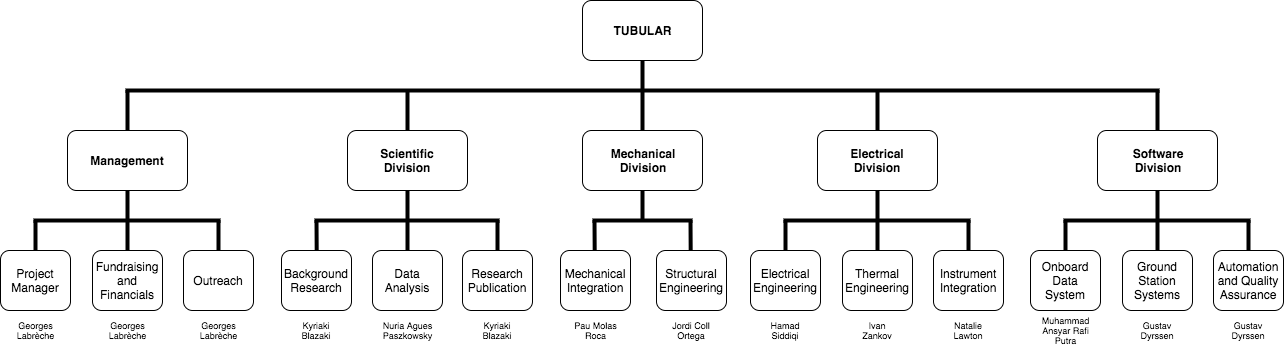
\includegraphics[width=24cm]{3-project-planning/img/work-breakdown-structure.png}
    \end{align*}
    \caption{Work Breakdown Structure}\label{fig:work-breakdown-structure}
\end{figure}
\end{landscape}
\pagebreak
\subsection{Schedule}

Scheduling of the project is presented in a Gantt Chart overview on Figure \ref{fig:schedule-gantt-chart}. Exam period constraints were included in order to evaluate risks in person-day allocations to project implementation. It was expected during exam periods the team work output would be lower than usual but project activities did continue, with time planned accordingly to accommodate this:

\begin{figure}[H]
    \begin{align*}
        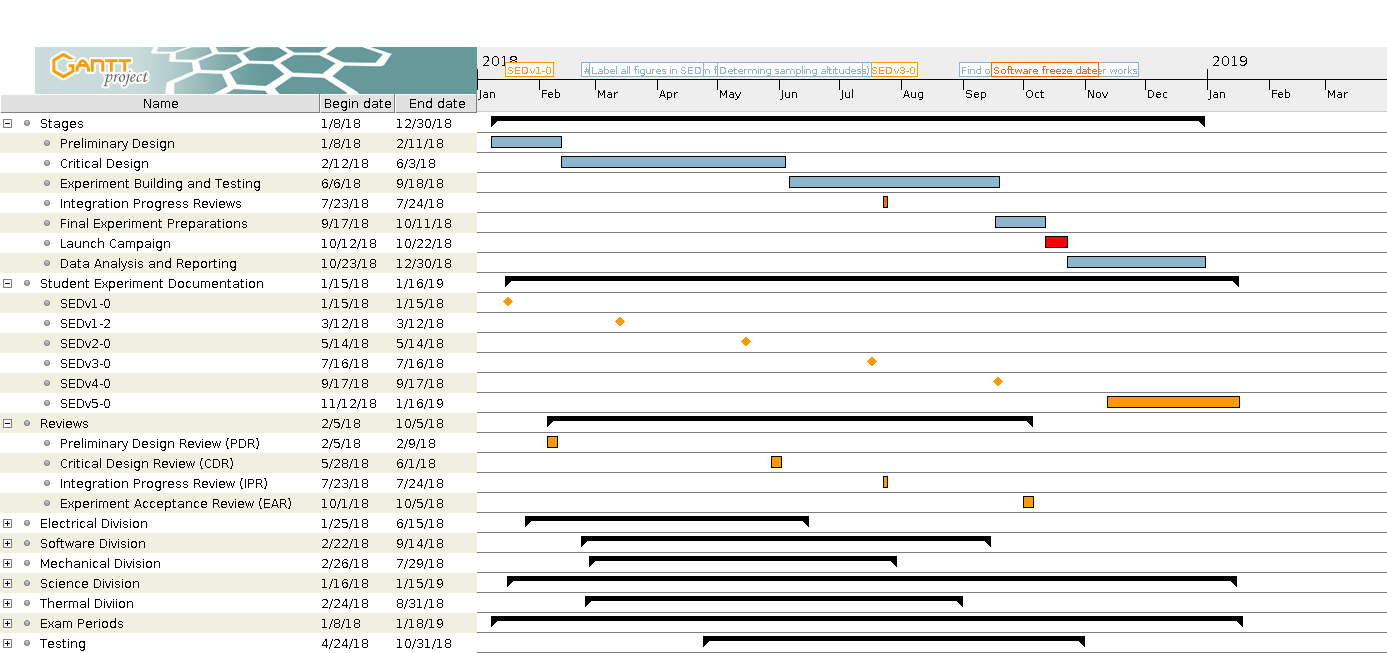
\includegraphics[width=1\linewidth]{3-project-planning/img/BEXUS-SED-GanttChart-Overview.png}
    \end{align*}
    \caption{Project Schedule Gantt Chart.}\label{fig:schedule-gantt-chart}
\end{figure}

An expanded version of the Gantt Chart with detailed listing of all sub-tasks not shown in Figure \ref{fig:schedule-gantt-chart} can be found in Appendix \ref{sec:appF}. This expanded Gantt Chart includes all tasks related to the test plan and internal deadlines were set so that a first draft of the documentation was completed one week in advance to allow contents to be checked. Build and test internal deadlines were also placed one week in advance to allow a buffer in case things did not go as expected. The tests were scheduled for as early as possible to allow time for rescheduling if the result was a fail. With some high priority tests, see Section \ref{sec:5.2.1-testpriority}, it was expected these would be very difficult to reschedule therefore extra time was built into the test duration to allow for multiple attempts at the test.


\pagebreak
\subsection{Resources}

\subsubsection{Manpower}
The TUBULAR team is categorized into divisions as summarized in Table \ref{tab:divisions-members}:

\begin{table}[H]
\centering
\resizebox{\textwidth}{!}{%
\begin{tabular}{|l|l|l|l|l|}
\hline
\textbf{Management} & \textbf{Scientific}    & \textbf{Mechanical} & \textbf{Electrical} & \textbf{Software}          \\ \hline
Georges Labrèche*    & Kyriaki Blazaki*        & Pau Molas Roca*      & Hamad Siddiqi*       & Muhammad Ansyar Rafi Putra* \\ \hline
                    & Nuria Agues Paszkowsky & Jordi Coll Ortega   & Natalie Lawton      & Gustav Dyrssen             \\ \hline
                    &                        &                     & Ivan Zankov         &                            \\ \hline
\end{tabular}%
}
\caption{Project Divisions and Members (Asterisks Denote Division Leaders)}
\label{tab:divisions-members}
\end{table}
\raggedbottom

The experience of TUBULAR team members are listed in Table \ref{tab:team-member-experience}:

% Please add the following required packages to your document preamble:
% \usepackage{graphicx}
\begin{table}[H]
\centering
\begin{tabular}{|l|m{11cm}|}
\hline
\textbf{Team Member} & \textbf{Project Related Experience} \\ \hline
Georges L. J. Labrèche & BSc in Software Engineering with experience in technical leadership and project management in software development.\\ \hline
Nuria Agues Paszkowsky & BSc in Aerospace Engineering.\\ \hline
Kyriaki Blazaki & BSc in Physics. \\ \hline
Emily Chen & MSc in Space Engineering (4th Year). \\ \hline
Jordi Coll Ortega &  BSc in Aerospace Vehicle Engineering. \\ \hline
Gustav Dyrssen &  MSc in Space Engineering (4th Year).\\ \hline
Erik Fagerström & MSc in Space Engineering (4th Year). \\ \hline
Natalie Lawton & MEng in Aerospace Engineering. Previous experience in UAV avionic systems and emissions measurement techniques. \\ \hline
Muhammad Ansyar Rafi Putra & BSc in Aerospace Engineering. \\ \hline
Pau Molas Roca & BSc in Aerospace Technology Engineering, Mechanical experience. \\ \hline
Emil Nordqvist & MSc in Space Engineering (4th Year). \\ \hline
Hamad Siddiqi & BSc in Electrical Engineering with experience in telecommunication industry and electronics.  \\ \hline
Ivan Zankov & BEng in Mechanical Engineering.\\ \hline
\end{tabular}
\caption{Project Related Experience of Team Members}
\label{tab:team-member-experience}
\end{table}
\raggedbottom

The initial projected effort to be contributed by each team member is of an average of 1.5 hour per person per day corresponding to a team total of 15 hours per day. Taking into account all team members, the efforts projected to be allocated to each stages of the project is summarized in Table \ref{tab:effort-allocation-stages}:

\begin{table}[H]
\centering
\begin{tabular}{lcc|c|c|c|c|}
\hline
\multicolumn{1}{|c|}{\multirow{2}{*}{\textbf{Stage}}} & \multicolumn{1}{c|}{\multirow{2}{*}{\textbf{\begin{tabular}[c]{@{}c@{}}Start\\ Date\end{tabular}}}} & \multirow{2}{*}{\textbf{\begin{tabular}[c]{@{}c@{}}End\\ Date\end{tabular}}} & \multirow{2}{*}{\textbf{\begin{tabular}[c]{@{}c@{}}Duration\\ (days)\end{tabular}}} & \multicolumn{3}{c|}{\textbf{Effort (hours)}} \\ \cline{5-7} 
\multicolumn{1}{|c|}{} & \multicolumn{1}{c|}{} &  &  & \textbf{Capacity} & \textbf{Actual} & \multicolumn{1}{l|}{\textbf{Diff. (\%)}} \\ \hline
\multicolumn{1}{|l|}{Preliminary Design} & \multicolumn{1}{c|}{08/01} & 11/02 & 35 & 525 & 708 & +29.68 \\ \hline
\multicolumn{1}{|l|}{Critical Design} & \multicolumn{1}{c|}{12/02} & 03/06 & 112 & 1,680 & 2,649 & +57.66 \\ \hline
\multicolumn{1}{|l|}{Experiment Building and Testing} & \multicolumn{1}{c|}{04/06} & 16/09 & 105 & 2,048 & 1,943 & -5.40 \\ \hline
\multicolumn{1}{|l|}{Final Experiment Preparations} & \multicolumn{1}{c|}{17/09} & 11/10 & 25 & 488 & 571 & +17.00 \\ \hline
\multicolumn{1}{|l|}{Launch Campaign} & \multicolumn{1}{c|}{12/10} & 22/10 & 10 & 390 & 777 & +99.23 \\ \hline
\multicolumn{1}{|l|}{Data Analysis and Reporting} & \multicolumn{1}{c|}{23/10} & 30/01 & 69 & 1,346 & 245 & -81.78 \\ \hline
\multicolumn{1}{r}{\textbf{}} & \multicolumn{1}{l}{} & \multicolumn{1}{r|}{\textbf{Total:}} & \textbf{356} & \textbf{7,989} & \textit{6939} & \textit{-13.14} \\ \cline{4-7} 
\end{tabular}
\caption{Project Effort Allocation per Project Stages.}
\label{tab:effort-allocation-stages}
\end{table}

All TUBULAR team members are based in Kiruna, Sweden, just 40 kilometers from Esrange Space Center. Furthermore, all team members are enrolled in LTU Master programmes in Kiruna and thus expected to remain in Kiruna during the entire project period. Special attention will have to be made for planning during the summer period where many team members are expected to travel abroad. An initial timeline of team member availability  until January 2019 is available in Appendix \ref{sec:appD}. A significant risk can be observed during the summer months from June to August where most members will only be partially and some completely unavailable. Team member availability and work commitments over the summer still need to be negotiated and finalized across team members in order to reduce incurred risks to the project. Furthermore, the Project Manager role will have to be assigned to another team member due to extended unavailability and partial availability.

As part of their respective Master programmes, all TUBULAR team members are enrolled in a project course at LTU. The TUBULAR project acts as the course's project for all team members from which they will obtain ECTS credits. This course is supervised by Dr. Thomas Kuhn, Associate Professor at LTU.

\pagebreak
\subsubsection{Budget}
LTU will provide financial assistance for part of the hardware expenses, approximately 250 EUR per team member. This brings the total budget to 2 500 EUR thus far. However, the total cost of the project is 8 295.04 EUR\footnote{The cost of some items have been estimated due to lack of direct quotes from vendors. A total error margin of 5\% has been included in the final budget to account for possible estimation errors.}. In order to fill this budget gap, the following potential sources of funding are to be explored throughout the first stages of the project implementation:

\begin{itemize}
    \item The Swedish National Space Board, SNSB, will be reached out to during their next open call to researchers in Sweden to apply for funding for Space Research, including Earth Observation Research.
    \item The Swedish Research Council typically opens calls for \enquote{Proof of Concept Grant – Life science} as well as \enquote{Natural and Engineering Sciences} research grants to which an application will be sent to during the upcoming 2018 calls.
    \item Meteorological institutes, research initiatives, researchers, academic institutions, and institutional donors involved in climate change will be reached out to for contributions based on the interest of collaborating in the experiment.
    \item Third-party providers of required equipment, components, and materials will be approached with an opportunity for these providers to sponsor the project through donation before considering the related expenses. Visibility of the experiment through the planned outreach programs will serve as a visibility incentive to encourage such contributions.
    \item A small online crowdfunding campaign will be organized that will primarily target contributions from the team members' first and second degree contacts.
\end{itemize}

The project budget is detailed in Table \ref{tab:budget-table}. The budget table does not include costs related to component redundancy and as such consist of the minimum cost to build the experiment. Not included in the total are components supplied by partners and potential sponsors (e.g. the CAC tube supplied by FMI). Funding from LTU covers 30\% of the total costs while it is projected that a SNSB grant will cover 34\%. The remaining costs are associated with the air sampling bags for which sponsorship will actively be sought from a manufacturer.

\pagebreak
%\begin{longtable}[]
{|c|l|l|}
\hline
\multicolumn{2}{|l|}{\textbf{Expenses and Revenue per Department}} & Amount (\EUR{}) \\ \hline
\multicolumn{1}{|c|}{\multirow{5}{*}{\textbf{Electronics}}} & Components\footnote{Total cost for components is based upon Table \ref{tab:electrical-components}.} (excluding valves) & 450 \\
\multicolumn{1}{|c|}{} & Valves & 2000 \\
\multicolumn{1}{|c|}{} & Shipping Costs & 100 \\
\multicolumn{1}{|c|}{} & Tools and Equipment & 200 \\ \cline{2-3} 
\multicolumn{1}{|c|}{} & \textbf{Total Electronics Cost} & 2750 \\ \hline
\multicolumn{1}{|c|}{\multirow{6}{*}{\textbf{Mechanics}}} & Components\footnote{Total cost for mechanics is based upon Table \ref{tab:mechanical-components}.} & 450 \\
\multicolumn{1}{|c|}{} & Manufacturing & TBD \\
\multicolumn{1}{|c|}{} & Testing (Structural and Thermal) & TBD \\
%\multicolumn{1}{|c|}{} & Shipping Costs & TBD \\
\cline{2-3} 
\multicolumn{1}{|c|}{} & \textbf{Total Mechanics Cost} & TBD \\ \hline
\multicolumn{1}{|c|}{} & Project Visibility (badges, merch, website, publications, etc) & 250\\
\cline{2-3} 
\multicolumn{1}{|c|}{} & \textbf{Total Outreach} & TBD \\ \hline
\multicolumn{1}{l|}{} & \textbf{Total Costs} & TBD \\ \cline{2-3} 
\caption{Preliminary Budget Table}
\label{tab:budget-table}
\end{longtable}
\raggedbottom

\begin{table}[H]
    \begin{align*}
        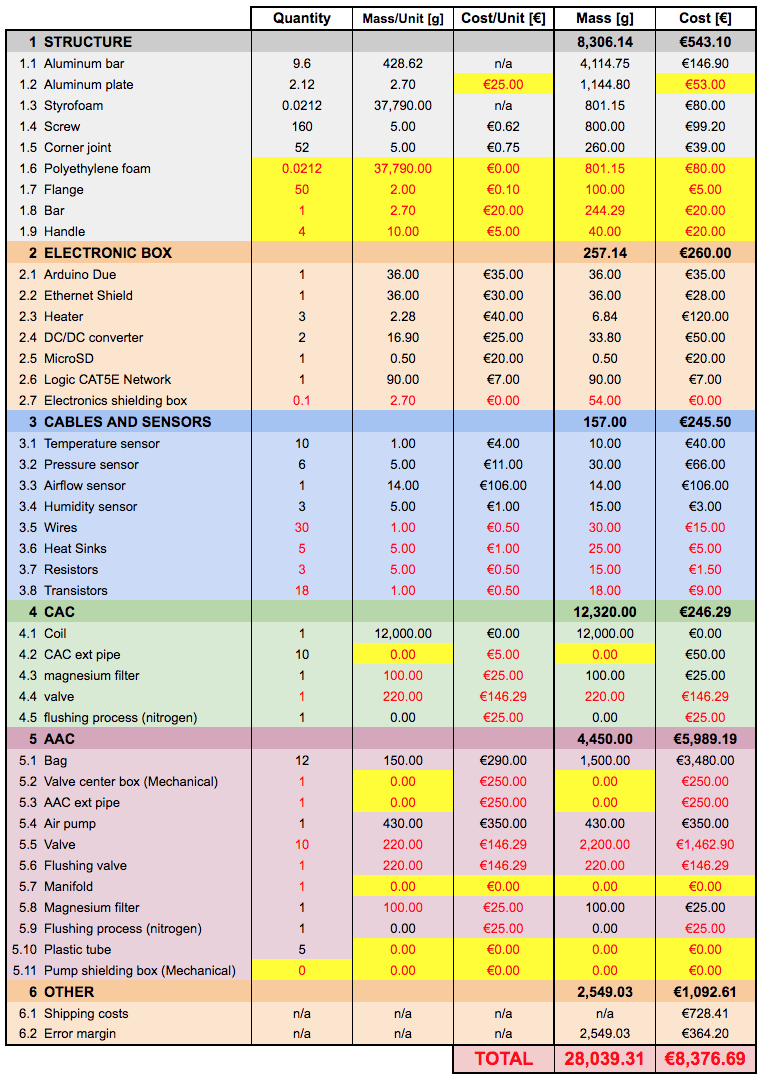
\includegraphics{3-project-planning/tables/budget-table.png}
    \end{align*}
    \caption{Project budget table. Values highlighted in yellow have yet to be determined/estimated. Number values in red have been estimated rather than determined by vendor quotes.}\label{tab:budget-table}
\end{table}


\subsubsection{External Support}

Partnership with the Finnish Meteorological Institute (FMI), and the Swedish Institute of Space Physics (IRF) will provide the team with technical guidance in implementing the sampling system. FMI’s experience in implementing past AirCore sample systems provide invaluable lessons learned towards conceptualizing, designing, and implementing the proposed AAC sampling system.

FMI is a key partner in the TUBULAR project, its scientific experts will advise and support the TUBULAR project by sharing knowledge, experience, and granting accessibility of equipment. FMI will provide the TUBULAR team with the AirCore stainless tube component of CAC subsystem as well as the post-flight gas analyzer. This arrangement requires careful considerations on the placement of the experiment in order to minimize hardware damage risks. These contributions will result in significant cost savings regarding equipment and component procurement.

Daily access to LTU's Space Campus in Kiruna will expose the team to scientific mentorship and expert guidance from both professors and researchers involved in the study of greenhouse gases and climate change. Dr Uwe Raffalski, Swedish institute of Space physics (IRF), Associate professor (Docent) is one of many researchers involved in climate study who is mentoring the team.
\pagebreak

\subsection{Outreach Approach}

The experiment as well as the REXUS/BEXUS programme and its partners will be promoted through the following activities:

\begin{itemize}
\item Research paper published in partnership with FMI detailing the sampling methodology, measurement result, analysis, and findings.
\item Collected data will be licensed as open data to be freely available to everyone to use and republish as they wish, without restrictions from copyright, patents or other mechanisms of control.
\item A website to summarize the experiment and provide regular updates. Backend web analytics included to gauge interest on the project through number of visitors and their origins (See Appendix \ref{sec:appE}).
\item Dedicated Facebook page used as publicly accessible logbook detailing challenges, progress, and status of the project. Open for comments and questions (See Figure \ref{fig:outreach-facebook} in Appendix \ref{sec:appE}).
\item Two Instagram accounts for short and frequent image and video focused updates. A primary Instagram account will be dedicated to project updates. A secondary account will reach out to a broader audience by focusing on space instruments in general and cross-reference TUBULAR related activities when relevant (See Figures \ref{fig:outreach-instagram}, \ref{fig:outreach-instagram-si-1}, and \ref{fig:outreach-instagram-si-2} in Appendix \ref{sec:appE}).
\item GitHub account to host all project software code under free and open source license (See Figure \ref{fig:outreach-github} in Appendix \ref{sec:appE}). Other REXUS/BEXUS teams will be invited to host their code in this account in what will hopefully become a centralized GitHub account and code archive for present and future REXUS/BEXUS projects.
\item Reddit Ask Me Anything (AMA) thread to discuss the project with community of online enthusiasts.
\item\enquote{Show and Tell} trips to local high schools and universities. Team members will be responsible to organize such presentations through any of their travel opportunities abroad.
\item Articles and/or blogposts about the project in team members' alma mater websites.
\item In-booth presentation and poster display in the seminars or career events at different universities. 
\item A thoroughly documented and user-friendly manual on how to build replicate and launch CAC and AAC sampling systems will be produced and published.
\end{itemize}
\pagebreak
\subsection{Risk Register}
\textbf{Risk ID}
\begin{enumerate}[label={}]
    \item TC – Technical/Implementation 
    \item MS – Mission (operational performance) 
    \item SF – Safety 
    \item VE – Vehicle 
    \item PE – Personnel 
    \item EN – Environmental 
    \item OR - Outreach
    \item BG - Budget
\end{enumerate}

Adapt these to the experiment and add other categories. 
Consider risks to the experiment, to the vehicle and to personnel. 

\textbf{Probability (P)}
\begin{enumerate}[label=\Alph*]
    \item Minimum – Almost impossible to occur 
    \item Low – Small chance to occur 
    \item Medium – Reasonable chance to occur 
    \item High – Quite likely to occur 
    \item Maximum – Certain to occur, maybe more than once
\end{enumerate}

\textbf{Severity (S)}
\begin{enumerate}
    \item Negligible – Minimal or no impact 
    \item Significant – Leads to reduced experiment performance 
    \item Major – Leads to failure of subsystem or loss of flight data 
    \item Critical – Leads to experiment failure or creates minor health hazards 
    \item Catastrophic – Leads to termination of the BEXUS programme, damage to the vehicle or injury to personnel 
\end{enumerate}

The rankings for probability (P) and severity (S) are combined to assess the overall risk classification, ranging from very low to very high and being coloured green, yellow, orange or red according to the SED guidelines.

\begin{landscape}



\begin{longtable}{|m{0.09\textwidth}| m{0.51\textwidth} |m{0.03\textwidth} |m{0.03\textwidth}|m{0.11\textwidth}| m{0.65\textwidth}|}

\hline
\textbf{ID} & \textbf{Risk (\& consequence if)} & \textbf{P} & \textbf{S} & \textbf{P * S} & \textbf{Action} \\ \hline
TC10 & Software fails to store data & B & 3 & \cellcolor[HTML]{FCFF2F}Low & Acceptable Risk: Extensive testing will be done. Using telemetry, all data gathered from sensors will be sent to ground station. \\ \hline
TC20 & Failure of several sensors & B & 3 & \cellcolor[HTML]{FCFF2F}Low & Acceptable Risk: Thermal test (Test Number 5) to approve the functionality of the experiment. \\ \hline
TC30 & Critical component is destroyed in testing & B & 1 & \cellcolor[HTML]{34FF34}Very Low & Acceptable Risk: Spare components can be ordered but for expensive ones, they will be ordered and tested early in the project in case we need to order more. \\ \hline
TC40 & Electrical connections dislodges or short circuits because of vibration or shock & B & 4 & \cellcolor[HTML]{FCFF2F}Low & Acceptable Risk. D-sub connections will be screwed in place. It will be ensured that there are no loose connections and zip ties will be used to help keep wires in place. Careful soldering and extensive testing will be applied. \\ \hline
TC50 & Experiment electronics fail due to long exposure to cold or warm temperatures & B & 3 & \cellcolor[HTML]{FCFF2F}Low & Acceptable Risk: Thermomechanical and thermoelectrical solutions will be simulated and tested in detail to help prevent this from happening. \\ \hline
TC60 & Software and electrical fail to control heaters causing temperature to drop or rise below or above operational range & B & 2 & \cellcolor[HTML]{34FF34}Very Low & Acceptable Risk: Tests will be performed prior to the flight to detect and minimize the risk of occurrence.The system will be monitored during flight and handled manually if necessary. \\ \hline
TC70 & Software fails to enter safe mode (may result in loss of data) & B & 3 & \cellcolor[HTML]{FCFF2F}Low & Acceptable Risk: Extensive testing will be done. \\ \hline
TC80 & On-board memory will be full (flight time longer than expected) & A & 2 & \cellcolor[HTML]{34FF34}Very Low & Acceptable Risk: The experiment shall go through testing and analysis to guarantee the onboard memory size is sufficient.\\ \hline
TC90 & Connection loss with ground station & A & 2 & \cellcolor[HTML]{34FF34}Very Low & Acceptable Risk: Experiment will be designed to operate autonomously. \\ \hline
TC100 & Software fails to control valves autonomously & B & 4 & \cellcolor[HTML]{FCFF2F}Low & Acceptable Risk: Extensive testing will be done. Telecommand will also be used to manually control the valves. \\ \hline
TC110 & Software fails to change modes autonomously & B & 4 & \cellcolor[HTML]{FCFF2F}Low & Acceptable Risk: Extensive testing will be done. Telecommand will also be used to manually change experiment modes. \\ \hline
TC120 & Complete software failure & B & 4 & \cellcolor[HTML]{FCFF2F}Low & Acceptable Risk: A long duration testing (bench test) will be performed to catch the failures early. \\ \hline
TC130 & Failure of fast recovery system & B & 2 & \cellcolor[HTML]{34FF34}Very Low & Acceptable Risk: Clear and simple instructions will be given to the recovery team. A test will take place before launch to ensure someone unfamiliar with the experiment can remove the CAC box. Test number: 12. \\ \hline
TC140 & The gas analyzer isn't correctly calibrated and returns inaccurate results & B & 4 & \cellcolor[HTML]{FCFF2F}Low & Acceptable Risk: Calibrate the gas analyzer before use.\\ \hline 
TC150 & Partnership with FMI does not materialize, resulting in loss of access to CAC coiled tube. & B & 2 & \cellcolor[HTML]{34FF34}Very Low & Acceptable Risk: Signed agreement has been obtained. AAC sample analysis results can be validated against available historical data from past FMI CAC flights. \\ \hline 
MS10 & Down link connection is lost prematurely & B & 2 & \cellcolor[HTML]{34FF34}Very Low & Acceptable Risk: Data will also be saved on SD card. \\ \hline
MS20 & Condensation on experiment PCBs which could causes short circuits & A & 3 & \cellcolor[HTML]{34FF34}Very Low & Acceptable Risk: The Brain will be sealed to prevent condensation. \\ \hline
MS30 & Temperature sensitive components that are essential to full the mission objective might be below their operating temperature. & C & 3 & \cellcolor[HTML]{FCFF2F}Low & Acceptable Risk: Safe mode to prevent the components to operate out of its operating temperature range. \\ \hline
MS40 & Experiment lands in water causing electronics failure & B & 1 & \cellcolor[HTML]{34FF34}Very Low & Acceptable Risk: Check if SD card needs waterproof shell or is waterproof in itself. Also, all the necessary data will be downloaded during the flight. \\ \hline
MS50 & Interference from other experiments and/or balloon & A & 2 & \cellcolor[HTML]{34FF34}Very Low & Acceptable Risk: no action. \\ \hline
MS60 & Balloon power failure & C & 2 & \cellcolor[HTML]{FCFF2F}Low & Acceptable Risk: Valves default state is closed so if all power is lost valves will automatically close preserving all samples collected up until that point. \\ \hline
MS70 & Sampling bags disconnect & C & 3 & \cellcolor[HTML]{FCFF2F}Low & Acceptable Risk: The affected bags could not collect samples. The connection between the spout of the bags and the T-union shall be double checked before flight. \\ \hline
MS71 & Sampling bags puncture & B & 3 & \cellcolor[HTML]{FCFF2F}Low & Acceptable Risk: The affected bags could not collect samples. Inner styrofoam walls have been choosen and no sharp edges will be exposed to avoid puncture from external elements. \\ \hline
MS72 & Sampling bags' hold time is typically 48h & C & 2 & \cellcolor[HTML]{FCFF2F}Low & Acceptable risk: Validation studies can demonstrate longer stability.  \\ \hline
MS80 & Pump failure & B & 4 & \cellcolor[HTML]{FCFF2F}Low & Acceptable Risk: A pump was chosen based on a previous similar experiment. The pump has also been tested in a low pressure chamber down to 10hPa and has successfully turned on and filled a sampling bag. \\ \hline
MS90 & Intake pipe blocked by external element & C & 3 & \cellcolor[HTML]{FCFF2F}Low & Acceptable Risk: The bags would not be filled and thus the AAC system would fail. An air filter will be placed in both intake and outlet of the pipe to prevent this. \\ \hline
MS100 & Expansion/Contraction of insulation & B & 2 &\cellcolor[HTML]{34FF34}Very Low & Acceptable Risk: The insulation selected has flown successfully on similar flights in the past. Test shall be done to see how it reacts in a low pressure environment. \\ \hline
MS110 & Sampling bags are over-filled resulting in bursting and loss of collected samples. & B & 3 & \cellcolor[HTML]{FCFF2F}Low & Acceptable Risk: Test will be performed at target ambient pressure levels to identify how long the pump needs to fill the sampling bags. Pressure sensors on board will monitor the in-bag pressure during sampling and no bag will ever be over pressured, therefore bags bursting should not be a concern. \\ \hline
SF10 & Safety risk due to pressurized vessels during recovery. & A & 1 & \cellcolor[HTML]{34FF34} Very Low & Acceptable Risk: The volume of air in the AAC decreases during descent because the pressure inside is lower than outside. The CAC is sealed at nearly sea level pressure, therefore there is only a small pressure difference.  \\ \hline
SF20 & Safety risk due to the use of chemicals such as magnesium perchlorate. & A & 3 & \cellcolor[HTML]{34FF34} Very Low & Acceptable Risk: The magnesium perchlorate will be kept in a sealed container or filter at all times. Magnesium perchlorate filters have been used before without any sealing problems. \\ \hline
VE10 & SD-card is destroyed at impact & B & 2 & \cellcolor[HTML]{34FF34}Very Low & Acceptable Risk: All data will be transmitted to the ground. Most of the data is the gas stored in the AAC and CAC. \\ \hline
VE20 & Gondola Fixing Interface & B & 4 & \cellcolor[HTML]{FCFF2F}Low & Acceptable Risk: The experiment box could detach from the gondola’s rails and the two boxes could detach one from the other. The experiment will be secured to the gondola and to each other with multiple fixings. These will also be tested. \\ \hline
VE30 & Structure damage due to bad landing & B & 3 & \cellcolor[HTML]{FCFF2F}Low & Acceptable Risk: Landing directly on a hard element could break the structure or the protective walls. Consistent design implemented to prevent it. \\ \hline
VE40 & Hard landing damages the CAC equipment & C & 3 & \cellcolor[HTML]{FCFF2F}Low & Acceptable Risk:  Structural analysis has been done and choosing a wall consisting of an aluminum sheet and Styrofoam to dampen the landing. \\ \hline
VE50 & Hard landing damages the AAC equipment & C & 3 & \cellcolor[HTML]{FCFF2F}Low & Acceptable Risk:  Structural analysis has been done and choosing a wall consisting of an aluminum sheet and Styrofoam to dampen the landing. \\ \hline
EN10 & Vibrations from pump affect samples & C & 1 & \cellcolor[HTML]{34FF34}Very Low & Acceptable Risk: Vibrations do not affect the sampled air. No action required. \\ \hline
EN20 & The air samples must be protected from direct sunlight and stored above 0 \degree C to prevent condensation & C & 3 & \cellcolor[HTML]{FCFF2F}Low & Acceptable Risk: Stratospheric air is generally dry and water vapor concentrations are higher closer to the surface. In addition magnesium perchlorate dryers will be used to minimizing the risk of condensation.    \\ \hline 
PE10 & Change in Project Manager after the CDR introduces a gap of knowledge in management responsibilities. & E & 1 & \cellcolor[HTML]{FCFF2F}Low & Acceptable Risk: A Deputy Project Manager is selected at an early stage and is progressively handed over project management tasks and responsibilities until complete handover after the CDR. The previous Project Manager remotely assists the new Project Manager until the end of the project. The Deputy Project Manager is also part of the Electrical Division so a new team member has been included to that division in order compensate for the Deputy Project Manager's reduced bandwidth to work on Electrical Division tasks once she is appointed Project Manager.\\ \hline 
PE20 & Team members from the same division are unavailable during the same period over the summer. & C & 2 & \cellcolor[HTML]{FCFF2F}Low & Acceptable Risk: Summer travel schedules have been coordinated among team members so that there is at least one member from each division available during the summer. \\ \hline
PE30 & No one from management is available to oversee the work for a reasonable period. & B & 2 & \cellcolor[HTML]{34FF34}Very Low & Acceptable Risk: Management summer travel schedules have been planned to fit around known deadlines. There will always be at least one member from management available via phone at all times. All team members are made aware of which members will be available at what times so work can be planned accordingly. \\ \hline
PE40 & Miscommunication between team members results in work being incomplete or inaccurate & B & 2 & \cellcolor[HTML]{34FF34}Very Low & Acceptable Risk: Whatsapp, Asana and Email are used in combination to ensure that all team members are up to date with the most current information. \\ \hline
% & & & & &\\ \hline

%\end{tabular}
\caption{Risk Register.}
\label{tab:risk-register}
\end{longtable}
\raggedbottom
\end{landscape}

\pagebreak
\section{Experiment Design}
\subsection{Experiment Setup} \label{Experiment_Setup}

The experiment consists of AAC six sampling bags subsystem, and the CAC coiled tube subsystem. The principal aim is to validate the AAC sampling method and to do so, it is necessary to sample during descent phase in order to compare the results with the ones obtained from the CAC. All speeds mentioned in this section have been obtained from the BEXUS manual as well as through analysis of past flights.

The primary concern regarding the AAC air sampling subsystem is that after cut-off the gondola will tumble and fall at an average speed of 50 m/s for approximately 2 minutes \cite{BexusManual}. This falling speed is too fast in order to sample air at the desired vertical resolution that is targeted to be 500m. This means that only after the gondola is stabilized at a descent rate of 8 m/s \cite{BexusManual} the sampling can be done. The tumbling phase will span approximately for 6km and considering a floating phase at 25km, the sampling can be started from 19km in altitude. Nevertheless, the main region of interest is the stratosphere, especially between 19km and 25km of altitude. It is for this reason that the team has decided to sample during ascent phase as well. Six sampling bags will be filled up, two during ascent phase approximately between 18-22km, and four during descent phase below 18km. The desired vertical resolution is 500 m at a falling speed of 8 m/s which means that using bags with a volume of 3L, an air pump with at least 3L/min intake rate is necessary for the sampling bags.

The maximum pressure that the sampling bags can withstand has to be taken into account in order to avoid bursting. During ascent phase, due to the decreasing pressure, the bags with the air samples , will expand which may have risk of bursting. To avoid this, the bags should not be fully sampled. The providers recommend not to fill more than 80\% (~2psi/0.14bar) for Multi-Layer Foil bags. The opposite applies for descent phase. The bags with the air samples, will be compressed, and in order to assure that the samples are enough for analysis, they should be fully filled. It has to be mentioned that it has been found from past research \cite{LISA} that the same bags can withstand a difference in pressure between outside and inside of 310hPa at 30km of altitude, which is equivalent to 0.31bar. Therefore, future test will confirm the maximum pressure for the bags.

Depending on the altitude of sampling, the range of the sample size is between 0.2L and 0.8L, with 0.2L being the minimum amount required for the chromatographer to analyze. 

The AAC will need an air pump for sampling, due to low ambient pressure at stratospheric altitudes. The air pump is also needed in order to assure the intake flow rate and obtain a good resolution. A control valve will be used to flush the system after each bag is filled and make sure that the next bag will be filled with fresh air from the corresponding altitude. Each sampling bag will be assigned a 500 meter altitude sampling range from which to collect air samples. At an ascent speed of 5 m/s during the Ascent Phase and at a descent speed of 8 m/s during the Descent Phase. 

Shortly after the launch, the CAC valve will be opened in order to allow flushing the fill gas that is inside the tube, while the AAC valves will be closed until reaching the sampling altitude. Flushing of the CAC tube happens passively through the progressive decrease in air pressure during the balloon's ascent phase. The CAC valve will remain open at all time during ascent, floating, and descent phases. The tube will empty itself due to pressure gradient during the ascent phase and it will be filled passively during descent. The valve will close just after hitting the ground in order to preserve the sample. The AAC will need an air pump for sampling, due to low ambient pressure. The air pump is also needed in order to assure the intake flow rate and obtain a good resolution.

After sampling for a given bag is complete, the pump will be flushed and prior to the subsequent sampling bag valve being opened. This process continues until the last sampling bag is filled.This procedure occurs twice, the first time during the Ascent Phase for the 2 first sampling bags and the second time during the descent phase for the remaining 4 sampling bags.

The ambient pressure will be measured by three pressure sensors located inside the experiment box. Only one of them is necessary for AAC and CAC, but using three will provide redundancy. The pressure inside the AirCore is assumed to be the same as the ambient pressure, therefore no sensor is needed. To measure the pressure inside the bags, three more sensors will be allocated inside the valve center. To measure the ambient temperature in the AirCore, three sensors will be allocated in the AirCoil box (in the styrofoam). Temperature inside the AirCore is assumed to quickly adjust to the ambient temperature, therefore there will not be differentiation in between inside/outside temperature. For the bags three more temperature sensors will be placed in the bags' box (in the styrofoam). To control the temperature in the electronics box, valve center and the pump box, one temperature sensor will be used in each of them. In total, there will be six pressure sensors and nine temperature sensors. 


The sampling of the AAC will be triggered by the pressure reading from the sensors inside the valve center. When the required pressure is reached, the valve will open and the sampling will start. The closing of the valve depends on two conditions and it will be triggered when either one of the conditions is true. These conditions are: maximum sampling time or maximum pressure difference between inside/outside the bags. They are determined from past research but in the future will be determined by testing. 

The emptying and sampling sequence is represented in Figures \ref{fig:ascent} and \ref{fig:descent}. It should be kept in mind that the different pressures are what triggers the opening of the valves. 

\begin{figure}[H]
    \begin{align*}
        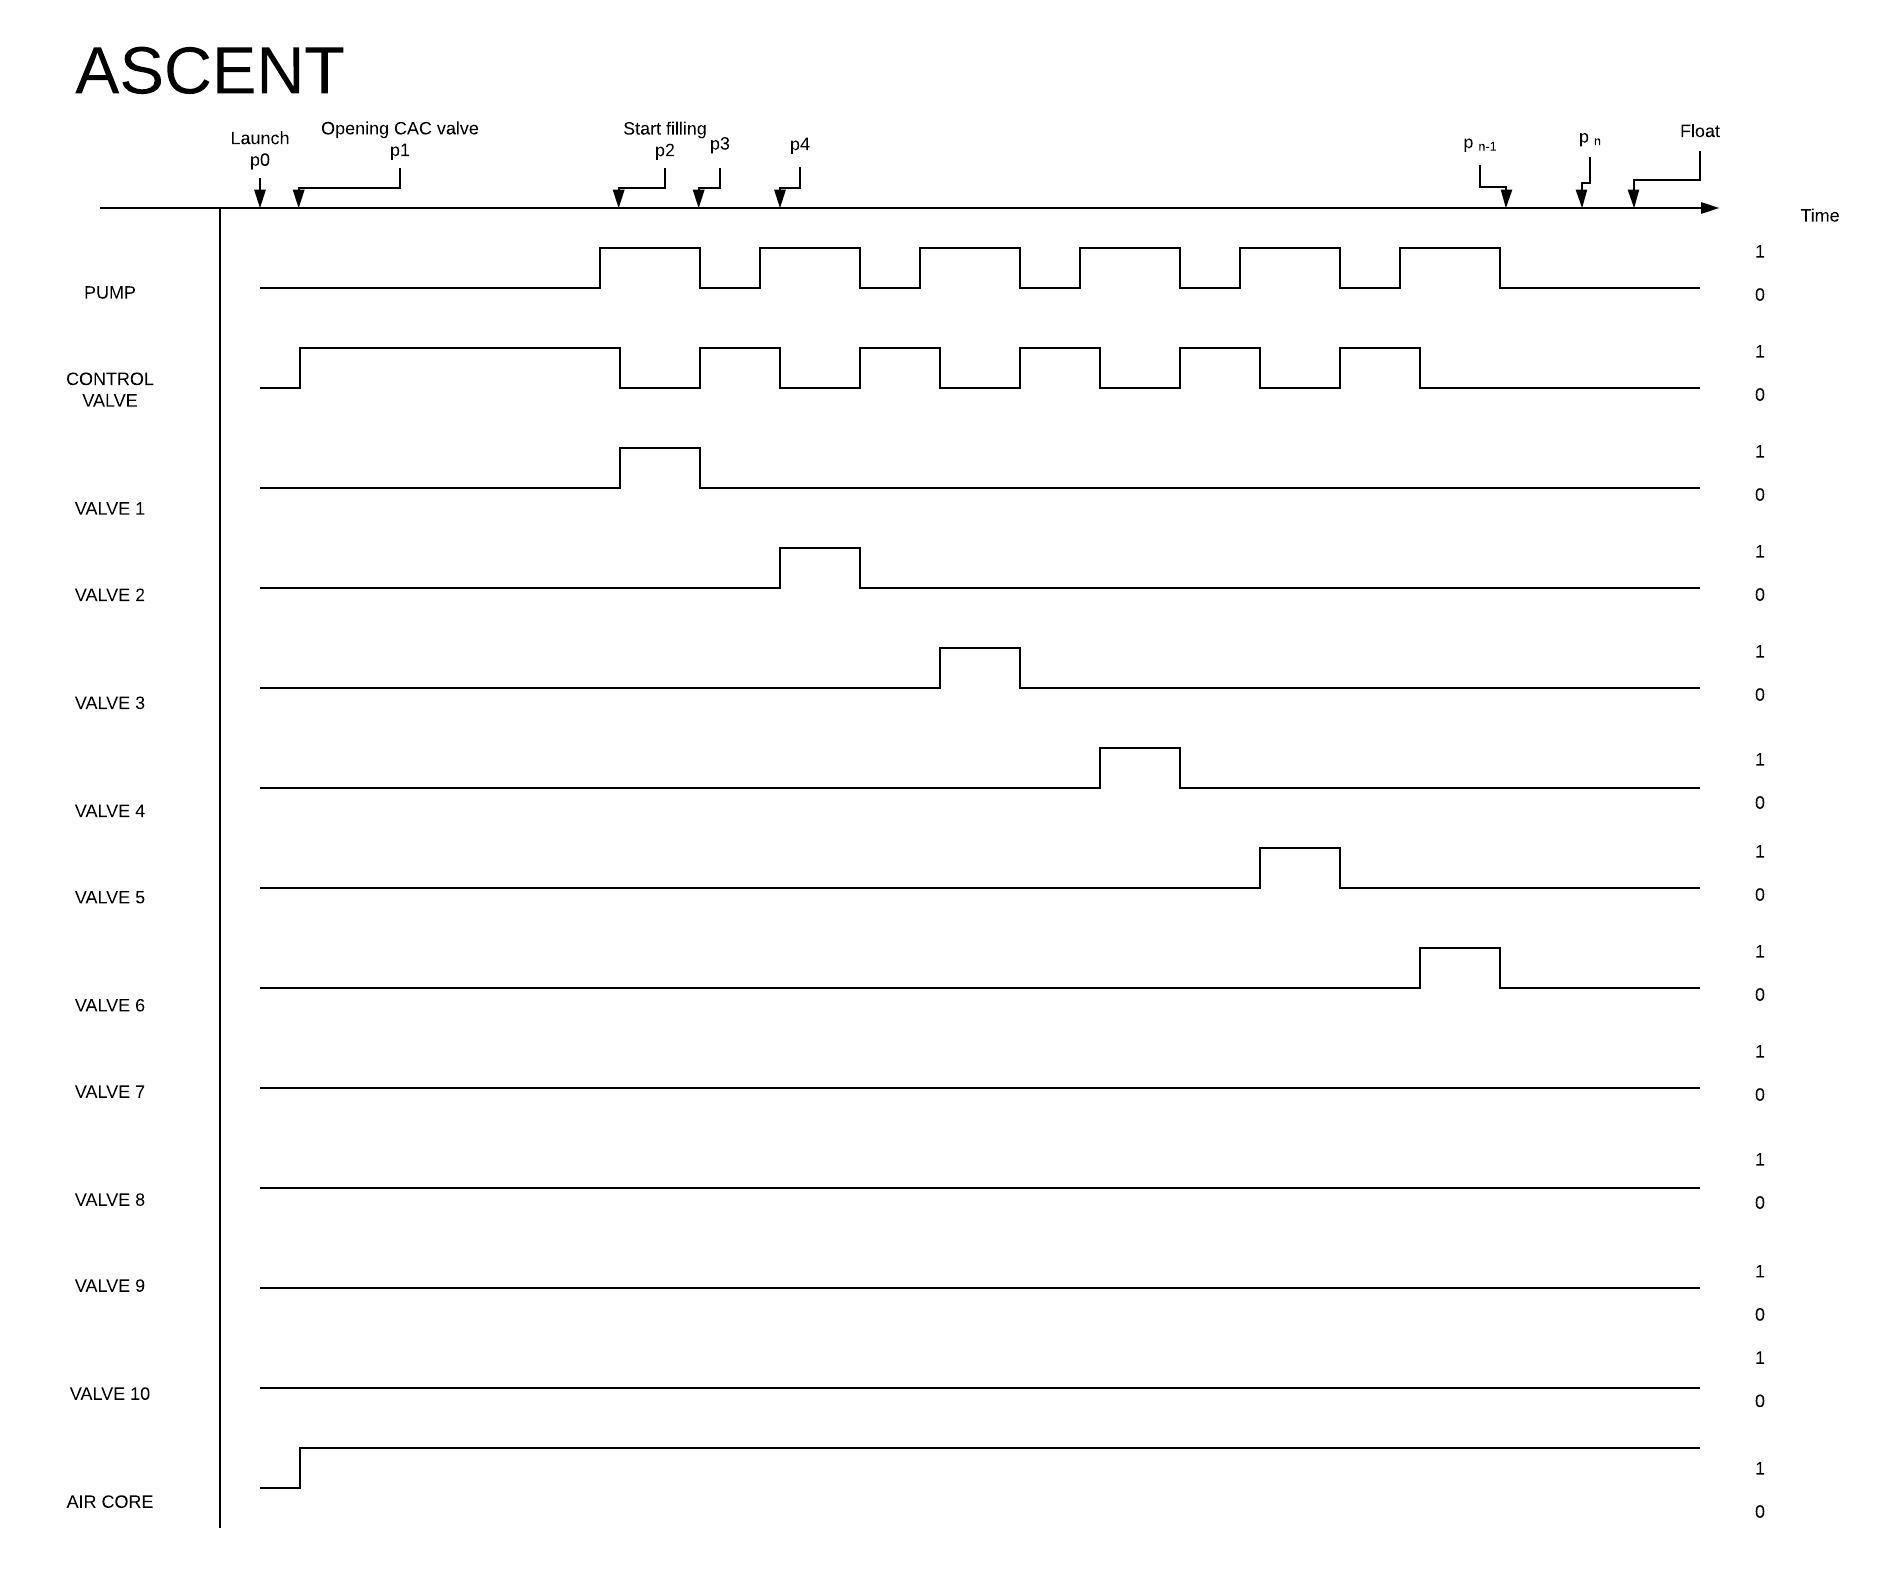
\includegraphics[width=1\linewidth]{4-experiment-design/img/ascent-phase.jpeg}
    \end{align*}
    \caption{The emptying and sampling sequence-Ascent Phase\label{fig:ascent}}
\end{figure}

\begin{figure}[H]
    \begin{align*}
        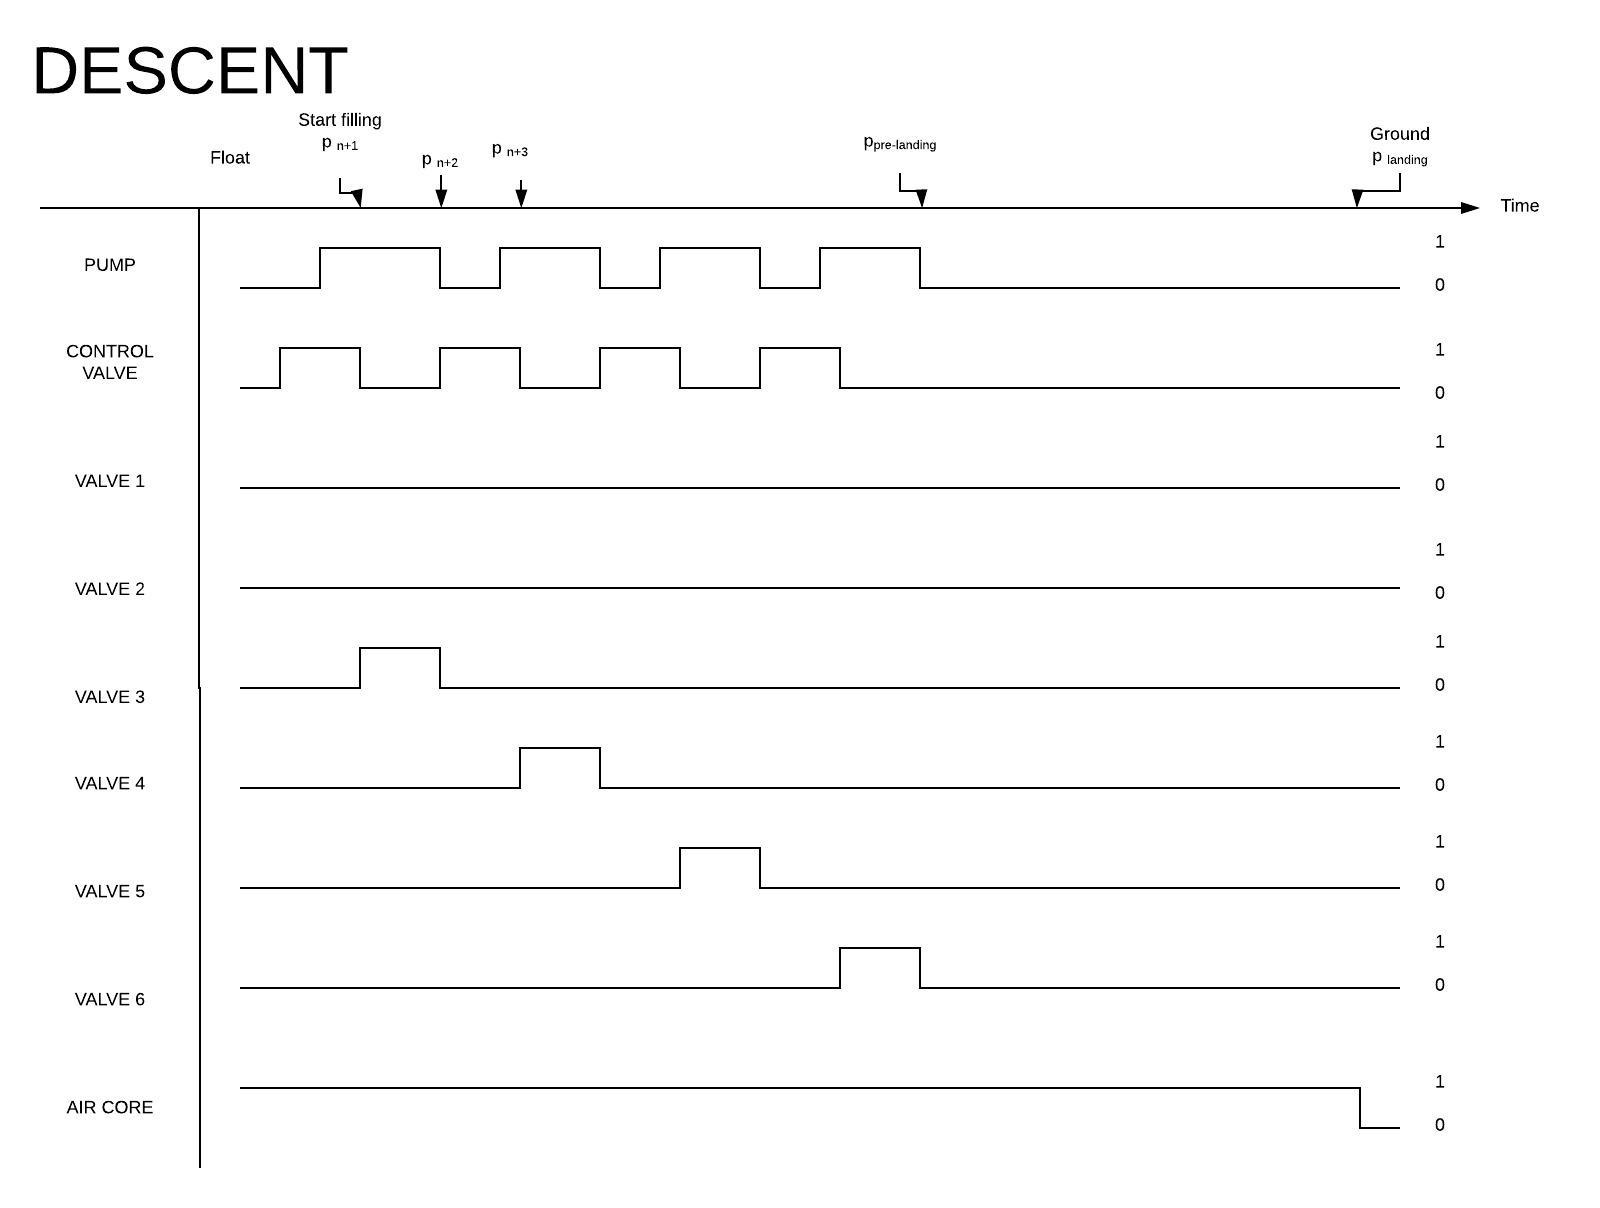
\includegraphics[width=1\linewidth]{4-experiment-design/img/descent-phase.jpeg}
    \end{align*}
    \caption{The emptying and sampling sequence-Descent Phase\label{fig:descent}}
\end{figure}

In the diagrams, 0 denotes closed/off and 1 denotes opened/on.

The general timeline of the experiment is as follow:

\textbf{Ascent Phase:}\\
$p_0$ – $p_1$
\begin{itemize}
    \item CAC valve shall be closed.
    \item AAC valves shall be closed.
    \item AAC' control valve shall be closed.
    \end{itemize}
$p_1$ – $p_2$
\begin{itemize}
    \item CAC valve shall be opened.
    \item AAC valves shall be closed.
    \item CAC tube shall be flushed.
    \item AAC' control valve shall be open.
    \end{itemize}
$p_2$ – $p_3$
\begin{itemize}
    \item Sampling bags' control valve shall be closed.
    \item Sampling bag valve 1 shall be opened, allowing for air to enter the first bag.
    \item CAC valve remains open.
    \end{itemize}
$p_3$ – $p_4$
\begin{itemize}
    \item Sampling bag valve 1 shall be closed
    \item Sampling bags' control valve shall be opened, allowing the system to flush. 
    \end{itemize}
$p_4$ - $p_n$
\begin{itemize}
    \item The above procedure shall repeat itself until the remaining one bag has collected air sample for its assigned altitude.
    \end{itemize}



\textbf{\\Float Phase:}\\
No action taken other than continued telemetry.
\begin{itemize}
    \item Sampling bag valve 2 shall be closed.
    \item Sampling bags' control valve shall be closed.
    \item Air pump is off.
\end{itemize}
 
\textbf{Descent Phase:}

Note: Before sampling starts again, the system has to be flushed. 

$p_{n+1}$ – $p_{n+2}$
\begin{itemize}
    \item Sampling bags' control valve shall be closed.
    \item Sampling bag valve 3 shall be opened, allowing for air to enter the first bag.
\end{itemize}

$p_{n+2}$ – $p_{n+3}$
\begin{itemize}
    \item Sampling bag valve 3 shall be closed
    \item Sampling bags' control valve shall be opened, allowing the system to flush. 
\end{itemize}

In between, same procedure shall repeat itself until all the remaining bags have collected air samples for their assigned altitudes.

$p_{pre-landing}$ 
\begin{itemize}
    \item System Sampling bag valve 6 shall be closed.
    \item Sampling bags' control valve shall be closed
    \item CAC valve shall be opened.
\end{itemize}


$p_{landing}$
\begin{itemize}
    \item CAC valve shall be closed.
\end{itemize}


Note: The AAC system's air pump is only on during sampling into the air sampling bags and flushing of the system.


\raggedbottom
\pagebreak
\subsection{Experiment Interfaces}

\subsubsection{Mechanical Interfaces}
\label{sec:4.2.1}

\bigskip
\begin{table}[H]
\noindent\makebox[\columnwidth]{%
\scalebox{0.8}{
\begin{tabular}{|c|c|c|c|c|c|}
\hline
\textbf{Component} & \textbf{Interface} & \textbf{Amount} & \textbf{Dimensions} &  \begin{tabular}[c]{@{}c@{}}\textbf{Total}\\ \textbf{weight}\end{tabular}  \\ \hline
Bracket standard 20/20 slot 6/6 & AAC-Gondola & $8$ & $20 \times 20 \times 20\ mm$ & $40\ g$ \\ \hline
Tolerance holes bracket & CAC-Gondola & $2$ & $ 20 \times 30 \times 52 \ mm$ & $50\ g$ \\ \hline
4-hole plate & AAC-CAC & $6$ & $1 \times 60 \times 45\ mm$ & $100\ g$ \\ \hline
Rubber bumpers M6 & AAC-Gondola, CAC-Gondola & $10$ & $19 \times 19 \times 15\ mm$ & $300\ g$ \\ \hline
T-nut slot 6 M4 & AAC-CAC, AAC-Gondola, CAC-Gondola & $44$ & $4 \times 5.9 \times 11.5\ mm$ & $132\ g$ \\ \hline
T-nut slot 8 M6 & AAC-Gondola, CAC-Gondola & $10$ & $6 \times 11 \times 16\ mm$ &  $60\ g$ \\ \hline

Steel bolt M4 & AAC-CAC, AAC-Gondola & $44$ & $8\ mm $ length & $34\ g$ \\ \hline
Steel washer M4 & AAC-CAC, AAC-Gondola & $24$ &\begin{tabular}[c]{@{}c@{}}$ID=4.3\ mm$\\ $OD=9\ mm$\end{tabular} &  $4.8\ g$\\ \hline
% Polyamide bolt M4 & Styrofoam-CAC-AAC & $8$ & $20\ mm $ length & $3\ g$ & $24\ g$ \\ \hline
% Polyamide washer M4 & Styrofoam-CAC-AAC & $8$ &\begin{tabular}[c]{@{}c@{}}$ID=4.3\ mm$\\ $OD=25\ mm$\end{tabular} & $4\ g$ & $32\ g$\\ \hline
Styrofoam bars  & AAC-Gondola, CAC-Gondola & $4$ & see Appendix \ref{sec:mech_drawings} & $450\ g$ \\ \hline
Handles  & CAC \& AAC & $4$ & $ 18.6 \times 25.2 \times 112.5 \ mm$ & $80\ g$ \\ \hline
\end{tabular}}}
\caption{Summary of Gondola-AAC-CAC Interfaces Components.}
\label{table:attaching-components}
\end{table}


\underline{Gondola - TUBULAR joining}

\smallskip
The experiment box will be fixed to the gondola rails by means of $10$ brackets interfacing the experiment outside structure with the hammer nuts in the rails. Two different types of brackets are used to be flexible with respect to the gondola rails distances, which can be modified by use after previous BEXUS campaigns. Eight small $20/20$ brackets (Figure \ref{fig:bracket_small}) are used to fix the AAC box to specific rails placement, and two other big brackets (Figure \ref{fig:bracket_big}) are used to fix the CAC box to the nearest rail. This method is secure as well as fast enough to provide an accessible and easy recovery for later analysis.

\begin{figure}[H]
    \noindent\makebox[\textwidth]{%
    \begin{subfigure}{.3\textwidth}
        \centering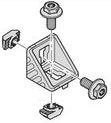
\includegraphics[width=0.55\textwidth]{4-experiment-design/img/Mechanical/bracket.jpg}
        \caption{Rexroth 20/20.}
        \label{fig:bracket_small}
    \end{subfigure}
    \hspace{1cm}
    \begin{subfigure}{.3\textwidth}
        \centering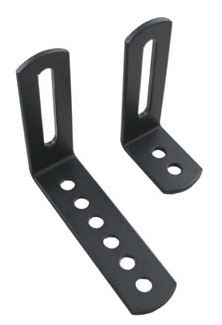
\includegraphics[width=0.55\textwidth,angle=90] {4-experiment-design/img/Mechanical/long_hole_bracket.jpg}
        \caption{Tolerance Holes.}
        \label{fig:bracket_big}
    \end{subfigure}}
    \caption{Bracket Components.}
    \label{fig:bracket}
\end{figure}

\bigskip
\underline{CAC - AAC joining}

\smallskip
A simple but reliable fixing interface between the two boxes of the experiment has been designed to ensure the fast recovery of the CAC box. The latter requires only unscrewing 12 bolts as well as unplugging a D-Sub connector marked in RED, see Figure \ref{fig:electrical_interfaces}. Once the CAC box is detached, the AAC Box will still remain perfectly fixed in the gondola. Table \ref{table:attaching-components} includes all the components required to fix the experiment to the gondola.

\bigskip
\underline{Handles}

\smallskip
Four top handles, as shown in Figure \ref{fig:handles} will be mounted to facilitate the experiment box manipulation when moving it in and out of the gondola.

\begin{figure}[H]
    \centering
    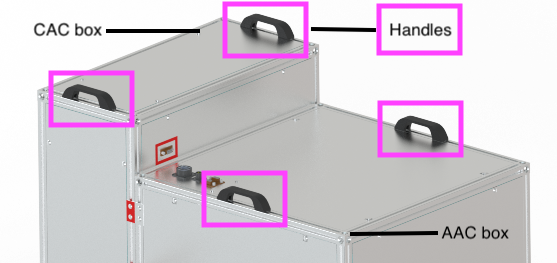
\includegraphics[width=0.8\textwidth]{4-experiment-design/img/Mechanical/Figure_8.png}
    \caption{Handling Interfaces.}
    \label{fig:handles}
\end{figure}

\bigskip
\underline{Inlet/Outlet Pipes}
\label{subsec:pipes}

\smallskip
In order to collect reliable air samples, the experiment requires to be mounted with at least one side exposed to the outside. This will reduce the pipe length used to collect clean air. As it can be seen in Figure \ref{fig:3D_tubular_render}, three pipes will extend from the experiment box face: one for the CAC sampling and two, input and output, for the AAC sampling. 

These pipes are welded/drawn $304$ grade stainless steel tubes from RESTEK company, which are specially recommended for chromatography applications and gas delivery systems with low pressures and inert environments. These tubes are sulfinert, which is a required treatment for metal components when analyzing for parts-per-billion levels of organo-sulfur compounds.

The tubes, which are the same that will be used in the pneumatic system of the \emph{Brain} (see Section \ref{sec:4.4.5}), have an outer diameter $OD = 6.35\ mm$ ($1/4$ inches) and an inner diameter $ID = 4.57\ mm$ ($0.18$ inches).

\bigskip
\underline{Pump vibration}
\label{subsec:vibration}

To mitigate the vibrations produced by the pump, an extra piece of styrofoam has been added between the pump's anchor plate and the surface of the level 1 of the brain, where this key component is fixed. 


\subsubsection{Thermal Interfaces}
\label{sec:4.2.2}

Both main structural components and external walls of the two boxes of the experiment are made by aluminum and steel components. For this reason, since these are conductive materials, a direct attachment to the gondola creates many heat paths with the internal space and subsystems of the experiment. Considering that the temperature gradient between the gondola and the operative requirements of the electronic components can be quite high, this conductive connections drastically decrease the efficiency of the thermal insulation. Therefore, a system based on rubber bumpers and styrofoam bars (see Figure \ref{fig:thermal_interface}) has been designed to remove heat bridges and minimize temperature leaks from the inside of the experiment to the outside.

Figure \ref{fig:rubber_bumper} shows a CAD model of the bumper component and how it looks like when attached to the gondola with the brackets explained in the previous section.

\begin{figure}[H]
    \noindent\makebox[\textwidth]{%
    \begin{subfigure}{.3\textwidth}
        \centering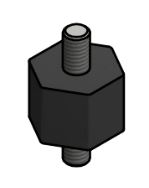
\includegraphics[width=0.55\textwidth]{4-experiment-design/img/Mechanical/rubber_bumper.jpg}
    \end{subfigure}
    \hspace{1cm}
    \begin{subfigure}{.3\textwidth}
        \centering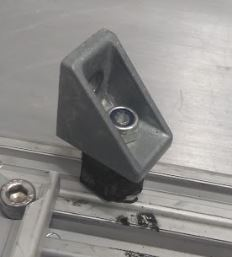
\includegraphics[width=0.55\textwidth] {4-experiment-design/img/Mechanical/real_bumper.jpg}
    \end{subfigure}}
    \caption{Rubber Bumper.}
    \label{fig:rubber_bumper}
\end{figure}

The styrofoam bars will be attached directly to the rails of the experiment structure by M4 plastic screws and big washers.

\begin{figure}[H]
    \centering
    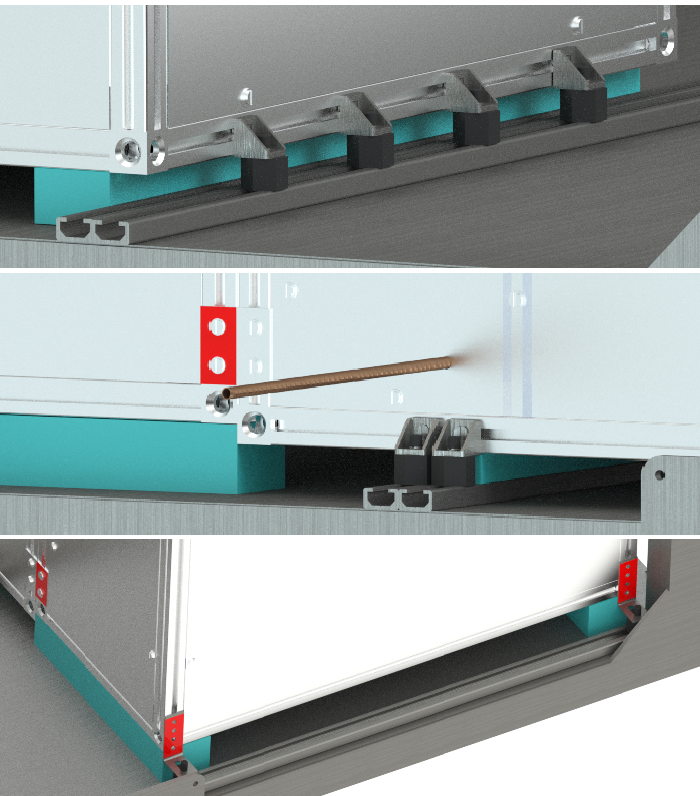
\includegraphics[width=0.6\textwidth]{4-experiment-design/img/Mechanical/gondola_fixation.png}
    \caption{Thermal Interfaces TUBULAR-Gondola.}
    \label{fig:thermal_interface}
\end{figure}

\subsubsection{CAC Interfaces}
An uncoupled quick connector, shown in Figure \ref{fig:Quick-connector-body}, will be attached at each end of the coiled tube to seal the opening. It will remain tightly sealed until the quick connectors are manually coupled. 

\begin{figure}[H]
    \centering
    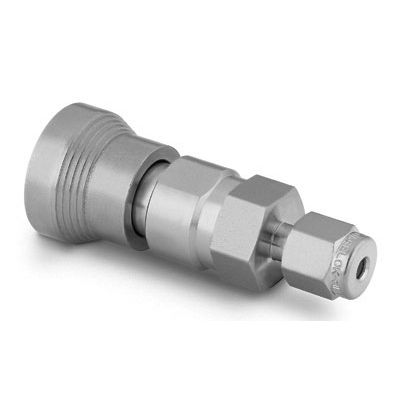
\includegraphics[width=0.2\textwidth]{4-experiment-design/img/Mechanical/CAC-QC-Outlet.jpg}
    \caption{Swagelok Quick Connector Body.}
    \label{fig:Quick-connector-body}
\end{figure}

The interfaces between the other parts in the CAC set up will be joined with specific tube fittings, listed in Table \ref{tab:CAC-interfaces}. All the chosen interfaces are from Swagelok. Using products from the same manufacture minimizes the risk for leakage or mismatched interfaces in the system. 

\begin{table}[H]
\centering
\scalebox{0.8}{
\begin{tabular}{|c|c|c|c|}
\hline
\textbf{Component}                                                          & \textbf{Interface}             & \textbf{Amount} & \textbf{Fitting Size}                                                    \\ \hline
\begin{tabular}[c]{@{}c@{}}Quick connector body\\ SS-QC4-B-200\end{tabular} & Outlet of coiled tube          & 1               & 1/8 in.                                                                  \\ \hline
\begin{tabular}[c]{@{}c@{}}Quick connector body\\ SS-QC4-B-400\end{tabular} & Inlet of coiled tube           & 1               & 1/4 in.                                                                  \\ \hline
\begin{tabular}[c]{@{}c@{}}Quick connector stem\\ SS-QC4-D-400\end{tabular} & Inlet of coiled tube -  Filter & 1               & 1/4 in.                                                                  \\ \hline
\begin{tabular}[c]{@{}c@{}}Male connector\\ SS-400-1-2\end{tabular}             & Tube fitting - Solenoid valve   & 2               & \begin{tabular}[c]{@{}c@{}}Tube OD 1/8 in. to \\ Tube OD 1/4 in.\end{tabular}    \\ \hline
\begin{tabular}[c]{@{}c@{}}Straight Tube Union\\ SS-200-6\end{tabular}             & Quick connector 1/8 in. - Tube 1/8 in.     & 1               & 1/8 in.
\\ \hline
\begin{tabular}[c]{@{}c@{}}Tube Reducer\\ SS-400-6-2 \end{tabular}             & Tube 1/8 in. - Tube 1/4 in.     & 1               & \begin{tabular}[c]{@{}c@{}}Tube OD 1/8 in. to \\ Tube OD 1/4 in.\end{tabular}
\\ \hline
\begin{tabular}[c]{@{}c@{}}Straight Tube Union\\ SS-400-6\end{tabular}             & Tube 1/4 in. - 90 degree connector    & 1               & 1/4 in.
\\ \hline
\begin{tabular}[c]{@{}c@{}}Union 90-degree connector\\ SS-400-9\end{tabular}             &
\begin{tabular}[c]{@{}c@{}} Between certain tube fittings\\ Outlet tube \end{tabular} & 3               & 1/4 in.
\\ \hline
\begin{tabular}[c]{@{}c@{}}Tube fitting\\ SS-401-PC\end{tabular}             & \begin{tabular}[c]{@{}c@{}} Between certain tube fittings\\ Magnesium dryer filter \end{tabular} & 5               & 1/4 in.
\\ \hline
\end{tabular}}
\caption{Interfaces within CAC Setup.}
\label{tab:CAC-interfaces}
\end{table}

\subsubsection{AAC Interfaces}
In the AAC system, the interfaces between various components are a mixture of eleven different types of tube fittings from Swagelok. The selected types are straight and elbow union, T-union, female and male elbows, male and female connectors, tube fittings, and quick coupling with a certain  specifications. Some of them are shown in Figure \ref{fig:AAC-interfaces-fittings}. Information regarding the fitting's placement in the AAC and fitting sizes are summarized in Table \ref{tab:AAC-interfaces}. 

\begin{figure}[H]
    \centering
    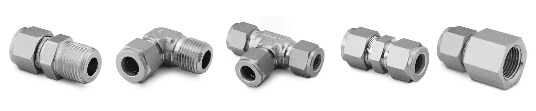
\includegraphics[width=0.8\textwidth]{4-experiment-design/img/Mechanical/AAC-interfaces.jpg}
    \caption{From Left to Right: Male Connector, Male Elbow, T-union, Straight Union and Female Connector.}
    \label{fig:AAC-interfaces-fittings}
\end{figure}

\begin{table}[H]
\centering
\scalebox{0.9}{
\begin{tabular}{|c|c|c|c|}
\hline
\textbf{Component}                                                    & \textbf{Interface}                                                                                                                                                                         & \textbf{Amount} & \textbf{Fitting Size}                                                                     \\ \hline
\begin{tabular}[c]{@{}c@{}}Male connector\\ SS-400-1-2\end{tabular}   & \begin{tabular}[c]{@{}c@{}}Airflow sensor - Sensor box\\ Tube sensor box - Manifold \\ Manifold - Flushing valve\\ Flushing valve - Outlet tube\\ Solenoid valve - Tube valve\end{tabular} & 11              & \begin{tabular}[c]{@{}c@{}}Male 1/8 in. to \\ Tube OD 1/4 in.\\ ID 0.21 in.\end{tabular}  \\ \hline
\begin{tabular}[c]{@{}c@{}}Male elbow\\ SS-400-2-2\end{tabular}       & Sensor box - Tube sensor box                                                                                                                                                               & 1               & \begin{tabular}[c]{@{}c@{}}Male 1/8 in. to \\ Tube OD 1/4 in.\\ ID 5/32 in.\end{tabular}  \\ \hline
\begin{tabular}[c]{@{}c@{}}Straight union\\ SS-400-6\end{tabular}     & \begin{tabular}[c]{@{}c@{}}Filter - Tube filter\\ Tube filter - Pump\\ Pump - Tube pump\end{tabular}                                                                                       & 3               & \begin{tabular}[c]{@{}c@{}}Tube OD 1/4 in.\\ ID 5/32 in.\end{tabular}                     \\ \hline
\begin{tabular}[c]{@{}c@{}}Female connector\\ SS-400-7-4\end{tabular} & \begin{tabular}[c]{@{}c@{}}Inlet tube - Filter\\ Tube pump - Airflow sensor\\ Airflow sensor - Tube airflow sensor\end{tabular}                                                            & 3               & \begin{tabular}[c]{@{}c@{}}Female 1/4 in. to\\ Tube OD 1/4 in.\\ ID 5/32 in.\end{tabular} \\ \hline
\begin{tabular}[c]{@{}c@{}}T-Union\\ SS-400-3\end{tabular}            & Tube valve - Bag valve                                                                                                                                                                     & 6               & Male 1/4 in.                                                                              \\ \hline
\end{tabular}}
\caption{Interface Descriptions Inside AAC System.}
\label{tab:AAC-interfaces}
\end{table}


\subsubsection{Electrical Interfaces}
\label{sec:4.2.3}

The experiment will connect to the gondola electrically via a 4 pin, male, box mount receptacle MIL - C-26482P series 1 connector with an 8-4 insert arrangement (MS3112E8-4P) \cite{BexusManual}. It will connect to one 28.8 V/1 mA battery pack which consists of eight SAFT LSH20 batteries in series where each has a 5 A fuse\cite{BexusManual}. The expected maximum current is 1.1 A.

\begin{figure}[H]
    \centering
    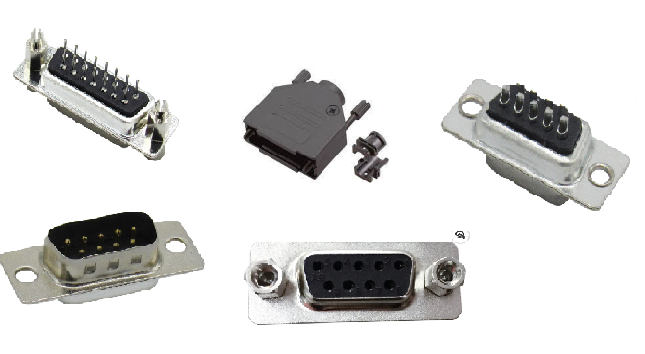
\includegraphics[width=0.4\textwidth]{4-experiment-design/img/connectors.png}
    \caption{Connectors.}
    \label{fig:connectors}
\end{figure}

The E-Link connection shall be made between the experiment and the E-Link system using a RJ45 connection which will be supplied by SSC and an Ethernet protocol. The Amphenol RJF21B connector will be mounted on either the front or the side of the experiment\cite{BexusManual}.  

The CAC and AAC will be connected together with a D-SUB 9-pin connector where power, ground and signals for the sensors in the CAC will be connected. A female connector will be located on the AAC wall and a male connector on the CAC wall.

Another female D-SUB 9-pin connector will be located on the wall of the AAC in which the connections for the three ambient pressure sensors will be located. Connectors with different pin configuration are shown in Figure \ref{fig:connectors}.

The expected data rate is 1.58 kbits/s for downlink and 1.08 kbits/s for uplink.

\begin{figure}[H]
    \centering
    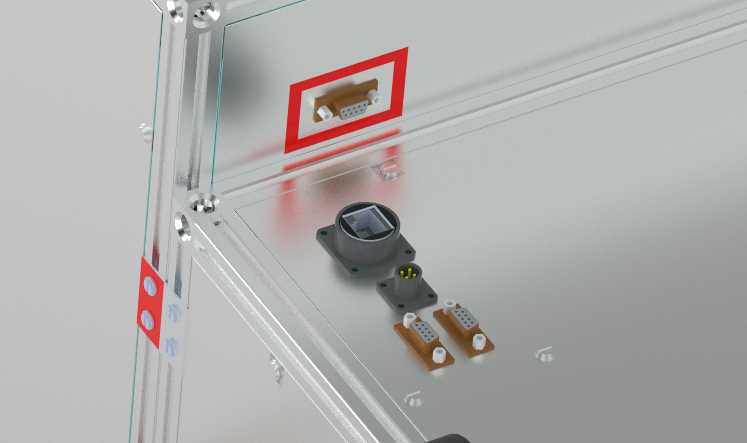
\includegraphics[width=0.8\textwidth]{4-experiment-design/img/Mechanical/Figure_Detail_Interfaces.png}
    \caption{Electrical Interfaces.}
    \label{fig:electrical_interfaces}
\end{figure}



%\begin{figure}[H]
%    \begin{align*}
%        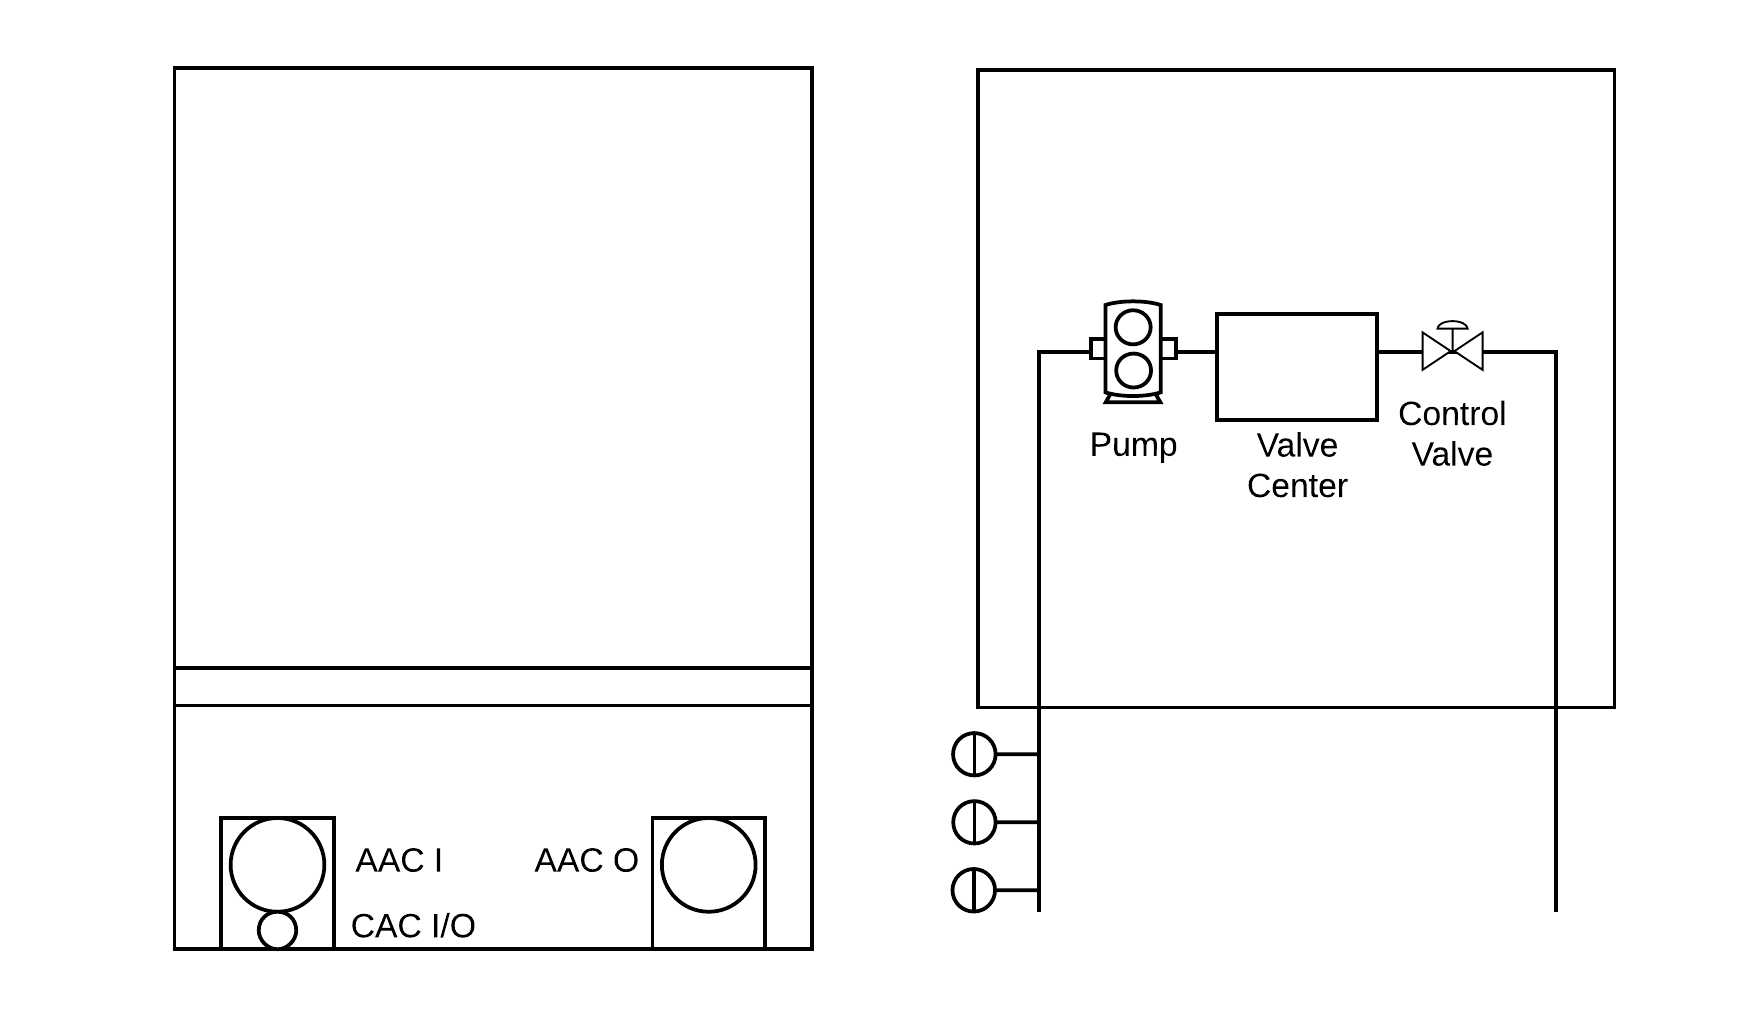
\includegraphics[width=0.7\textwidth]{4-experiment-design/img/Diagram_pipe.png}
%    \end{align*}
%    \caption{Diagram of the experiment box face exposed to the outside.}\label{fig:pipes_interface_1}
%\end{figure}

\iffalse
\subsubsection{Radio Frequencies (Optional)}
\begin{centering}
Not required.
\end{centering}
\bigskip

\subsubsection{Thermal (Optional)}
\begin{centering}
Not required.
\end{centering}
\bigskip
\fi


\raggedbottom
\begin{landscape}
\subsection{Experiment Components}
\subsubsection{Electrical Components}

Table \ref{tab:electrical-components} shows all required electrical components with mass and price.

%


\begin{longtable}{|m{0.03\textwidth}|m{0.3\textwidth}|m{0.25\textwidth}|m{0.05\textwidth}|m{0.1\textwidth}|m{0.3\textwidth}|m{0.15\textwidth}|m{0.08\textwidth}|}
    
\hline
\textbf{ID} & \textbf{Components} & \textbf{Specs (size,weight)} & \textbf{No.} & \textbf{Cost} & \textbf{Note} & \textbf{Availability} & \textbf{Status} \\ 
\hline
1 & Arduino Due & 101.52 mm x 53.3 mm, 36 g & 1 & 35 Euro & Fast and has many analog, and digital pins & Easily ordered online & Ordered \\ \hline
2 & W5500 Ethernet Shield  & 36 g & 1 & 28 Euro & Easily, connected on top of the board & Easily ordered online & Ordered \\ \hline
3 & KNF 850.1.2. KNDC B Miniature Diaphragm Pump & 30 x 54.3 x 77.5 mm, 430g  & 1 & 350 Euro & Low power, small size & Ordered online & Ordered \\ \hline
4 & Barometric Pressure Sensor MS5607-02BA03 & 5.0 x 3.0 x 1.0 mm, 1g  & 3 &  11 Euro & High resolution, large measuring range & Easily ordered online & To be ordered online \\ \hline
5 & Electromagnetically controlled valve & 1-1/2", 2640 g & 12 & 1756 Euro & Cascaded/series of valves & Easily ordered online & One ordered for testing \\ \hline
6 & Airflow sensor AWM40000 Series & 14 g & 1 & 106 Euro & good temperature range, high accuracy & Easily ordered online & To be ordered online \\ \hline
7 & Polyimide Thermofoil Heaters HK5161R78.4L12 & 12.7 x 101.6 mm, 6.84g & 1 & 40 Euro & Easy to mount, compact size & Easily ordered online & To be ordered online \\ \hline
8 & Polyimide Thermofoil Heaters HK5160R157L12 & 12.7 x 50.8 mm, 6.84g & 1 & 40 Euro & Easy to mount, compact size & Easily ordered online & To be ordered online \\ \hline
9 & Temperature sensor VSSOP-8, LM75A, Texas Instruments & 5.3 x 3.4 x 1.4 mm & 12 & 4 Euro & I2C digital output interface, temperature range down to - 55 ℃ & Easily ordered online & To be ordered online \\ \hline
10 & DC-DC Converter TEN 5 Series, 6 W, 12 V & 20.3 x 31.8 mm, 33.8 g & 3 & 50 Euro & Provides required output voltage and power & Easily ordered online & To be ordered online \\ \hline
11 & HDC2010 Low Power Humidity Digital Sensors & 1.5 x 1.5 x 0.675 mm, 15g & 1 & 3 Euro & I2C interface, good temperature range, high accuracy & Easily ordered online & To be ordered online \\ \hline
12 & Industrial temperature microSD XCUHS-I 8GB & 15 x 11 x 1 mm, 0.5 g & 1 & 20 Euro & Small, good temperature range, sufficient storage & Easily ordered online & Ordered  \\ \hline
13 & Logic CAT5E Network (2m) & 2 m, 90g & 1 & 7 Euro & Will be used for testing & Easily ordered in the nearest store & To be bought \\ \hline
14 & Electrical wires & 30g &  30 & 15 Eur & For use in testing and the final PCB board and circuitry & Easily ordered online & To be ordered \\ \hline
15 & Heat sinks & 25g &  5 &  5 Eur & For dissipating heat generated from components & Easily ordered online & To be ordered \\ \hline
16 & Resistors & 15g & 3 & 1.5 Eur & For use in valve switching circuit & Easily ordered online & To be ordered \\ \hline
17 & Transistors & 18g & 18 & 9 Eur &  For use in valve switching circuit & Easily ordered online & To be ordered \\ \hline 


    \caption{Table showing all required electrical components}
    \label{tab:electrical-components}
\end{longtable}
\raggedbottom

\begin{table}[H]
    \begin{align*}
        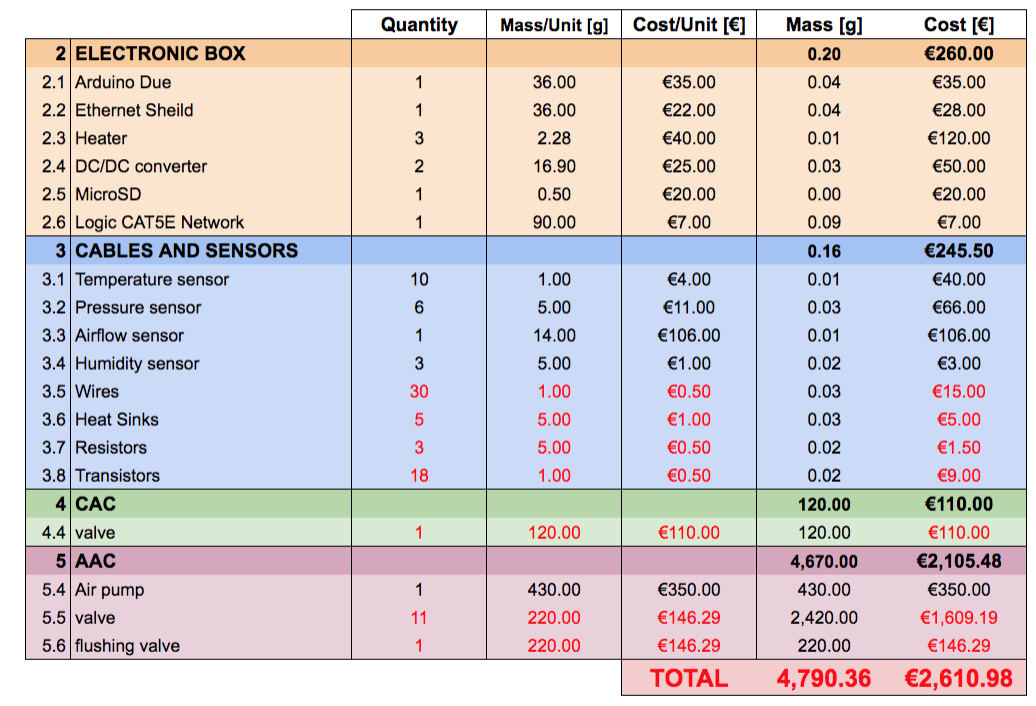
\includegraphics[height=10cm]{4-experiment-design/img/electrical-components-table.png}
    \end{align*}
    \caption{Table showing all required electrical components.}\label{tab:electrical-components}
\end{table}

\end{landscape}

\begin{landscape}

\subsubsection{Mechanical Components}

Table \ref{tab:mechanical-components} shows all required mechanical components with mass and price. Table cells highlighted in yellow denote values that have yet to be determined.

%\begin{longtable}{|m{0.03\textwidth}|m{0.2\textwidth}|m{0.25\textwidth}|m{0.05\textwidth}|m{0.1\textwidth}|m{0.28\textwidth}|m{0.15\textwidth}|m{0.15\textwidth}|}
     
   
\hline
\textbf{ID} & \textbf{Components} & \textbf{Specs (size,weight)} & \textbf{No.} & \textbf{Cost} & \textbf{Note} & \textbf{Availability} & \textbf{Status} \\ \hline
1 & Aluminum Bar & 45cm & 16 & TBD\footnote{Request for quotes have been sent to identified vendors and responses are still pending. \label{fn:mechcomp1}} & Railed geometry, Structural element & Online & To be ordered \\ \hline
2 & Aluminum Bar & 40cm & 4 & TBD\textsuperscript{\ref{fn:mechcomp1}} & Railed geometry, Structural element & Online & To be ordered \\ \hline
3 & Aluminum Bar & 25cm & 4 & TBD\textsuperscript{\ref{fn:mechcomp1}} & Railed geometry, Structural element & Online & To be ordered \\ \hline
4 & Aluminum Plate & 50 x 40 x 0.2 cm & 4 & TBD\footnote{The other elements still need to be found either in the store or online. \label{fn:mechcomp2}} & Wall, Protective element & Store & To be ordered \\ \hline
5 & Aluminum Plate & 50 x 25 x 0.2 cm & 4 & TBD\textsuperscript{\ref{fn:mechcomp2}} & Wall, Protective element & Store & To be ordered \\ \hline
6 & Aluminum Plate & 50 x 50 x 0.2 cm & 2 & TBD\textsuperscript{\ref{fn:mechcomp2}} & Wall, Protective element & Store & To be ordered \\ \hline
7 & Styrofoam & 2 $m^2$, 2.5cm thick & 1 & TBD\textsuperscript{\ref{fn:mechcomp2}} & Wall, Protective element & Store & To be ordered \\ \hline
8 & Bag Valves & \textit{Swagelok} & 16 & TBD\textsuperscript{\ref{fn:mechcomp1}} & Interface bags with tubes & Online & To be ordered \\ \hline
9 & 90-degree angle & 0.25 x 0.25 cm & 52 & TBD\textsuperscript{\ref{fn:mechcomp2}} & Join structure bars & Online & To be ordered \\ \hline
10 & Coated box & 10 x 10 x 3 cm & 1 & TBD\textsuperscript{\ref{fn:mechcomp2}} & Valve center for AAC & Store & To be built \\ \hline
11 & Plastic Tube & 5 m & 1 & TBD\textsuperscript{\ref{fn:mechcomp2}} & Valves to bags & Store & To be ordered \\ \hline
12 & Air Filter & TBD\textsuperscript{\ref{fn:mechcomp2}} & 1 & TBD\textsuperscript{\ref{fn:mechcomp2}} & Main pipe protection & Store & To be built \\ \hline
13 & Flange & Small & 50 & TBD\textsuperscript{\ref{fn:mechcomp2}} & Join tubes with valves & Store & To be ordered \\ \hline
14 & Hinges & 5 x 5 x 0.1 cm & 2 & TBD\textsuperscript{\ref{fn:mechcomp2}} & Allow opening mechanism & Store & To be ordered \\ \hline
15 & Bar & 52.4 x 0.8 cm & 4 & TBD\textsuperscript{\ref{fn:mechcomp2}} & Anchor point fro bags & Store & To be ordered \\ \hline
16 & Handle & TBD\textsuperscript{\ref{fn:mechcomp2}} & 4 & TBD\textsuperscript{\ref{fn:mechcomp2}} & Experiment box manipulation & Store & To be ordered \\ \hline

    \caption{Table showing all required mechanical components}
    \label{tab:mechanical-components}
\end{longtable}
\raggedbottom

\begin{table}[H]
    \begin{align*}
        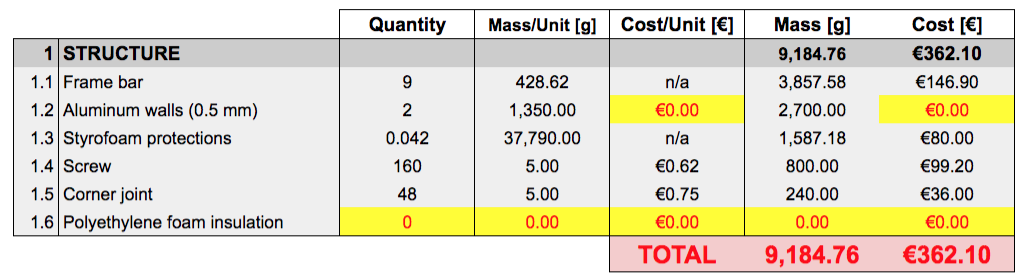
\includegraphics{4-experiment-design/img/mechanical-components-table.png}
    \end{align*}
    \caption{Table showing all required mechanical components.}\label{tab:mechanical-components}
\end{table}

\subsubsection{Other Components}

Other components are included in the full budget previously presented in Table \ref{tab:budget-table}.

\end{landscape}

\raggedbottom
\pagebreak
\subsection{Mechanical Design} \label{Mechanical_Design}


\subsubsection{Structure}

The experiment consists on two cubic boxes, one stacked next to the other. The smallest box allocates the heaviest element, the CAC. The main box contains the AAC system as well as the general Electronic Box (EB). The frame of these two boxes will be made of aluminum bars which have a characteristic cross-section of 20x20 mm, see Figure \ref{cross-section}. The rails will allow an easy interface between bars and other elements. Bars will be joined together by using 90-degree angles, see Figure \ref{3_bars_joined}.

%% Cross section of one aluminum bar

\begin{figure}[!ht]
    \centering
    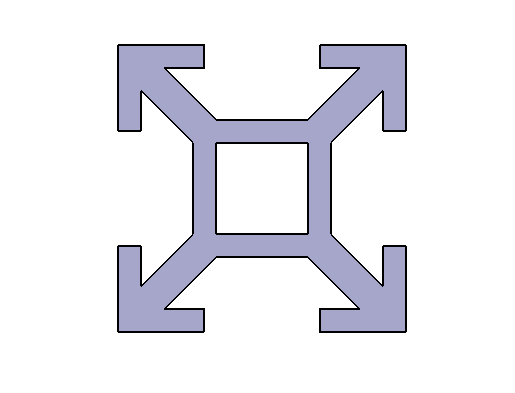
\includegraphics[width=0.5\textwidth]{4-experiment-design/img/1_cross_section.jpg}
    \caption{Cross section of the structural bars.}
    \label{cross-section}
\end{figure}

% Figure of 3 bars

\begin{figure}[!ht]
    \centering
    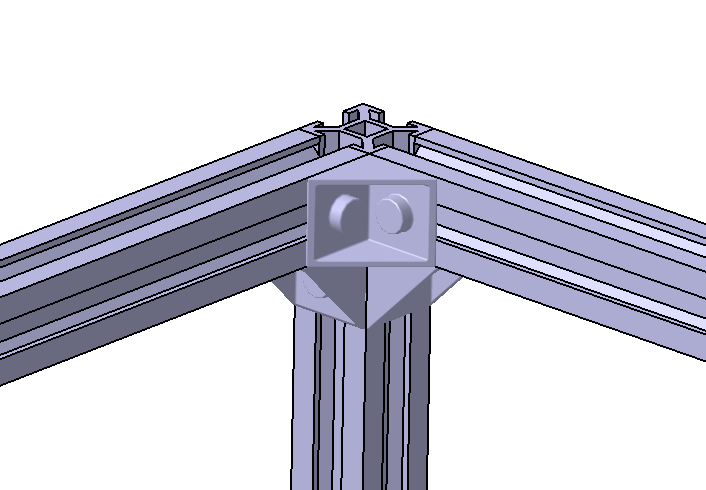
\includegraphics[width=0.6\textwidth]{4-experiment-design/img/bars_joint.jpg}
    \caption{Interface between structural bars.}
    \label{3_bars_joined}
\end{figure}

The frame is designed to withstand all vibrations and ensure a reliable stability of the entire system. Further tests will help to confirm and update the design if necessary. 

The two-box design will allow ease of access and manipulation of both the CAC and AAC subsystems, see Figure \ref{strucutre}. In addition, the AAC sampling system is designed to be re-usable for future handover to FMI, as such, it will be mountable on any standard balloon flight without having to introduce major design changes. The latter would imply to introduce a battery as a power unit, hence less bags could be carried (around 8 bags in the new setup).

% Figure of the two structures one above the other one (slightly separated)
\begin{figure}[!ht]
    \centering
    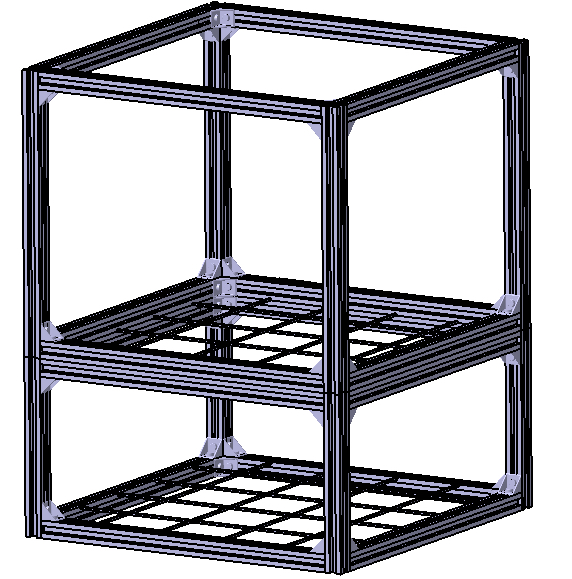
\includegraphics[width=0.7\textwidth, angle=90]{4-experiment-design/img/frame_structure.jpg}
    \caption{Structure of the two-box design.}
    \label{strucutre}
\end{figure}

\subsubsection{CAC Subsystem}

The CAC subsystem is designed with a 300-meter coiled tube, the valve governing it and a temperature sensor. To determine its positioning inside the gondola and the experiment box, some mechanical issues must be considered.

\smallskip
Firstly, it is possible to identify the interface to attach the experiment box to the gondola as one of the most critical points in terms of mechanics performance. In the worst case scenario, with a heavy experiment and without a proper study of the aforesaid interface, shear in the screws could be produced after a violent landing stress. Since the CAC will be the heaviest component in the whole experiment, its location and orientation will affect directly the stress analysis of the structure. The larger the distance to the fixed points, the bigger the Momentum produced by the component. Nevertheless, due to fast recovery implementation, the CAC tube will be placed vertically. Therefore, its dedicated box will be properly attached to the AAC box by means of 4 anchor points. The fast recovery then will only imply unscrewing 4 screws and disconnect a wire. 

\smallskip
In order to command the valve, a wire will go out from the box and plugged on the electronics interface panel located on an AAC box wall.

\smallskip
In addition, to avoid sample contamination with standstill air inside the gondola, the coil will have a direct outside inlet and outlet by means of an extension tube reaching further from the gondola’s limits.


\pagebreak
\subsubsection{AAC Subsystem}

The AAC Subsystem consists of 10 three-liter sampling bags. Each bag will have a dedicated valve in the Valve Center (VC) to allow emptying and filling processes as well as to close the bag when needed. The bags will be placed vertically and will have two anchor points: on the top through a  multiple anchor interface (see Figure \ref{anchor_bags}) and on the bottom by means of the tubes connecting them to the valves.

%% Several Figures of the top box with its inside elements: isometric, top view and front view.

\begin{figure}[!ht]
    \centering
    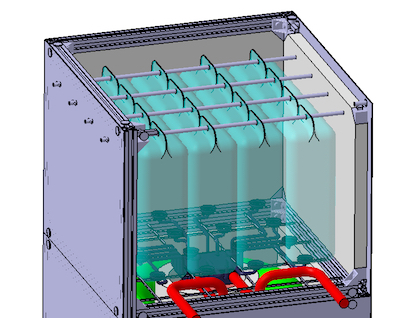
\includegraphics[width=0.7\textwidth]{4-experiment-design/img/anchored_bags.jpg}
    \caption{AAC Subsystem with all its elements.}
    \label{anchor_bags}
\end{figure}

\pagebreak
\subsubsection{Electronics Box}

The OBC and its external elements will be allocated in a bottom corner of the experiment box, inside AAC box, and on the opposite side of the CAC box. The latter will allow an easy access and manipulation as well as the required external interfaces. The smallest side of the EB will have the outer connections interfaces. Hence, the wall will have the necessary holes. The EB will be fixed to the AAC box structure bars in 3 different points.


%% Figure of the electronics box inside the coil, only bottom cube, isometric top view, explosion

%\begin{figure}[!ht]
 %   \centering
  %  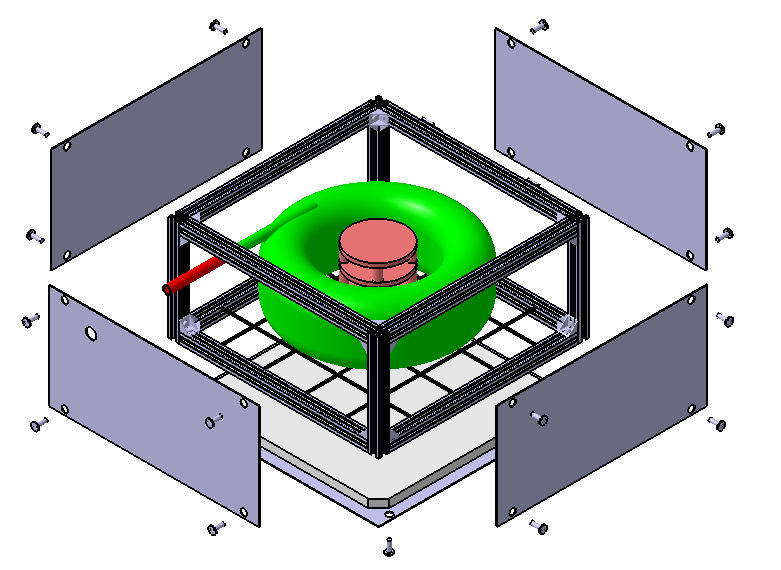
\includegraphics[width=0.7\textwidth]{4-experiment-design/img/explos_CAC.jpg}
   % \caption{.}
    %\label{electronics_box}
%\end{figure}

\pagebreak
\subsubsection{Valve Center}

The valve center consists of a coated box to which the AAC's 10 air sampling bags will be attached to. This box will serve as the air flow chamber. It will be connected to a pipe from which outside air will be pumped and also enable pre-sample collection flushing, see Figure \ref{valve_center_and_pipes}. The pump providing the airflow will be allocated on the inlet side and protected by an air filter. It will be allocated inside a shielding box, more detailed information in section \ref{Thermal_section}.

\smallskip
Both the pump box and the valve center will be allocated above the EB so all the command center is at the same place. Having them together will provide as well a proper cooling system monitored by several temperature sensors. A sketch of the setup can be seen in Figure ....

%% Figure of the valve center with the pipe and small tubes

%\begin{figure}[!ht]
%    \centering
%    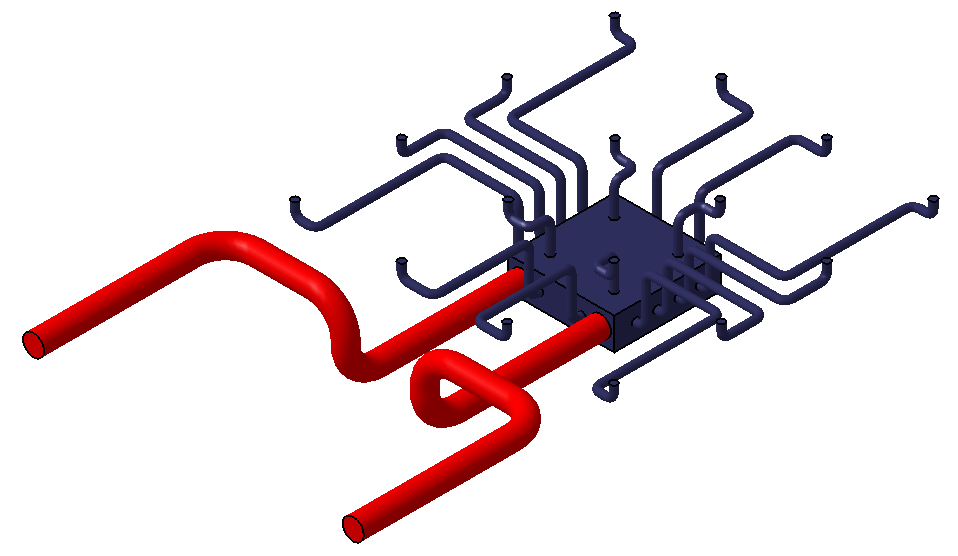
\includegraphics[width=0.9\textwidth]{4-experiment-design/img/valve_collector.jpg}
%    \caption{Valve center with all the tubes to the sampling bags and to the outside environment.}
%    \label{valve_center_and_pipes}
%\end{figure}

%% Add figure with EB and external interface + VC + Pump Box + Pipes + fixing elements

\pagebreak
\subsubsection{Protection}

In order to protect the components from all kind of external elements, the experiment box will be shielded with removable aluminum walls along with a thick layer of Styrofoam combined with Polyethylene foam attached to each wall. No internal space will be lost since the foam thickness is the same as that of the structural bars. Isolating sheets will also be glued in the walls to reinforce the temperature shielding. 
%Each box has an internal aluminum mesh at the bottom face. It will help to protect the CAC coiled tube from impacts as well as to withstand its considerable mass. On the other hand, the mesh in the upper box is used to fix the valve center at a privileged centered position.

The walls will properly protect both the CAC coiled tube and the AAC sampling bags from any external element, unexpected rapid movements, and a probable hard landing impact. Cross-section in Figure \ref{cut_all}. 


%% Cut: Figure CAC+EB, AAC+valve center, and walls + Styrofoam.

\begin{figure}[!ht]
    \centering
    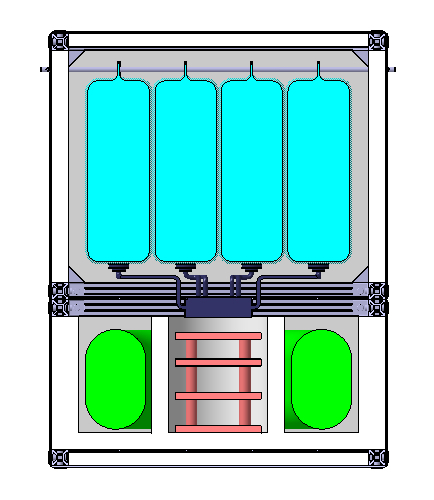
\includegraphics[width=0.7\textwidth]{4-experiment-design/img/tall_frontal.jpg}
    \caption{Cross-section of the whole experiment box.}
    \label{cut_all}
\end{figure}

The front walls, face of the experiment box exposed to the outside, will have several holes to allow the tubes providing air flow to collect clean air from the outside, see Figure \ref{front_wall_holes}.

%The top lateral walls will have four holes to allow the introduction of the circular bars used as anchor points for the sampling bags, see Figure \ref{anchor_bags}.

Bolts shall be used to attach all walls to the structure's railed bars.

%% Figure front wall holes: isometric

\begin{figure}[!ht]
    \centering
    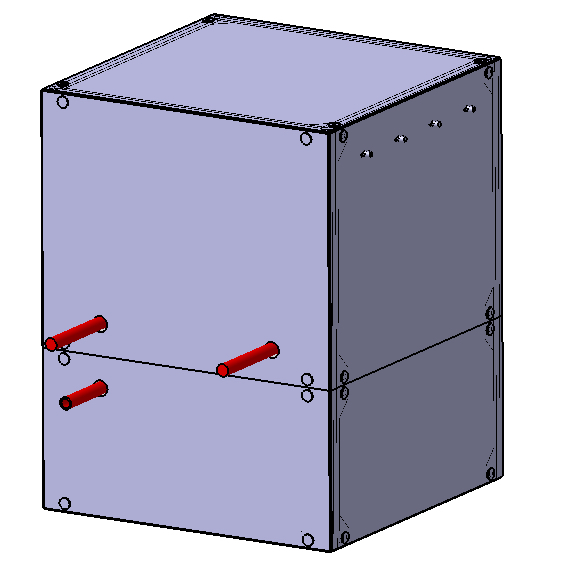
\includegraphics[width=0.7\textwidth]{4-experiment-design/img/frontal_holes.jpg}
    \caption{.}
    \label{front_wall_holes}
\end{figure}

\pagebreak
\subsubsection{Fixing Interface}

The two experiment box subsystem structures will be joined together by four anchor points. On the front and back side, two flat plates with two bolts each will interface both structures. 

This method will allow for easy and fast recovery of the CAC box. 
 

%% Figure with the two boxes attached

\pagebreak
\subsubsection{Manipulation Interface}

The two-box system will be fixed to the gondola rails by using four 90-degree angles, 2 per rail. All the anchor points will be in the AAC box since the CAC box will be already attached the it by four anchor points. The latter also ensures that the AAC box will remain properly fixed in the gondola after the CAC fast recovery. 

\smallskip
In order to access the experiment once fixed in the gondola, the walls could be removed when necessary providing access in all three directions. They can be screwed in again once the manipulation is done.


Several handles will be placed to allow an easy and safe manipulation of the experiment box in both the CAC and the AAC boxes. 


\subsubsection{Mechanical Components}

All the components used in the mechanical design can be found in Table \ref{tab:mechanical-components}. Spare elements are not included. 


\raggedbottom
\pagebreak
\subsection{Electrical Design}

\subsubsection{Block Diagram}
\label{sec:4.5.1}

The electronics design can be seen in Figure \ref{fig:electronics-block-diagram} which shows the connections, grounding, voltages, and signals. 

\begin{figure}[H]
    \begin{align*}
        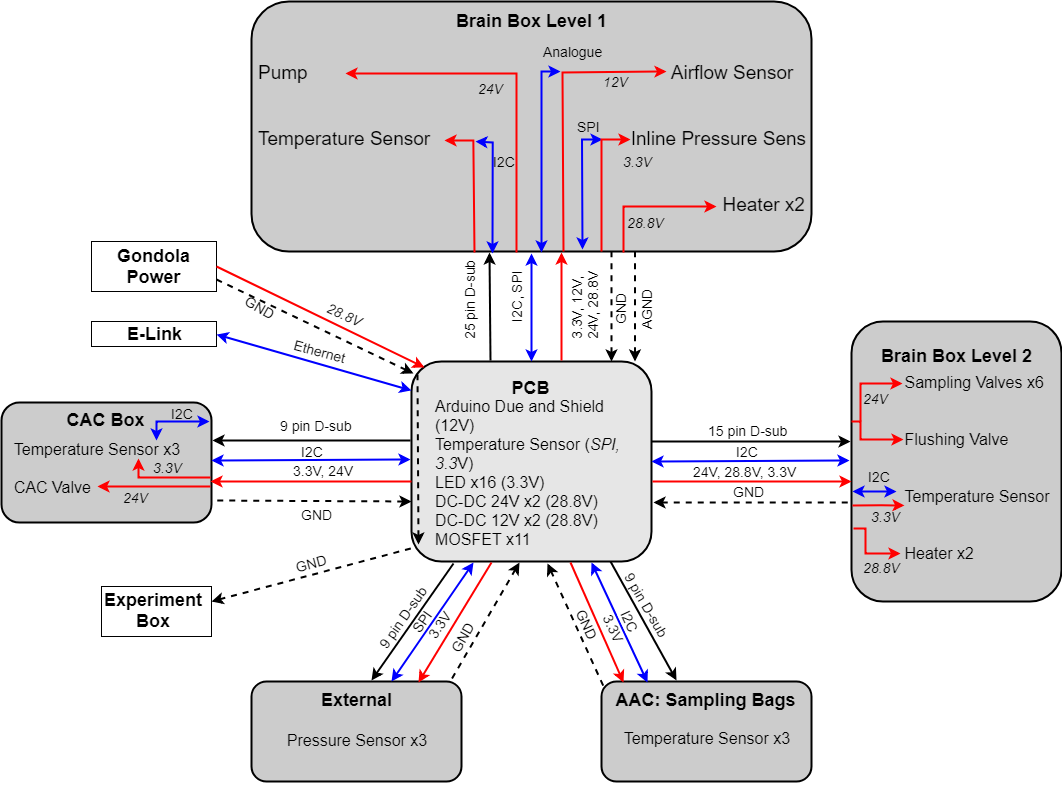
\includegraphics[width=16cm]{block-diagram-2.png}
    \end{align*}
    \caption{Block Diagram for all Electronic Components Showing the Connection, Signal and Power Connections.}\label{fig:electronics-block-diagram}
\end{figure}

Most of the electronics will be located in the Brain inside the AAC box. However, there will be six distinct areas:

\begin{enumerate}
    \item The Brain level 3, where the PCB is located with the Arudino and shield, two 24 V DC-DC, two 12 V DC-DC, one temperature sensor, 11 MOSFETs and 16 LEDs.
    \item The Brain level 2, where the valve manifolds with six sampling valves, the flushing valve, two heaters and one temperature sensor are located.
    \item The Brain level 1, where the pump, two heaters, airflow sensor, one temperature sensor and static pressure sensor are located.
    \item The AAC box, where 3 ambient temperature sensors are located.
    \item The CAC box, where the CAC valve and 3 ambient temperature sensors are located.
    \item Outside of the experiment box, where 3 ambient pressure sensors are located.
\end{enumerate}

From the PCB, on level 3, five D-sub connectors will be used to connect to the other five areas. A 25 pin connector will be used for level 1, 15 pin connector will be used for level 2 and nine pin connectors will be used for the CAC box, AAC box sampling bags area, and the external pressure sensors. In addition there will be a connection to the gondola power and gondola E-link.

All of the power distribution will take place on the PCB using two 24 V DC-DC and two 12 V DC-DC converters in parallel with a forwarding diode.  
\begin{itemize}
  \item $28.8 \, V \Longrightarrow 24 \, V $ By DC-DC converters
  \item $28.8 \, V \Longrightarrow 12 \, V$ By DC-DC converters
  \end{itemize}
The heaters will not require the voltage to be stepped down and so will be powered directly from the gondola battery.

The Arduino will control all of the sensors, valves, heaters and the pump from the PCB. Sensors will be directly connected to the Arduino. The valves, heaters and the pump will be connected via a switching circuit.

The LEDs are used as visual indicators that display whether different parts of the circuit are alive or not. They give indications on the status of the valves, pump, heaters, DC-DC converters and Arduino. 

Grounding will be following a distributed single point grounding, with all ground connections meeting at a single star point to ensure there are no floating grounds. As not all components are connected via DC-DC converters the experiment will not be isolated from the gondola power supply therefore there will be a connection between the star point and the gondola ground. The star point will be located on the main PCB board which will then be grounded to the experiment box. The grounding can be seen in Figure \ref{fig:electronics-block-diagram} where it is indicated by dashed lines labeled GND. The analog sensors that are used on level 1 in the brain use a separate grounding wire(AGND) onto the main PCB where there is a separate trace connecting to the ground pins on the Arduino board. Furthermore the upper and lower level of the main PCB board will make use of one common grounding plane.

\subsubsection{Miniature Diaphragm Air Pump}
The pump which has been selected is the 850.1.2. KNDC B, Figure \ref{fig:pumppic}, which is manufactured by KNF. One of the reasons this pump has been selected is that it has successfully been flown on a similar flight in the past where it managed to pump enough air at 25 km altitude to have 180 mL remaining at sea level \cite{LISA}. However, to ensure the pump will operate as intended, several tests will still be carried out. These tests --- 4, 5, 18, 28 and 29, can be seen in Tables \ref{tab:vacuum-test}, \ref{tab:thermal-test}, \ref{tab:pump-low-pressure-test}, \ref{tab:pump-operation-test}, and \ref{tab:pump-current-pressure-test}. The pump has already passed three of these tests and their results can be seen in Section \ref{sec:test28result} for Test 28, Section \ref{subsection:pumplowpressuretest} for Test 18 and Section \ref{sec:test29result} for Test 29.

At sea level conditions the pump was tested and found to have a flow rate of 8.0 L/min and a current draw of 250 mA. The peak current draw was recorded as 600 mA which lasts for less than one second and occurs when the pump is switched on. 

From the results of Test 18, in Section \ref{subsection:pumplowpressuretest}, the flow rate is estimated to be 3.0 L/min at the lowest pressure that will be seen in flight. This is in line with requirement D23. The results found in Test 28, in Section \ref{sec:test28result}, appear to be inline with the information given by the manufacturer, seen in Figure \ref{fig:pumpflowcur}.  The highest continuous current draw expected from the pump is 185 mA when the experiment is at 12 km altitude and is expected to decrease as we increase in altitude. While it appears the pump increases in current draw at around 6 km there is no plan to sample below 12 km therefore the highest current draw can be taken from 12 km. As the pump has a peak current of 600 mA when it switches on, the mosfet and DC-DC power have been chosen to be able to withstand this demand. 

\begin{figure}[H]
    \begin{align*}
        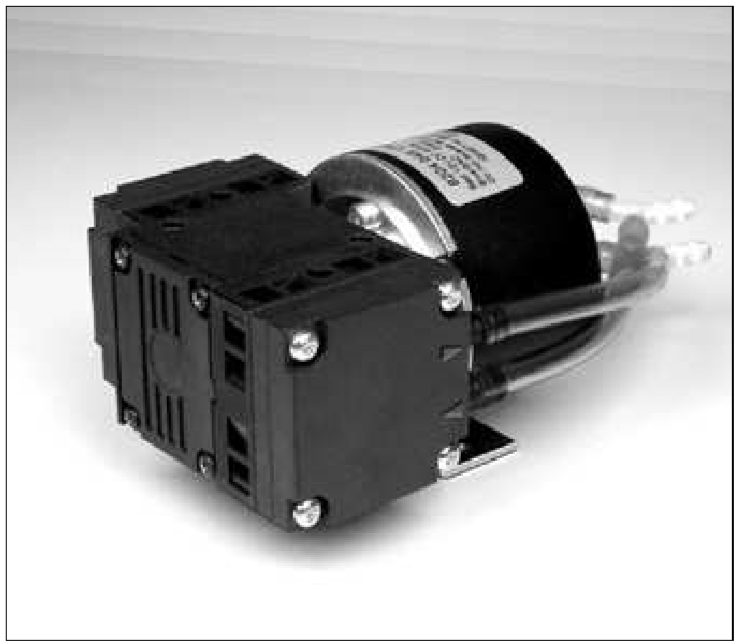
\includegraphics[width=6cm]{4-experiment-design/img/pump-850-1-2-kndc-b.png}
    \end{align*}
    \caption{KNF 850.1.2. KNDC B Miniature Diaphragm Pump.}\label{fig:pumppic}
\end{figure}


\begin{figure}[H]
    \begin{align*}
        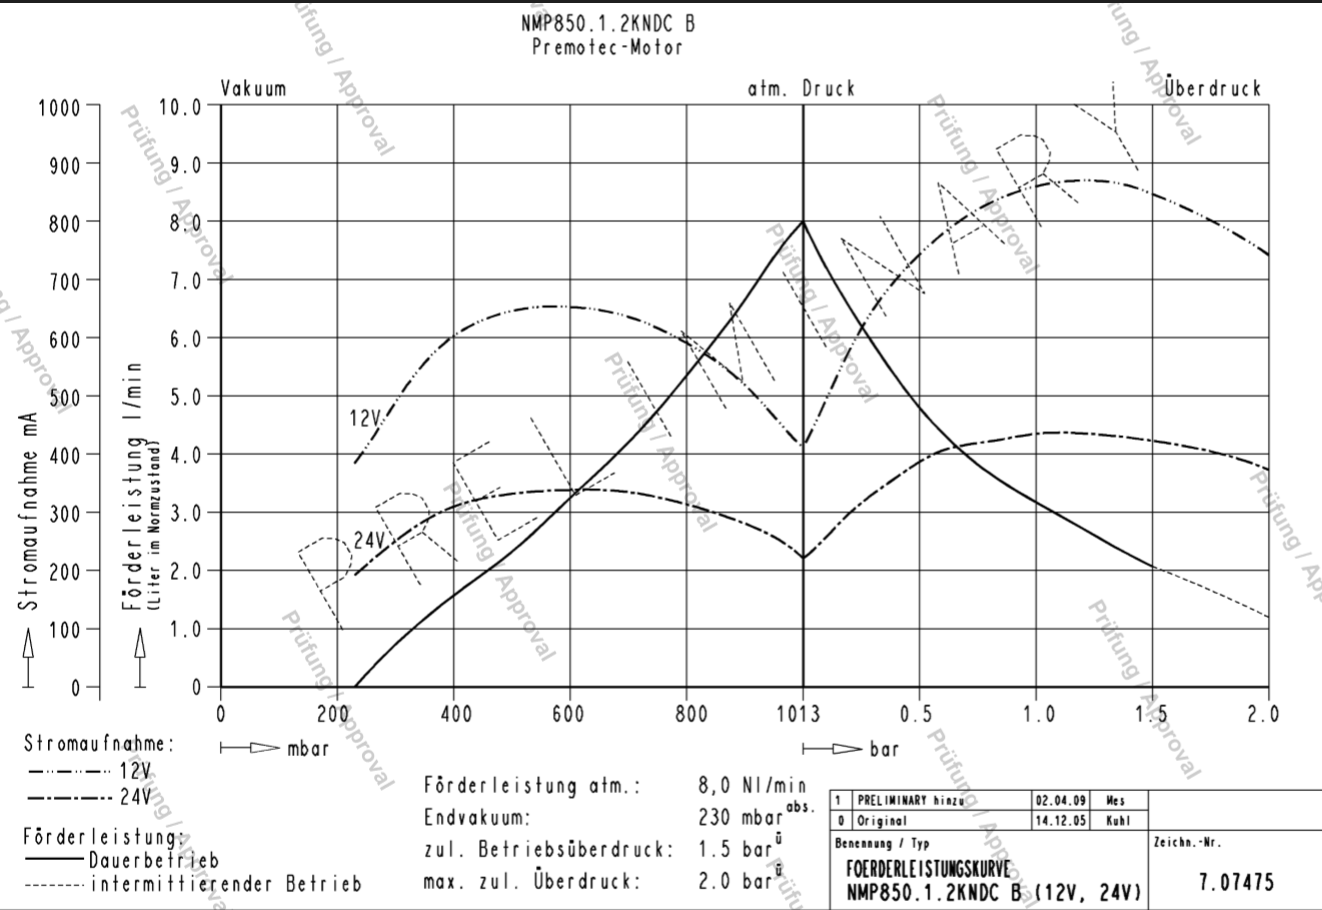
\includegraphics[width=15cm]{4-experiment-design/img/pump-flow-rate-current-graph.png}
    \end{align*}
    \caption{KNF 850.1.2. KNDC B Flow Rate and Current Draw to Pressure Graph.}\label{fig:pumpflowcur}
\end{figure}


\subsubsection{Electromagnetically Controlled Valves}
Filling the sampling bags will be controlled by solenoid valves. The solenoid valves which have been selected are model VDW23-5G-1-H-Q, seen in Figure \ref{fig:valve}, manufactured by SMC. These valves will be normally closed through out the experiment with zero power consumption and will open, when given power, to fill up the sampling bags at specific altitudes. In addition one valve will be on the CAC, in order to seal the coil at the end of the flight and another at the end of the AAC tubing, flushing valve, in order to flush the system.  The valves selected for these are model VDW22UANXB, Figure \ref{fig:valve}. The CAC valve will be opened shortly after take off and remain open the whole flight. This valve will be closed shortly before landing. The flushing valve will be opened before sampling in order to ensure the air in the tubes is from the correct altitude.

\begin{figure}[H]
    \begin{align*}
        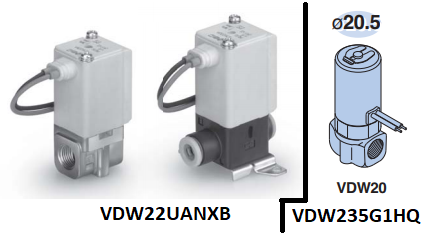
\includegraphics[width=6cm]{4-experiment-design/img/valves.png}
    \end{align*}
    \caption{SMC Solenoid Valves, VDW22UANXB on the Left, VDW23-5G-1-H-Q on the Right.}
    \label{fig:valve}
\end{figure}

The port size of the valves is 1/8" which is compatible with the gas analyzer. The coil inside can withstand temperatures from -20 to 50 °C which is suitable for flight operations at high altitudes. These valves can operate under a maximum pressure drop of 133 Pa. Valves from the same series have been flown before to the stratosphere and provided successful results \cite{LISA} however, the valves will be tested at low temperature and pressure to check they still operate as intended. These planned tests can be seen in Test 4, Table \ref{tab:vacuum-test} and Test 5, Table \ref{tab:thermal-test}.
 
\subsubsection{Switching Circuits}
The valves, pump and heaters will not be powered by the Arduino but they still need to be controlled by it. In order to allow this control a connection will be made for each component to the Arduino with a switching circuit. This switching circuit will use a eleven MOSFETs, model IRLB8748PBF, Figure \ref{fig:mosfet}, to control which components are turned on at which time.

\begin{figure}[H]
    \begin{align*}
        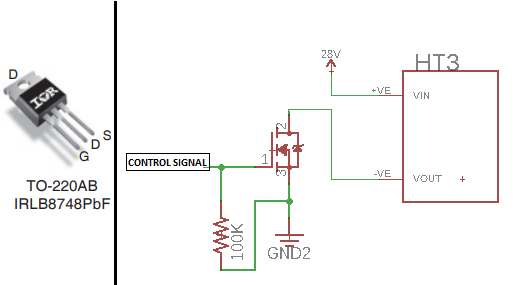
\includegraphics[width=10cm]{4-experiment-design/img/mosfet.png}
    \end{align*}
    \caption{Figure Showing an Image of the 30V,78A,75W MOSFET, Model Number IRLB8748PBF on the Left and the Schematic for the Switching Circuit for One Heater on the Right.}\label{fig:mosfet}
\end{figure}

\subsubsection{Schematic}

The schematics show all the components and how they are connected, the full schematics can be seen in Figure \ref{fig:Schematic}. There are four requirements for the the power distribution given below:

\begin{itemize}

    \item $28.8 \, V$ for the heaters.  
    
    \item $28.8 \, V \Longrightarrow 24 \, V$ for the pump and valves.
    
    \item $28.8 \, V \Longrightarrow 12 \, V$ for the airflow sensor, static pressure sensor and Arduino due.
    
    \item $3.3 \, V$ for the temperature and pressure sensors. 
    
\end{itemize}

The voltage available from gondola power is 28.8 V, therefore the heaters have been connected directly to the main power supply. For the rest of the components, two 24 V and two 12 V DC-DCs in parallel has been used to make sure if one of them fails then the other can take over. The circuitry can be seen in Figure \ref{fig:dc-dc-redun}. All the valves and the pump are then powered through the 24 V DC-DCs. To step down the voltage from 28.8 V to 12 V to power the airflow sensor, static pressure sensor and the Arduino, two 12 V DC-DCs in parallel has been used for the redundancy purposes. Finally, to power the temperature and external pressure sensors, 3.3 V is required which is supplied by the Arduino board. 

To meet the requirements of the pneumatic subsystem, a static pressure sensor has been chosen to measure the pressure inside the tubes and bags. This analogue pressure sensor operates on 12 V so can share the same power line as the airflow sensor and Arduino.


\begin{figure}[H]
    \begin{align*}
        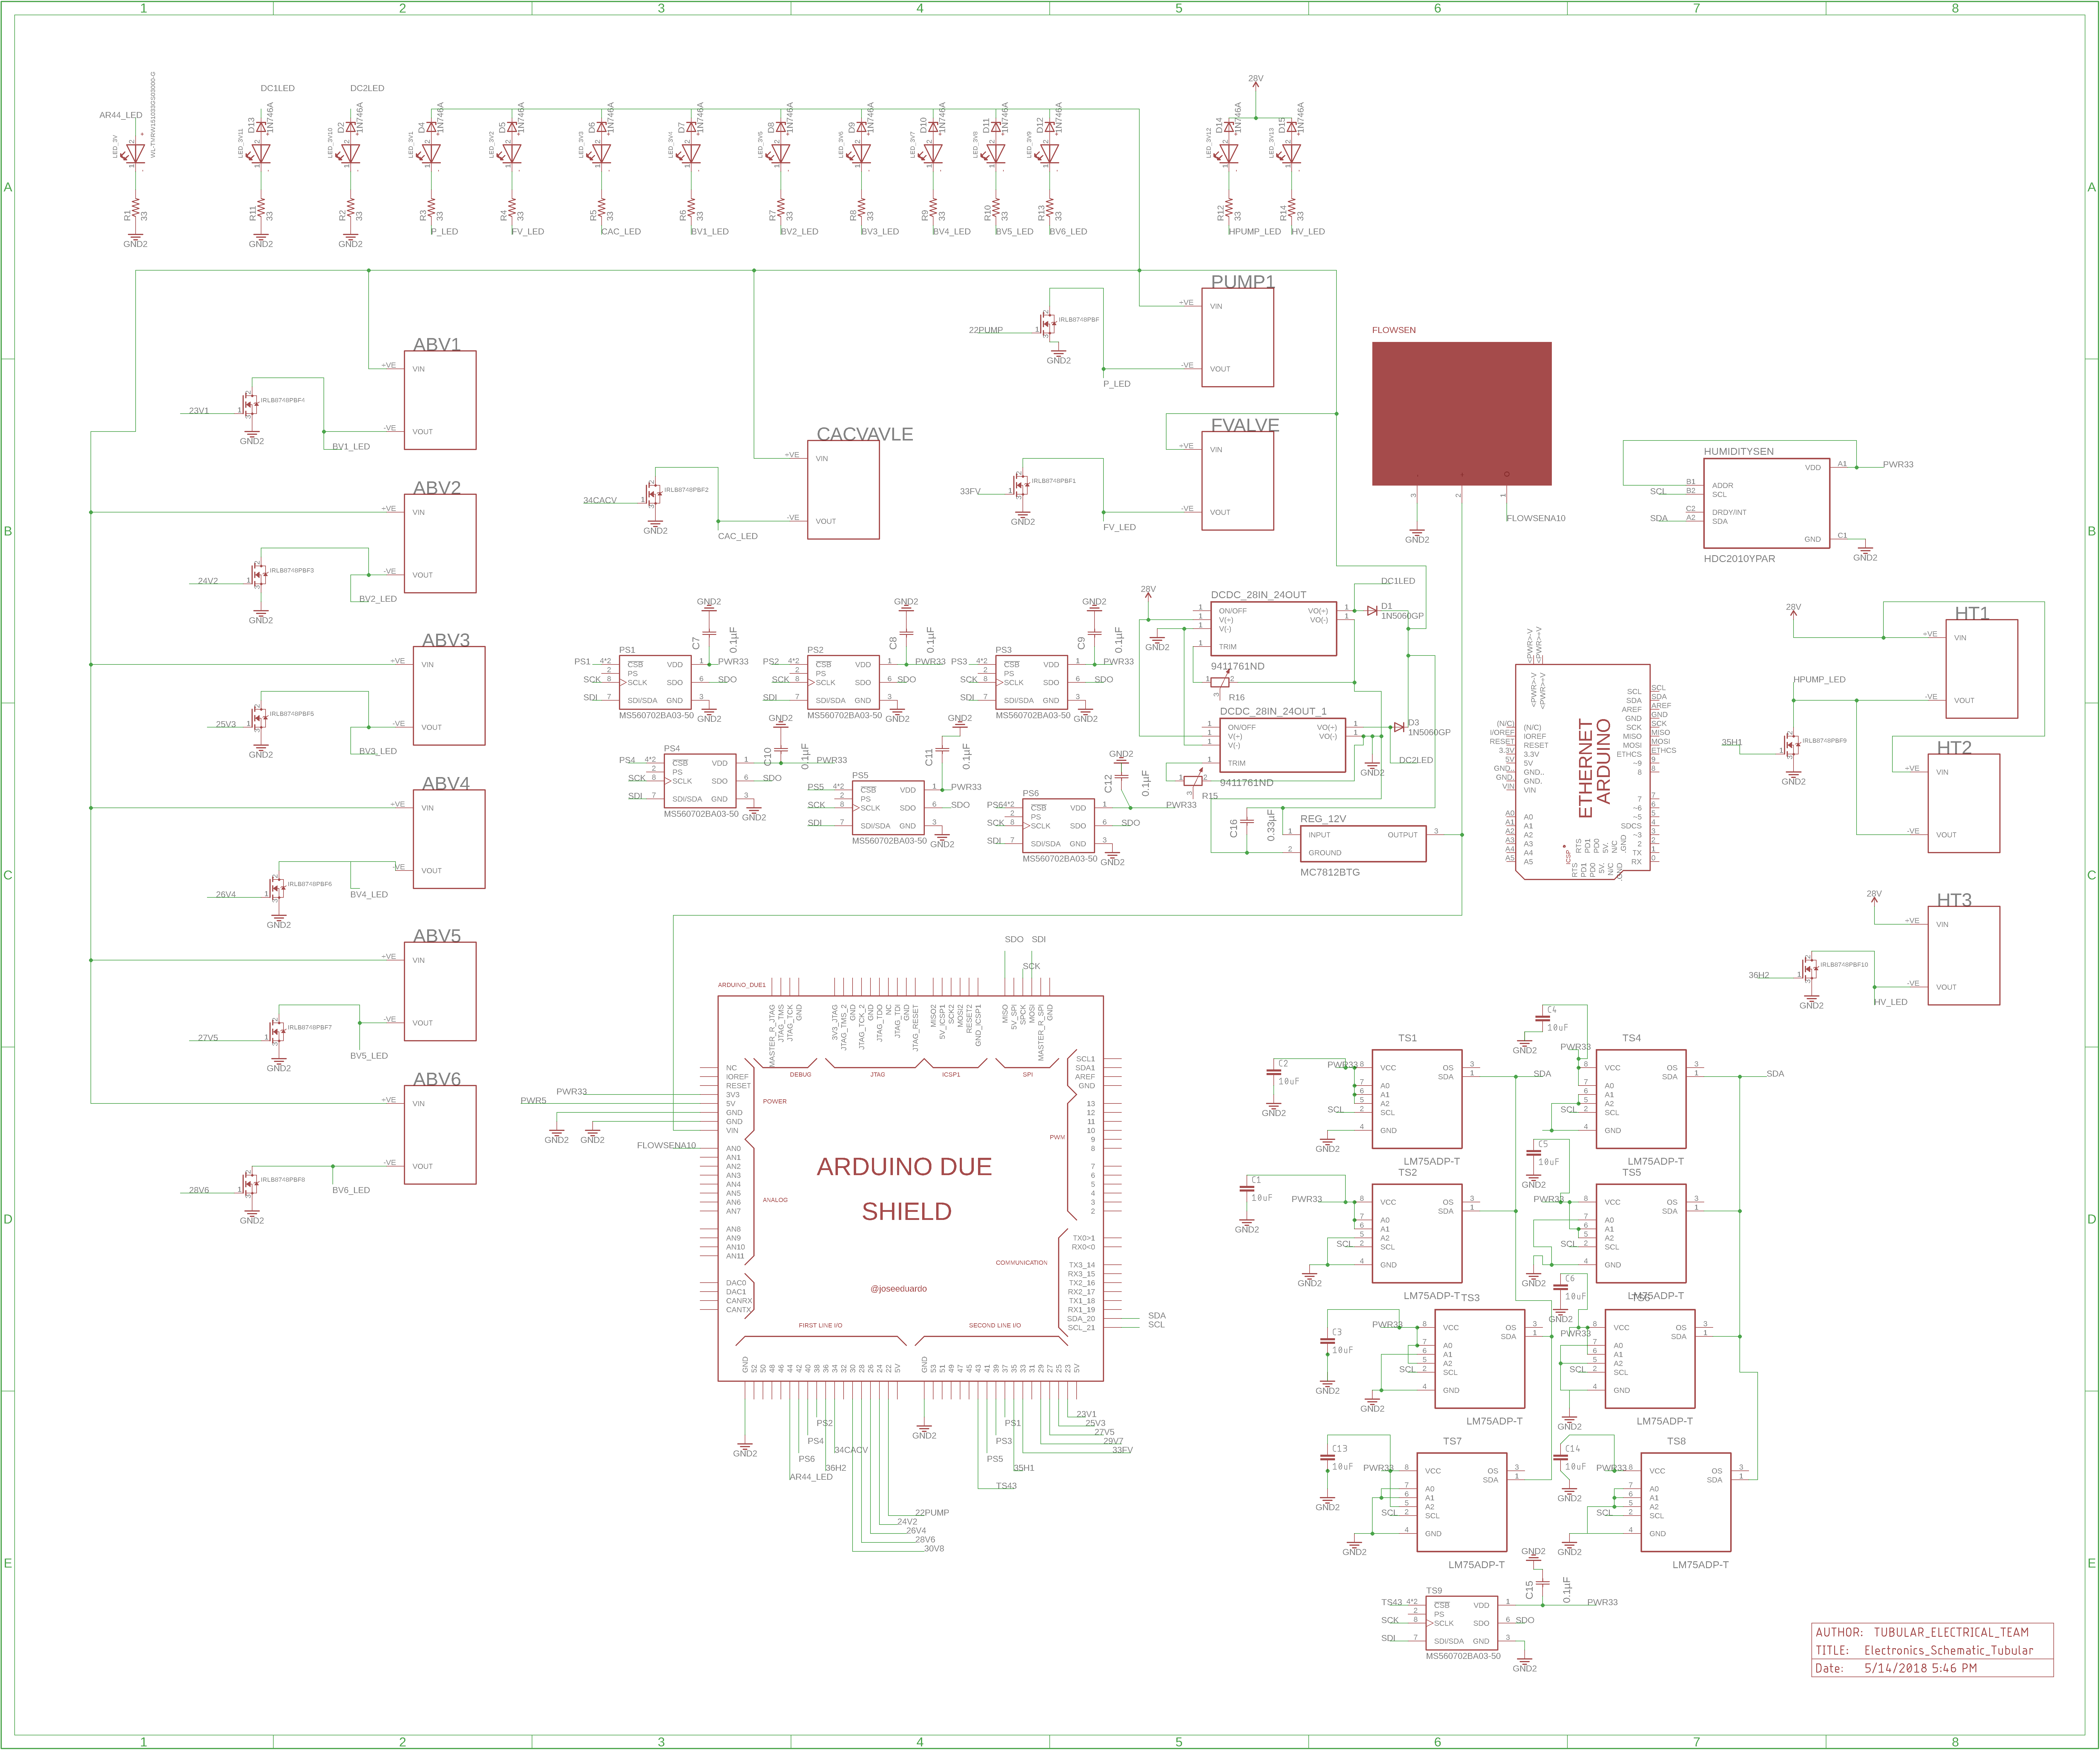
\includegraphics[width=16cm]{4-experiment-design/img/Schematics.png}
    \end{align*}
    \caption{Schematic for All of the Electronics on Board TUBULAR. This can also be Found at https://rexusbexus.github.io/tubular/img/electrical-design-schematics.png}\label{fig:Schematic}
\end{figure}

\begin{figure}[H]
    \begin{align*}
        \includegraphics[width=13cm]{4-experiment-design/img/DCDC-converter-redundancy.png}
    \end{align*}
    \caption{Schematic Showing the DC-DC Redundancy of Both 24 V  and the 12 V DC-DC Converters.}\label{fig:dc-dc-redun}
\end{figure}


\subsubsection{PCB Layout}

All electronic control circuits will be gathered on a single PCB on level 3 of the Brain. The PCB contains the Arduino due, switching circuits, indication LEDs, a temperature sensor, the power system and all necessary connectors. The connectors have been divided so that each connector's wires goes to the same level of the Brain to improve cable management. To further improve cable management the shared pins for I2C and SPI are connected to a single pin on each respective D-SUB connector and should be split up on the respective level. The PCB Layout can be seen in Figure \ref{fig:PCBLayout}.


The PCB was made using Eagle software. The traces have a width designed to fit the IPC-2221 standards\cite{IPC-2221B} with extra width added. The PCB layout can be seen in in Section \ref{sec:pcbSchematics}. On the main PCB the traces are 1.4mm wide for the nets containing components that consumes higher amounts of current and the ones with lower current requirements have a trace width of 0.3mm. On the pressure sensor PCB all traces are 0.5mm wide.




\raggedbottom
\pagebreak
\subsection{Thermal Design} \label{Thermal_section}

\subsubsection{Thermal Environment}
\begin{centering}
The experiment will experience a wide range of temperatures during the flight and it must be able to continue to operate despite these changes. As seen in Figure \ref{fig:temperature-profile} the coldest point of the flight will be between 15km and 20km where the air temperature can drop to $-80\degree$C and temperatures on the gondola have been recorded as low as $-40\degree$C during the float phase in the past \cite{BexusManual}. In addition launching from Kiruna in late October means the temperature on the ground could be as low as $-15\degree$C. As our lowest operating temperature component must be at a minimum of $0\degree$C this could mean heaters may need to be switched on while the experiment is still on the ground. 
\end{centering}


\begin{figure}[H]
    \begin{align*}
        \includegraphics[height=5cm]{4-experiment-design/img/temperature-profile.png}
    \end{align*}
    \caption{Diagram showing the temperature profile of the atmosphere \cite{jacob}}\label{fig:temperature-profile}
\end{figure}

\subsubsection{Overall Design}
\begin{centering}
To protect the components against the cold two heaters will be included. One of these will be placed close to the Arduino, which is anticipated to be able to keep the controller area warm enough, and the second will be placed close to the valves to ensure they continue to operate as expected. To control these heaters two temperature sensors will also be onboard in similar locations. If the reading from one of the temperature sensors is lower than the predefined value then the heater will turn on. 
\end{centering}


\begin{centering}
In addition to using electrical heaters the experiment will also be thermally insulated. The Styrofoam casing which will be used to protect the CAC from impact forces will also serve as insulation. It is also planned to add additional insulation around the components.  
\end{centering}

\begin{centering}
It is also important to consider heating from the sun which could raise the temperature of the experiment considerably. Sufficient insulation should be included to ensure the inside of the box stays within the operating temperature range. This will be investigated at a later date when a full CFD thermal analysis is completed.
\end{centering}
\bigskip

\pagebreak


%Added this space to help us see all of the numbers. This "Track changes" sign blocks them every time!


\begin{longtable}{|m{1cm}|m{3.5cm}|m{1.3cm}|m{1.3cm}|m{1.4cm}|m{1.3cm}|m{1.3cm}|m{1.3cm}|}
\hline
\multirow{2}{*}{\textbf{ID}} & \multirow{2}{*}{\textbf{Components}}                                 & \multicolumn{2}{l|}{\textbf{Operating (°C)}} & \multicolumn{2}{l|}{\textbf{Survivable (°C)}} & \multicolumn{2}{l|}{\textbf{Expected (°C)}} \\ \cline{3-8} &   & Min.  & Max.  & Min.  & Max.  &  Min.   &  Max.            \\ \hline
E1 & Arduino Due & -40 & 85 & -60 & 150 & -30.62 & 24.01 \\ \hline
E2 & Ethernet Shield & -40 & 85 & -65 & 150 & -30.62 & 24.01 \\ \hline
E3 & Miniature diaphragm air pump & 5 & 40 & -10 & 40 & 10 & 34.93 \\ \hline
E4 & Pressure Sensor & -40 & 85 & -40 & 125 & -19.70 & 34.93 \\ \hline
E5 & Sampling Valve (inlet and outlet 1/8"" female) & -20 & 50 & -20\footnote{If survivable temperatures were not given, operating temperatures were used as survivable limits.\label{fn:erik}} & 50\textsuperscript{\ref{fn:erik}} & -15 & 20 \\ \hline
E6 & Airflow sensor AWM43300V & -20 & 70 & -20\textsuperscript{\ref{fn:erik}} & 70\textsuperscript{\ref{fn:erik}} & -8.77 & 34.93 \\ \hline
E7 & Heater ($12.7\times 50.8 mm$) & -200 & 200 & -200\textsuperscript{\ref{fn:erik}} & 200\textsuperscript{\ref{fn:erik}} & -20 & 36 \\ \hline
E8 & Voltage Regulator & -40 & 125 & -40\textsuperscript{\ref{fn:erik}} & 125\textsuperscript{\ref{fn:erik}} & -30.62 & 34.93 \\ \hline
E9 & Temperature Sensor & -55 & 125 & -65 & 150 & -19.70 & 34.93 \\ \hline
E10 & DCDC 24 V & -40 & 85 & -55 & 125 & -19.70 & 34.93 \\ \hline
E12 & Micro SD & -25 & 85 & -200\textsuperscript{\ref{fn:erik}} & 200\textsuperscript{\ref{fn:erik}} & -19.70 & 34.93 \\ \hline
% E13 & Logic CAT5E & -20 & 75 & (-20)\textsuperscript{\ref{fn:erik}} & (75)\textsuperscript{\ref{fn:erik}} & TBD\textsuperscript{\ref{fn:ivan}} & TBD\textsuperscript{\ref{fn:ivan}} \\ \hline
% E14 & Resistors (33, 150 and 100 ohm) & -55 & 155 & (-55)\textsuperscript{\ref{fn:erik}} & (155)\textsuperscript{\ref{fn:erik}} & TBD\textsuperscript{\ref{fn:ivan}} & TBD\textsuperscript{\ref{fn:ivan}} \\ \hline
% E15 & Capacitors $(0.1 \mu$ F and $10 \mu$ F) & -30 & 85 & (-200)\textsuperscript{\ref{fn:erik}} & (200)\textsuperscript{\ref{fn:erik}} & TBD\textsuperscript{\ref{fn:ivan}} & TBD\textsuperscript{\ref{fn:ivan}} \\ \hline
E16 & Mosfet for current control & -55 & 175 & -55 & 175 & -20 & -20 \\ \hline
E17 & Diodes for DCDC converters & -65 & 175 & -65\textsuperscript{\ref{fn:erik}} & 175\textsuperscript{\ref{fn:erik}} & -19.70 & 34.93 \\ \hline
E18 & 3.3V LED & -40 & 85 & -40\textsuperscript{\ref{fn:erik}} & 85\textsuperscript{\ref{fn:erik}} & -19.70 & 24.01 \\ \hline 
E19 & 15-pin D-SUB Female connector with pins & -55 & 120 & -200\textsuperscript{\ref{fn:erik}} & 200\textsuperscript{\ref{fn:erik}} & -8.77 & 24.01 \\ \hline
E20 & 9-pin D-SUB Female connector with pins & -55 & 120  & -200\textsuperscript{\ref{fn:erik}} & 200\textsuperscript{\ref{fn:erik}} & -8.77 & 24.01 \\ \hline
E21 & 9-pin D-SUB Female connector with soldering cups & -55 & 105 & -55\textsuperscript{\ref{fn:erik}} & 105\textsuperscript{\ref{fn:erik}} & -8.77 & 24.01 \\ \hline
E22 & 9-pin D-SUB Male connector with soldering cups & -55 & 105 & -55\textsuperscript{\ref{fn:erik}} & 105\textsuperscript{\ref{fn:erik}} & -8.77 & 24.01 \\ \hline
E23 & 15-pin D-SUB Male connector with soldering cups & -55  & 105 & -55\textsuperscript{\ref{fn:erik}} & 105\textsuperscript{\ref{fn:erik}} & -8.77 & 24.01 \\ \hline
E24 & 9-pin D-SUB backing & -40 & 120 & -40\textsuperscript{\ref{fn:erik}} & 120 & -8.77 & 24.01  \\ \hline
E25 & 15-pin D-SUB backing & -40 & 120 & -40\textsuperscript{\ref{fn:erik}} & 120 & -8.77 & 24.01  \\ \hline
% E26 & Wall mounting bolts & TBD\textsuperscript{\ref{fn:ivan}} & TBD\textsuperscript{\ref{fn:ivan}} & TBD\textsuperscript{\ref{fn:ivan}} & TBD\textsuperscript{\ref{fn:ivan}} & TBD\textsuperscript{\ref{fn:ivan}} & TBD\textsuperscript{\ref{fn:ivan}} \\ \hline
E27 & D-SUB cable CAC to AAC & -40 & 85 & -55 & 125 & -40 & 40 \\ \hline
% E28 & 3.3 Zener diode & TBD\textsuperscript{\ref{fn:ivan}} & 175 & TBD\textsuperscript{\ref{fn:ivan}} & (175)\textsuperscript{\ref{fn:erik}} & TBD\textsuperscript{\ref{fn:ivan}} & TBD\textsuperscript{\ref{fn:ivan}} \\ \hline
E29 & Male connector on PCB & -40 & 85 & -40\textsuperscript{\ref{fn:erik}} & 85 & -8.77 & 24.01 \\ \hline
E30 & Female connector from wall & -40 & 85 & -40\textsuperscript{\ref{fn:erik}} & 85 & - & - \\ \hline
% E31 & Grounding contact & -55 & 125 & (-55)\textsuperscript{\ref{fn:erik}} & (125)\textsuperscript{\ref{fn:erik}} & TBD\textsuperscript{\ref{fn:ivan}} & TBD\textsuperscript{\ref{fn:ivan}} \\ \hline
E32 & Logic CAT5 E-link for inside box &-20 & 75 & -20\textsuperscript{\ref{fn:erik}} & 75\textsuperscript{\ref{fn:erik}} & -15 & 20 \\ \hline
E33 & Signal Wires & -60 & 200 & -60\textsuperscript{\ref{fn:erik}} & 200\textsuperscript{\ref{fn:erik}} & - & - \\ \hline
E34 & Flushing valve (inlet and outlet 1/8"" female) & -10 & 50 & -10\textsuperscript{\ref{fn:erik}} & 50\textsuperscript{\ref{fn:erik}} & -7.36 & 42.53 \\ \hline
E35 & Valves manifold (outlet 1/8"" female) & -10 & 50 & -10\textsuperscript{\ref{fn:erik}} & 50\textsuperscript{\ref{fn:erik}} & -6.77 & 40.504 \\ \hline
E36 & Power wire black & -60 & 200 & -60\textsuperscript{\ref{fn:erik}} & 200\textsuperscript{\ref{fn:erik}} & - & - \\ \hline
% E37 & Electrical Tape for marking wires (White) & -10 & 90 & (-10)\textsuperscript{\ref{fn:erik}} & (90)\textsuperscript{\ref{fn:erik}} & TBD\textsuperscript{\ref{fn:ivan}} & TBD\textsuperscript{\ref{fn:ivan}} \\ \hline
% E38 & Electrical Tape for marking wires (Black) & -10 & 90 & (-10)\textsuperscript{\ref{fn:erik}} & (90)\textsuperscript{\ref{fn:erik}} & TBD\textsuperscript{\ref{fn:ivan}} & TBD\textsuperscript{\ref{fn:ivan}} \\ \hline
% E39 & Electrical Tape for marking wires (Green) & -10 & 90 & (-10)\textsuperscript{\ref{fn:erik}} & (90)\textsuperscript{\ref{fn:erik}} & TBD\textsuperscript{\ref{fn:ivan}} & TBD\textsuperscript{\ref{fn:ivan}} \\ \hline
% E40 & Electrical Tape for marking wires (Violet) & -10 & 90 & (-10)\textsuperscript{\ref{fn:erik}} & (90)\textsuperscript{\ref{fn:erik}} & TBD\textsuperscript{\ref{fn:ivan}} & TBD\textsuperscript{\ref{fn:ivan}} \\ \hline
% E41 & Electrical Tape for marking wires (Gray) & -10 & 90 & (-10)\textsuperscript{\ref{fn:erik}} & (90)\textsuperscript{\ref{fn:erik}} & TBD\textsuperscript{\ref{fn:ivan}} & TBD\textsuperscript{\ref{fn:ivan}} \\ \hline
% E42 & Electrical Tape for marking wires (Brown) & -10 & 90 & (-10)\textsuperscript{\ref{fn:erik}} & (90)\textsuperscript{\ref{fn:erik}} & TBD\textsuperscript{\ref{fn:ivan}} & TBD\textsuperscript{\ref{fn:ivan}} \\ \hline
% E43 & Electrical Tape for marking wires (Blue) & -10 & 90 & (-10)\textsuperscript{\ref{fn:erik}} & (90)\textsuperscript{\ref{fn:erik}} & TBD\textsuperscript{\ref{fn:ivan}} & TBD\textsuperscript{\ref{fn:ivan}} \\ \hline
% E44 & Heat shrinking tube 2.5 x 1mm & -55 & 125 & (-55)\textsuperscript{\ref{fn:erik}} & (125)\textsuperscript{\ref{fn:erik}} & TBD\textsuperscript{\ref{fn:ivan}} & TBD\textsuperscript{\ref{fn:ivan}} \\ \hline
E45 & 25-pin D-SUB female connector with pins & -10 & 90 & -10\textsuperscript{\ref{fn:erik}} & 90\textsuperscript{\ref{fn:erik}} & -8.77 & 24.01 \\ \hline
E46 & 25-pin D-SUB male connector with soldering cups & -10 & 90 & -10\textsuperscript{\ref{fn:erik}} & 90\textsuperscript{\ref{fn:erik}} & -8.77 & 24.01 \\ \hline
E47 & 25-pin D-SUB backing & -10 & 90 & -10\textsuperscript{\ref{fn:erik}} & 90\textsuperscript{\ref{fn:erik}} & -8.77 & 24.01 \\ \hline
E48 & Power wire red & -60 & 200 & -60\textsuperscript{\ref{fn:erik}} & 200
\textsuperscript{\ref{fn:erik}} & - & -  \\ \hline
% E49 & Potentiometer 1k ohm & -55 & 125 & (-55)\textsuperscript{\ref{fn:erik}} & (120)\textsuperscript{\ref{fn:erik}} & TBD\textsuperscript{\ref{fn:ivan}} & TBD\textsuperscript{\ref{fn:ivan}} \\ \hline
E50 & 6-pin male & -55 & 105 & -55\textsuperscript{\ref{fn:erik}} & 105\textsuperscript{\ref{fn:erik}} & -8.77 & 24.01  \\ \hline
E51 & 8-pin male single row header& -40 & 105 & -40\textsuperscript{\ref{fn:erik}} & 105\textsuperscript{\ref{fn:erik}} & -8.77 & 24.01  \\ \hline
E52 & 10-pin male single row header & -55 & 105 & -55\textsuperscript{\ref{fn:erik}} & 105\textsuperscript{\ref{fn:erik}} & -8.77 & 24.01  \\ \hline
E53 & 36-pin male double row header & -40 & 105 & -40 & 125 & -8.77 & 24.01  \\ \hline
E54 & 12 V DC/DC converter & -40 & 85 & -55 & 125 & -8.77 & 24.01  \\ \hline
E56 & Pressure Sensor & -40 & 120 & -40\textsuperscript{\ref{fn:erik}} & 120\textsuperscript{\ref{fn:erik}} &  -8.77 & 34.93 \\ \hline


\caption{Table of Component Temperature Ranges.}
\label{tab:thermal-table}
\end{longtable}
\raggedbottom










\raggedbottom

\subsubsection{Internal Temperature}

As the current experiment model stands, an enclosed partition has been reserved in the lower front-right corner of the AAC section of the TUBULAR experiment. This partition will house all of the electronic components not required to be situated in specified locations throughout the experiment setting, such as some of the sensors. 

Inside this partition will be three separate insulated boxes. The first of these is the Electronics box which will occupy a space measuring 20 cm in length, 10 cm in width, and 20 cm in height, and will be insulated from inside to outside with polyethylene, polystyrene, and finally aluminum. The infrastructure within this enclosure shall be such that the electronics are fitted together to in turn be bound within another box of insulated material (likely made from PVC). 

Above the electronics box will be the second internal box, the pump box, where the pump will be situated and the third internal box, the valve centre, where the valves will be situated. The valves will be routed together by several tubes to form a compact structure aiding the thermal control over this area. 

One heater will be included in the electronics box with its main priority being keeping the Arduino Due board within operational temperatures whilst delivering the remaining heat to peripheral electronics. The other heater will be fitted between the pump and the entrances to the valve center and will keep its lateral neighbors within their respective operational temperature ranges.

The pump has the most critical temperature range as it is the only component that cannot operate below freezing temperatures. It's data sheet states it must always be no colder than $5\degree$C, or the EPDM diaphragm may not be able to expand and contract sufficiently to maintain the desired airflow of 8L/min. However as this pump has been used successfully on flights before, \cite{LISA}, tests will be conducted on the pump to find its true performance at lower temperatures. The valves are also crucial to the experiment's function, as they enable each and every sampling bag onboard to be used. For this reason, while the valves can operate down to $-43\degree$C, it is desirable to be keep them above this limit whenever in use.

Given the thermal conductivity of EPDM ($0.2 W/(m.K)$), the pump's diaphragm experiences a minimal temperature drop across itself when one side is subject to the heater's temperature while the other end of the pump is leveled with the ambient temperature. Through calculation it was found that at an ambient temperature of $-50\degree$C and a heater temperature at $10\degree$C, the center of the pump, the far end of the diaphragm, measured $9.35\degree$C. Reassessing the equation yielded the most energy-conserving temperature that would keep the pump's diaphragm above the minimum requirement to be $7\degree$C. This held whether the temperature was as it could be on ground level ($-10\degree$C), or in floating phase ($-50\degree$C).

Symbols used are the following:

\begin{itemize}
    \item $T_{inlet}$ &= Temperature at the pump inlet face
    \item $T_{heated}$ &= Temperature at the pump's diaphragm face (directly heated)
    \item $L_{inlet}$ &= Length of the pump inlet valve(s)
    \item $L_{phragm}$ &= Length of the pump's diaphragm
    \item $k_{PPS}$ &= Thermal conductivity of the pump's inlet valve(s) made of PPS
    \item $k_{EPDM}$ &= Thermal conductivity of the pump's diaphragm made of EPDM
    \item $k_{air}$ &= Thermal conductivity of the air entering the pump
    \item $k_{phragm}$ &=  Averaged thermal conductivity of the pump's diaphragm (Assumed 4 parts air to 1 part EPDM)
    \item $T_{med}$ &= Temperature halfway across the pump (start of the diaphragm)
\end{itemize}




 \begin{align*}
    T_{inlet} &= 263 K\\
    T_{heated} &= 283 K\\
    L_{inlet} &= 0.038 m\\
    L_{phragm} &= 0.038 m\\
    k_{PPS} &= 2\frac{W}{m\cdot K}\\
    k_{EPDM} &= 0.2\frac{W}{m\cdot K}\\
    k_{air} &= 0.024\frac{W}{m\cdot K}\\
    k_{phragm} &=  \frac{(k_{EPDM}+4\cdotk_{air})}{5} = 0.06\frac{W}{m\cdotK}\\
    T_{med} &= \frac{( k_{phragm}\cdot   L_{inlet}\cdot T_{inlet}) + (k_{PPS}\cdot L_{phragm}\cdot T_{heated}) }{ (k_{phragm}\cdot L_{inlet}) + (k_{PPS} \cdot L_{phragm})} \\
    T_{med} &= \frac{ (0.06\cdot  0.038\cdot 263) + (2\cdot 0.038\cdot 283)}{(0.06\cdot 0.038) + (2\cdot 0.038)} \\
    T_{med} &= 282.35 K \longrightarrow 9.35\degree C
 \end{align*}

Reworking the equation to fit the inlet face at the true ambient temperature of -50$\degree$C and the reduced heater temperature of 7$\degree$C gives the following:

% nice :) Also remove the * and it will number the equations. Also also to start a new line just write \\ at the end and it will make the next thing appear on a new line. Also also also using &= aligns all the equals signs and makes it look nice :D I leave these tips here so delete when you don't need them :)


 \begin{align*}
     T_{inlet} &= 223 K\\
    T_{heated} &= 280 K\\
    T_{med} &= \frac{ (k_{phragm}\cdot L_{inlet}\cdot T_{inlet}) + (k_{PPS}\cdot L_{phragm}\cdot T_{heated}) }{ (k_{phragm}\cdot L_{inlet}) + (k_{PPS}\cdot L_{phragm})}\\
    T_{med} &= \frac{ (0.06\cdot 0.038\cdot 223) + (2\cdot 0.038\cdot 280)}{(0.06\cdot 0.038) + (2\cdot 0.038)}\\
    T_{med} &= 278.28 K \longrightarrow 5.28\degree C
 \end{align*}

\newpage
\subsubsection{Box Analysis}

For the box temperature to be properly estimated, the other two divisions within the component enclosure need to be taken into account. The manifold comprising the valve center is made of a compound of nylon (assumed to be nylon-6) and kynar. It has also been assumed they are used equally in mass and distribution at this stage of the thermal estimation.

Symbols used are the following:

\begin{itemize}
    \item $T_{outlet}$ &= Temperature at the manifold's outlet(s)
    \item $T_{heated}$ &= Temperature of the pump at its diaphragm face
    \item $L_{outhalf}$ &= Length of the outer half of the manifold
    \item $L_{inhalf}$ &= Length of the inner half of the manifold
    \item $k_{Nylon-6}$ &= Thermal conductivity of Nylon-6
    \item $k_{Kynar}$ &= Thermal conductivity of Kynar
    \item $k_{manifold}$ &= Averaged thermal conductivity of manifold
\end{itemize}


 \begin{align*}
    T_{outlet} &= 263 K\\
    T_{heated} &= 283 K\\
    L_{outhalf}& = 0.038 m\\
    L_{inhalf} &= 0.038 m\\
    k_{Nylon-6} &= 0.24\frac{W}{m\cdot K}\\
    k_{Kynar} &= 0.162\frac{W}{m\cdot K}\\
    k_{manifold} &=  \frac{k_{Nylon-6}+k_{Kynar}}{2} = 0.201\frac{W}{m\cdot K}\\
    T_{med} &= \frac{ (k_{manifold}\cdot L_{inhalf}\cdot T_{heated}) + (k_{manifold}\cdot L_{outhalf}\cdot T_{outlet}) }{ (k_{manifold}\cdot L_{inhalf}) + (k_{manifold}\cdot L_{outhalf})}\\
    T_{med} &= \frac{ (0.201\cdot 0.040\cdot 223) + (0.201\cdot 0.040\cdot 280)}{(0.201\cdot 0.040) + (0.201\cdot 0.040)}\\ 
    T_{med} &= 251.59 K \longrightarrow -21.41\degree C
 \end{align*}
 
 
\newpage
Below, in Figure \ref{fig:enclosurebox} is a theoretical general arrangement of the components within the enclosure, seen from the front of the experiment inward.
 
 \begin{figure}[H]
    \begin{align*}
        \includegraphics[height=8cm]{4-experiment-design/img/bexus-thermal-first.png}
    \end{align*}
    \caption{Diagram showing a general layout of the AAC components}
    \label{fig:enclosurebox}
\end{figure}
 
 A rough estimation of temperature gradients can thus be shown in Figure \ref{fig:boxanalysis}:
 
 \begin{figure}[H]
    \begin{align*}
        \includegraphics[height=8cm]{4-experiment-design/img/bexus-thermal-second.png}
    \end{align*}
    \caption{Diagram of the previous layout now showing temperature contours}
    \label{fig:boxanalysis}
\end{figure}


\pagebreak
\subsection{Power Design}

\subsubsection{Power System Requirements}
\begin{centering}
The Gondola provides 28.8 V or 13 Ah battery with a recommended maximum current draw of 1.8A \cite{BexusManual}. The experiment must run on external power from 4 hours before launch during the countdown phase and for the entire flight duration, lasting approximately 4 hours. As a factor of safety the experiment should be able to run for an additional 2 hours. Therefore in total the experiment must be able to run for 10 hours on external power.
\end{centering}

\begin{longtable}{|m{0.03\textwidth}| m{0.3\textwidth} |m{0.14\textwidth} |m{0.16\textwidth}|m{0.13\textwidth}| m{0.14\textwidth} |}
\hline
\textbf{ID}             & \textbf{Component}                                                   & \textbf{Voltage {[}V{]}} & \textbf{Current {[}mA{]}} & \textbf{Power {[}W{]}} & \textbf{Total {[}Wh{]}} \\ \hline
1                       & Arduino Due                                       & 12                                          & 30                                           & 0.36                                      & 36                                         \\ \hline
2                       & \hl{BTC Series PMDC Iron Core Brush Miniature Diaphragm Pump H084-11} \st{Micro Air Pump CMP30-3PW}                          & 24                                          & \hl{180} \st{300}                                          &\hl{4.32} \st{7.2}                                       & \hl{4.32} \st{7.2}                                        \\ \hline
3                       & Barometric Pressure Sensor MS5607-02BA03          & 3.3                                         & 1.4                                          & 0.00462                                   & 0.1                                        \\ \hline
4                       & Electromagnetically controlled valve              & 24                                          & 458                                          & 11                                        & 75                                         \\ \hline
5                       & Airflow sensor AWM40000 Series                    & 10                                          & 6                                            & 0.060                                     & 0.6                                        \\ \hline
6                       & Polyimide Thermofoil Heaters HK5161R78.4L12       & 28                                          & 357                                          & 10                                        & 100                                        \\ \hline
7                       & Polyimide Thermofoil Heaters HK5160R157L12        & 28                                          & 179                                          & 5                                         & 50                                         \\ \hline
8                       & Temperature sensor VSSOP-8, LM70, LM70CIMM-5/NOPB & 5.5                                         & 0.49                                         & 0.002695                                  & 0.054                                      \\ \hline
9                       & DC-DC step converter                              & 28                                          & 500 (output)                                 & 0.09                                      & 0.9                                        \\ \hline
10                      & HDC2010 Low Power Humidity Digital Sensors        & 3.3                                         & 0.0005                                       & 1.65$\times10^{-6}$                              & 16.5$\times10^{-6}$                               \\ \hline
\multicolumn{1}{|c|}{-} & \textbf{Total}                                  & \multicolumn{1}{c|}{-}                      & \multicolumn{1}{c|}{\hl{1671} \st{1791}}                    & \multicolumn{1}{c|}{\hl{41.42} \st{44.3}}                 & \hl{267} \st{270}                                        \\ \hline
\multicolumn{1}{|c|}{-} & \textbf{Available from gondola}                 & \multicolumn{1}{c|}{-}                      & \multicolumn{1}{c|}{-}                       & \multicolumn{1}{c|}{-}                    & 374                                        \\ \hline

\caption{Power Design Table}
\label{tab:power-design-table}
\end{longtable}
\raggedbottom

%   $16.5\times10^{blah}$

\subsubsection{Power System Control and Regulation}
The power on board will be split using three DC-DC converters and one linear regulator. The pump and valves both have a high peak current. Therefore it was decided to use two DC-DC converters to step down from 28.8V to 24V giving the pump its own dedicated DC-DC converter. This is as the pump and valves both have a high rush in current. The Arduino will also have its own DC-DC converter stepping the voltage down from 28.8V to 12V. The linear regulator will be placed after the 24V DC-DC converter to act as redundancy for the 12V DC-DC converter. If for some reason the 12V DC-DC converter should fail it will take over ensuring that power to the Arduino is not lost. To ensure takeover does not occur when the 12V DC-DC converter is operating a diode shall be placed along the connection. It is thought using three DC-DC converters will provide the best compromise between efficiency, cost and heating.

\raggedbottom

\pagebreak
\subsection{Software Design}
\subsubsection{Purpose}
The purpose of the software was to automate control of the valves so that they will be opened/closed at the target altitude. Moreover, the software stored housekeeping data from sensors, pump, and valves states to the on-board memory storage device. Logging sensor data was necessary in order to determine a vertical profile of the analyzed samples:

\begin{quote}
In order to determine the vertical profiles of CO$_2$, CH$_4$, and CO from the analysis of sampled air, measurements of several atmospheric parameters were needed [...]. The two most important parameters were the ambient pressure and the mean coil temperature. These parameters were be recorded by the AirCore-HR (High Resolution) electronic data package. Mean coil temperature was obtained by taking the mean of three temperatures recorded by independent probes located at different positions along the AirCore-HR.\cite{Membrive}
\end{quote}

Both the ambient pressure and the sampling container temperature were also essential for AAC sampling bags. The temperature data was collected by the sensors near the sampling bags.

The software shall also transmit data to the ground so that the team can monitor the conditions of the experiment in real time. Telecommand was also needed to overwrite pre-programmed sampling scheduled in case of automation failure or to mitigate unexpected changes in the flight path and reached altitudes. It was used to test the system, especially valves and heaters.\par

\subsubsection{Design} \label{sec:4.8.2}
\begin{enumerate}[label=(\alph*)]
\item{Process Overview}\\
The software which ran on the Arduino read from the sensors through the analog, I2C, and SPI interfaces. The sensors provided temperature, pressure and airflow data. The acquired data was time-stamped and stored in the on-board SD card and transmitted via the E-Link System to the ground station. Then according to the pressure/altitude, the software controlled the valves which allowed the air to be pumped inside the bags. Figure \ref{processOverview} visually explain the process flow.

\begin{figure}[H]
    \centering
    \includegraphics[width=0.85\textwidth]{4-experiment-design/img/Process-overview-V0-3.png}
    \caption{The Process Overview of the Experiment.}
    \label{processOverview}
\end{figure}

\item{General and Safety related concepts}\\
The watchdog timer, which was an electronic countdown timer that causes an interrupt when it reaches 0, was used to avoid failure because of a possible freezing problem in the software. During normal operations, the software set flags when done with their task. When all the flags had been set the watchdog got reset. If any task fails to set the their flag before the watchdog elapses, the system resets. Telecommand was also be used as backup in case the automation fails or otherwise become unresponsive. Telemetry was utilized to transmit housekeeping data and the state of the valves to get confirmation of operation. Rigorous testing was performed during the development of the project and before the launch phase to insure that that the software was capable to control the experiment.
\item{Interfaces}\\
Table \ref{tab:comIntpro} demonstrates how the components interacted with the onboard computer (OBC). Components that used SPI, shared MISO, MOSI, and CLK pins on the Arduino board. Each of them was also connected to general pins input output (GPIO) for slave select. Furthermore, components using I2C protocol, shared Serial Data pin (SDA) and Serial Clock pin (SCL).

\begin{table}[H]
\centering
\begin{tabular}{lll}
Components interacting & Communication protocol & Interface                 \\ \hline
Pressure Sensors-OBC   & SPI                    & Arduino SPI and Digital Pins \\
Temperature sensors-OBC        & I2C                    & Arduino I2C \\
Airflow sensor-OBC     & I2C                    & Arduino I2C \\
Heaters-OBC            & Digital                & GPIO pins \\
Air pump-OBC           & Digital                & GPIO pins \\
Valve-OBC              & Digital                & GPIO pins                 \\
OBC-microSD Storage    & SPI                    & Arduino Ethernet shield   \\
OBC - E-Link           & Ethernet               & Ethernet port            
\end{tabular}%Tabular dude
\caption{Communication and interface protocols}
\label{tab:comIntpro}
\end{table}

Every transmission to/from the ground utilized the E-link connection. The data packet which was used was an Ethernet Packet with a header containing the address of destination, followed by the data, and at the end there was a frame check sequence (FCS). The up-linked data packet had the same structure, with header followed by commands and ended with FCS.\\
\\
The protocol that had been chosen was UDP for telemetry and TCP for telecommand. The UDP was used to prevent software getting stuck waiting for handshake from the ground if the connection was temporarily lost.\\
\\
The telecommand contained the following services:
\begin{itemize}
    \item Changing instrument modes
    \item Manually control valves, pump, and heaters
    \item Change sampling schedule
\end{itemize}

Furthermore, telemetry contained the services below:
\begin{itemize}
    \item Data from temperature, pressure and airflow sensor
    \item Current instrument modes
    \item Instrument housekeeping data (valve, pump, and heater states)
\end{itemize}
\item{Data Acquisition and Storage}\\
Data was stored on the SD memory card on the Arduino Ethernet Shield using the FAT16 and FAT32 file systems. To minimize data loss in the event of a reset, the same file was written only in a set amount of time before closing it and opened a new file. It was estimated that for the entire flight, all the sensors produced less than $5$ MB of data. The sampling rate was fixed at 1 sampling per second.\\
\\
The data was collected and presented as a matrix, where the first column was the time frame, the following columns were the sensors data. After the sensors data, there was also housekeeping data, that kept track of the valves, and heaters states. However, the size of the housekeeping data was not expected to surpass 20 bits per sampling.\\
\\
Data was continuously down-linked two times per second and the total telemetry size was less than $4$ MB for 10 hours of flight. The telecommand size was on the other hand varied based on how many subcommands were sent each time. If all of the subcommands were enabled, the total size was 128 bytes. Considering the telecommand was not sent more than once per second, the telecommand data rate was 126 bytes/sec.
\item{Process Flow}\\
The process flow can be explained with the mode diagram in Figure \ref{fig:modediag}. The software started with Standby Mode, in which the software got samples from all sensors. The on-board memory card contained the default sampling schedule parameters (when the sampling will start and stop), which was read by the software during initialization of the OBS. This allowed users to change the sampling schedule without changing the internal code. When the software received negative increment of pressure changes, it changed to Normal - Ascent mode, where the software triggered emptying of the CAC's coiled tube by opening the valves. Then, at certain altitudes, air sampling was conducted during Ascent Phase. During Float Phase, no sampling was conducted. The software went to Normal - Descent mode when it detected the increment of pressure was considerably big at which point the software sampled the air by opening the valves for each bag in their designated altitude. Considering that the gondola might not have smooth ascent/descent, the mode changes only happened if the changes exceeded a certain threshold. After analysis and testing, $\SI{-20}{h\pascal}$ and $\SI{20}{h\pascal}$ were considered as the threshold. The experiment went to SAFE mode approximately \SI{1200}{\meter} before the landing, and triggered all the valves to be closed. The manual mode was entered with a telecommand and left with another one. If no telecommand was received by the OBC within a certain amount of time it left manual mode and entered into standby mode.

\begin{figure}[H]
    \begin{align*}
        \includegraphics[scale=0.55]{4-experiment-design/img/state-diagram-V1-3.png}
    \end{align*}
    \caption{Process Diagram for the Modes.}\label{fig:modediag}
\end{figure}

In the sampling algorithm, it was necessary to keep track of the time because the bag could not be filled fully (it might burst). A simple library was used to keep track of the time from the start of the experiment.\par 

\item{Modularization and Pseudo Code}\\
\begin{figure}[H]
    \begin{align*}
        \includegraphics[width=1\linewidth]{4-experiment-design/img/sw_design_v1-8.png}
    \end{align*}
    \caption{Onboard Software Design Tree.}\label{fig:obtree}
\end{figure}

The software design was produced by using object oriented approach. The functionality of the experiment was divided into several objects and their children. The design tree is shown in Figure \ref{fig:obtree}.\\
\\
The Telemetry object was responsible to format the sensor/housekeeping data, and to transmit it. MODE was responsible for controlling the five modes of software. INIT initialized the necessary software. COMMANDS read the telecommands and executed their commands. The AIR SAMPLING CONTROL object had the four children objects. The first child was responsible for controlling the pump. The second child contained the parameters for the valves and pump. The third child read the data from the sensors, a fourth child was responsible for manipulating the valves.\\
\\
The SENSOR object had two children objects. One for sampling the sensors and another for recording and storing the housekeeping data. The HEATER object had three children objects. One for reading the temperature sensor data, another for deciding if the heaters should be turn on/off. And the third child for turning it on/off.\\ 
\\
The MONITOR object utilized a watchdog timer that caused an interrupt when it reaches 0. The watchdog did not get fed directly from by the end of the different tasks. Instead the tasks set a flag, if all the flags were set the watchdog got reset and the countdown started from the beginning. If the watchdog timed out before all the flags were set the monitor object reset the board.\\
\\
Each of the objects interacted with each others fulfilling mutually exclusive interaction. It meant that any shared variables could only be accessed by one object at time. This was important considering the program was fully automatic and to prevent unnecessary data lost. The objects interface diagrams and their sequence diagrams can be found in Appendix \ref{sec:appB} and \ref{sec:appC}.
\end{enumerate}
%\begin{figure}[H]
%    \centering
%    \includegraphics[width=1\textwidth]{4-experiment-design/img/hood-diagram-v1-0.png}
%    \caption{Hierarchic Object-Oriented Design of the software}
%    \label{fig:hood}
%\end{figure}
\subsubsection{Implementation}\label{sec:4.8.3}
The C/C++ programming language was used when programming the platform. Instead of Arduino IDE, PlatformIO IDE was used, other software was used if necessary. The software was functioning autonomously using a real-time operating system. FreeRTOS was chosen as the real-time operating system, which provided a feature to split functionality into several mutual exclusive tasks. These tasks were \begin{itemize}
    \item The Sampler task (periodic)
    \item The Reading task (periodic)
    \item heaterTask task (periodic)
    \item telecommand task (sporadic)
\end{itemize} 
Several libraries that were used:
\begin{itemize}
    \item FreeRTOS\_ARM.h (FreeRTOS specially port for ARM microprocessor like Due)
    \item ArduinoSTL.h (allows standard C++ functionality)
    \item RTCDue.h (keeps track of the time from the software start)
    \item Necessary Arduino libraries.
    \item DS1631.h (self made library)
    \item MS5607.h (self made library)
    \item Sensors libraries.
\end{itemize}


\raggedbottom
\pagebreak
\subsection{Ground Support Equipment}\label{sec:4.9}
The purpose of the ground station was to monitor in real-time the experiment and provide manual override capability in case the experiment failed functioning autonomously. The manual override was able to control all the valves, pump, and heaters. It also provided a service to change the sampling schedule while in flight. \par
One personal computer was used to connect to the E-Link through the Ethernet port. A GUI was created to display the sensors data and valves, pump states during the experiment. MATLAB GUIDE was used for the development. \par
The design of the ground station was responsible for receiving and transmitting data over the provided Ethernet connection. Using GUIDE to create a GUI and respective functions as a skeleton, the necessary  functionality to receive, transmit and display were built accordingly. The functions were defined for each GUI element.
\begin{figure}[H]
    \centering
    \includegraphics[width=0.8\textwidth]{4-experiment-design/img/GS-GUI-final.png}
    \caption{GUI Design for Ground Station Version 2.}
    \label{fig:guiDesign}
\end{figure}
Figure \ref{fig:guiDesign} shows the design of ground station GUI. Telemetry data was shown in several tables based on the data type. The data was recorded and stored on the computer. The experiment status panel represented the real-time status of the experiments, the red indicator changed to green if the pump or valves were open later on. On the bottom side, the telecommand control panel provided command generation for the experiment. On its right side, the connection control panel had full control of the connections.


\raggedbottom
\raggedbottom
\pagebreak
\section{Experiment Verification and Testing}

\subsection{Verification Matrix}

The verification matrix is made following the standard of \textit{ECSS-E-10-02A}. \cite{ECSSSecretariat}

\textit{There are four established verification methods:}
\newline \textit{A - Verification by analysis or similarity}
\newline \textit{I - Verification by inspection}
\newline \textit{R - Verification by review-of-design}
%\newline \textit{S - Verification by similarity}
\newline \textit{T - Verification by testing}

\makeatletter
\renewcommand\@makefntext[1]{\leftskip=3em\hskip-1em\@makefnmark#1}
\makeatother

\begin{longtable}[]{|m{0.06\textwidth}| m{0.48\textwidth} |m{0.13\textwidth} |m{0.1\textwidth}|m{0.15\textwidth}|}

\hline
\textbf{ID}   & \textbf{Written requirement}                                                                                                                                                     & \textbf{Verification} & \textbf{Test number} & \textbf{Status} \\ \hline
F.1  & \st{The experiment \textit{shall} collect air samples.}\textsuperscript{\ref{fn:unnecessary-requirement}}     &- &- &- \\ \hline
F.2  & The experiment \textit{shall} collect air samples by the CAC.&  A, R & - & Pass by similarity \cite{AircoreFlights} \\ \hline
F.3  & The experiment \textit{shall} collect air samples by the AAC. & A, T& 2, 16 & Analysis passed, see Section \ref{sec:aac-analysis}\\ \hline
F.4  & \st{The experiment's AAC System \textit{shall} be able to collect air samples during the Ascent Phase.}\textsuperscript{\ref{fn:unnecessary-requirement}} & - & -& \\ \hline
F.5  & \st{The experiment's AAC System \textit{shall} be able to collect air samples during the Descent Phase.}\textsuperscript{\ref{fn:unnecessary-requirement}} & - & - & \\ \hline
F.6  & The altitude from which a sampling bag will start sampling \textit{shall} be programmable. & A,T&  10, 14  & Analysis passed, see Section \ref{sec:4.8.2}\\ \hline
F.7  & The altitude from which a sampling bag will stop sampling \textit{shall} be programmable.& A,T & 10  & Analysis passed, see Section \ref{sec:4.8.2}\\ \hline
F.8  &\st{The experiment \textit{shall} pump air into the AAC Sampling Bags.}\textsuperscript{\ref{fn:unnecessary-requirement}}  & - & -&\\ \hline
F.9  & The experiment \textit{should} collect data on the air intake flow to the AAC. & A, T & 24, 31 & Pass by similarity\footnote{sensor libraries are available online and used by many users\label{fn:sensor-libraries}}\\ \hline
F.10 & The experiment \textit{shall} collect data on the air pressure. & A, T& 24, 31 & Pass by similarity\textsuperscript{\ref{fn:sensor-libraries}}\\ \hline
F.11 & The experiment \textit{shall} collect data on the temperature. &  A, T& 24, 31 & Pass by similarity\textsuperscript{\ref{fn:sensor-libraries}}\\ \hline
F.12 & The experiment \textit{shall} collect data on the humidity. & A, T & 24, 31  & Pass by similarity\textsuperscript{\ref{fn:sensor-libraries}}\\ \hline
F.13 & \st{The experiment \textit{shall} measure the temperature inside the AAC Valve Box.} \textsuperscript{\ref{fn:unnecessary-requirement}}&- & -& \\ \hline
F.14 & \st{The experiment \textit{should} measure the humidity inside the AAC Valve Box.}\textsuperscript{\ref{fn:unnecessary-requirement}} & -&- & \\ \hline
F.15 & \st{The experiment \textit{shall} measure the time.} \textsuperscript{\ref{fn:unverifiable-requirement}}&- &-&\\ \hline
F.16 & \st{The experiment \textit{shall} accept telecommand instructions to programme AAC sampling altitudes for each sampling bag.}\textsuperscript{\ref{fn:unnecessary-requirement}} &- &- &\\ \hline
F.17 & \st{The experiment \textit{shall} accept telecommand instructions to open designated valves.}\textsuperscript{\ref{fn:unnecessary-requirement}} &- &- & \\ \hline
F.18 & \st{The experiment \textit{shall} accept telecommand instructions to close designated valves.}\textsuperscript{\ref{fn:unnecessary-requirement}} &- &- & \\ \hline
F.19 & \st{The experiment \textit{may} accept telecommand instructions to change the sampling rate of the ambient pressure sensor.}\textsuperscript{\ref{fn:unnecessary-requirement}} &- &- & \\ \hline
F.20 & \st{The experiment \textit{may} accept telecommand instructions to change the sampling rate of the Electronics Box temperature sensor.}\textsuperscript{\ref{fn:unnecessary-requirement}} &- &- & \\ \hline
F.21 & \st{The experiment \textit{may} accept telecommand instructions to change the sampling rate of the AAC Valve Box temperature sensor.}\textsuperscript{\ref{fn:unnecessary-requirement}}& -&-&\\ \hline
F.22 & \st{The experiment \textit{may} accept telecommand instructions to turn on the air pump.}\textsuperscript{\ref{fn:unnecessary-requirement}}                                                                                              &      -        & -            &        \\ \hline
F.23 & \st{The experiment \textit{may} accept telecommand instructions to turn off the air pump.}\textsuperscript{\ref{fn:unnecessary-requirement}}                                                                                             &      -       & -            &        \\ \hline
F.24 & \st{The experiment \textit{may} accept telecommand instructions to turn on the Valve Heater.}\textsuperscript{\ref{fn:unnecessary-requirement}}                                                                                          &      -        & -            &        \\ \hline
F.25 & \st{The experiment \textit{may} accept telecommand instructions to turn off the Valve Heater.}\textsuperscript{\ref{fn:unnecessary-requirement}}                                                                                         &      -        & -            &        \\ \hline
F.26 & \st{The experiment \textit{may} accept telecommand instructions to turn on the Electronics Box Heater.}\textsuperscript{\ref{fn:unnecessary-requirement}}                                                                                     &      -        & -            &        \\ \hline
F.27 & \st{The experiment \textit{may} accept telecommand instructions to turn off the Electronics Box Heater.}\textsuperscript{\ref{fn:unnecessary-requirement}}                                                                                    &      -        & -            &        \\ \hline
P.1  & \st{The telecommand data rate \textit{shall} not be over 10 Kb/s.}\textsuperscript{\ref{designRequirement}}                                                                                                                           &        -      & -          &        \\ \hline
P.2  & \st{The default sampling rate of the ambient pressure sensor during Standby mode \textit{shall} be 0.1 Hz.}\footnote{Replaced by P.23\label{replaceSoftVeri}}                                                                       &      -  & -  &        \\ \hline
P.3  & \st{The default sampling rate of the ambient pressure sensor during Normal operation-ascent mode \textit{shall} be 0.2 Hz.}\textsuperscript{\ref{replaceSoftVeri}}                                                           &    -        & -        &        \\ \hline
P.4  & \st{The default sampling rate of the ambient pressure sensor during Normal operation-descent mode \textit{shall} be 10 Hz.}\textsuperscript{\ref{replaceSoftVeri}}                                                           &   -     & -    &        \\ \hline
P.5  & \st{The default sampling rate of the AAC Valve Box temperature sensor \textit{shall} be 1 Hz.}\textsuperscript{\ref{replaceSoftVeri}}                                                                                        &     -        &  -            &        \\ \hline
P.6  &\st{ The programmable sampling rate of the ambient pressure sensor \textit{shall} not be lesser than 0.1 Hz.}\textsuperscript{\ref{replaceSoftVeri}}                                                                          &      -    & -            &        \\ \hline
P.7  & \st{The programmable sampling rate of the ambient pressure sensor \textit{shall} not be greater than 100 Hz.}\textsuperscript{\ref{replaceSoftVeri}}                                                                         &       -     & -           &        \\ \hline
P.8  & \st{The programmable sampling rate of the Electronics Box temperature sensor \textit{shall} not be lesser than 1Hz.}\textsuperscript{\ref{replaceSoftVeri}}                                                                          &       -       & -            &        \\ \hline
P.9  & \st{The programmable sampling rate of the Electronics Box temperature sensor \textit{shall} not be greater than 7Hz. }\textsuperscript{\ref{replaceSoftVeri}}                                                                        &        -    & -        &        \\ \hline
P.10 & \st{The programmable sampling rate of the AAC Valve Box temperature sensor \textit{shall} not be lesser than 1 Hz. }\textsuperscript{\ref{replaceSoftVeri}}                                                                  & -    & -        &        \\ \hline
P.11 & \st{The programmable sampling rate of the AAC Valve Box temperature sensor \textit{shall} not be greater than 7 Hz. }\textsuperscript{\ref{replaceSoftVeri}}                                                                 &  -    &   -      &        \\ \hline
P.12 & The accuracy of the ambient pressure measurements \textit{shall} be -1.5/+1.5 mbar for 25$\degree$.                                                                              &        I      &  -          & Pass       \\ \hline
P.13 & The accuracy of the temperature measurements \textit{shall} be +3.5/-3$\degree$C(max) for condition of -55$\degree$C to 150$\degree$C.                                   &       I       & -            &    Pass    \\ \hline
P.14 & The accuracy of the ambient humidity measurements \textit{shall} be +-3\%.                                                                                                         &       I         &  -           & Pass        \\ \hline
P.15 & \st{The accuracy of the AAC Valve Box temperature measurements \textit{shall} be +3.5/-2$\degree$C(max).}\textsuperscript{\ref{fn:combi-p13}}   & - &- & - \\ \hline
P.16 & \st{The air intake rate of the air pump \textit{shall} be 3 L/min.} \textsuperscript{\ref{designRequirement}}   & - &- & - \\ \hline
P.17 & \st{The temperature of the Electronics Box \textit{shall} be between 0$\degree$C and 25$\degree$C.} \textsuperscript{\ref{designRequirement}}   & - &- & - \\ \hline
P.18 & \st{The temperature of the Electronics Box \textit{shall} not exceed 25$\degree$C.}\textsuperscript{\ref{fn:combi-p17}}   & - &- & - \\ \hline
P.19 & \st{The temperature of the AAC Valve Box \textit{shall} be between 0$\degree$C and 25$\degree$C.}\textsuperscript{\ref{designRequirement}}   & - &- & - \\ \hline
P.20 & \st{The temperature of the AAC Valve Box \textit{shall} not exceed 25$\degree$C.}\textsuperscript{\ref{fn:combi-p19}}   & - &- & - \\ \hline
P.21 & \st{The AAC air sampling \textit{shall} filter out all water molecules before filling the sampling bags.}\textsuperscript{\ref{designRequirement}}   & - &- & - \\ \hline
P.22 & \st{The CAC air sampling \textit{shall} filter out all water molecules before filling the tube.}\textsuperscript{\ref{fn:combi-p21}}                                                                                    &         -   & -           &        \\ \hline

P.23 & The sampling rate shall be 2Hz.                                                                                    &         A,T     & 10            &        \\ \hline
P.24 & The temperature of the Pump \textit{shall} be between 5$\degree$C and 40$\degree$C.                                                                                                    &       A, T       & 5           & Analysis passed, see Section \ref{sec:4.6.5}       \\ \hline
P.25 & The minimum volume of air in the sampling bags for analysis \textit{shall} be 0.18 L at ground level.                                                                                                    &       A, T       & 16, 17            &  Pass by similarity \cite{LISA}. Analysis passed, see Section \ref{sec:appH}                        \\ \hline


D.1  & The experiment \textit{shall} operate in the temperature profile of the BEXUS vehicle flight and launch.                                                                         &       A, T       & 5            & Verification is ongoing.     \\ \hline
D.2  & The experiment \textit{shall} operate in the vibration profile of the BEXUS vehicle flight and launch.                                                                           &       A, T       & 9            &        \\ \hline
D.3  & \st{The experiment \textit{shall} not disturb or harm the launch vehicle.}\textsuperscript{\ref{fn:unnecessary-requirement}}                                                                                                             &      -      & -          &        \\ \hline
D.4  & The experiment's communication system \textit{shall} be compatible with the gondola's E-link system.                                                                             &      A, T        & 8            &    Analysis passed, see Section \ref{sec:4.8.2}    \\ \hline
D.5  & The experiment's power supply \textit{shall
} be compatible with the gondola's provided power.                                                                                    &      A       &  -           & Analysis passed, see Sections \ref{sec:4.2.2} and \ref{sec:4.5.1}      \\ \hline
D.6  & \st{The experiment \textit{shall} not disturb other experiments on the gondola.}\textsuperscript{\ref{fn:unnecessary-requirement}}                                                                                                       &      -      & -           &        \\ \hline
D.7  & The total DC current draw \textit{should} be below 1.8 A. &      A, T        & 10, 19, 20, 29            & Analysis passed, see Table \ref{tab:power-design-table}        \\ \hline
D.8  & The total power consumption \textit{should} be below 374 Wh.& A & - & Analysis passed, see Table \ref{tab:power-design-table} \\ \hline
D.9  & \st{The experiment \textit{shall} be able to operate in low pressure conditions (10-15 mbar) up to 30 km altitude.}\textsuperscript{\ref{fn:repeat-d18}} &- &  - &        \\ \hline
D.10 & \st{The components of the experiment \textit{shall} operate within their temperature ranges.}\textsuperscript{\ref{fn:unnecessary-requirement}}                                                                                          &       -     & -           &        \\  \hline
D.11 & \st{The OBC \textit{shall} be able to autonomously control the heaters.}\textsuperscript{\ref{fn:unnecessary-requirement}}                                                                                                               &        -    &  -            &        \\ \hline
D.12 & \st{The ground station GC \textit{shall} be able to display some of the received data.}\textsuperscript{\ref{fn:unnecessary-requirement}}                                                                                                &      -       & -           &        \\ \hline
D.13 & \st{The experiment \textit{shall} be able to survive and operate between -30\degree C and 60\degree C.}\textsuperscript{\ref{fn:unnecessary-requirement}}                                                                                &      -      & -        &        \\ \hline
D.14 & \st{The external components that are directly exposed to the outside environment \textit{shall} be able to operate in -70\degree C.}\textsuperscript{\ref{fn:unnecessary-requirement}}                                                   &    -        & -           &        \\ \hline
D.15 & \st{The watchdog \textit{should} be able to reset the system.}\textsuperscript{\ref{fn:unnecessary-requirement}}  &  - & -  &        \\ 
 \hline
D.16 & The experiment \textit{shall} be able to autonomously turn itself off just before landing.                                                                                       &       R, T      &  7, 10, 31           &    To be done    \\ \hline
D.17 & The experiment box \textit{shall} be placed with at least one face exposed to the outside.                                                                                &     R, A         & -            &        
\\ \hline
D.18 & The  experiment \textit{shall} operate  in  the  pressure  profile  of  the BEXUS flight.                                                                              &    A, T         & 4, 18, 30 &  Pump Passed Test 18     
\\ \hline
D.19 & The  experiment \textit{shall} operate  in  the  vertical  and  horizontal  acceleration  profile  of  the BEXUS flight.                                                                              &    A, T         & 9, 25, 27            &       
\\ \hline
D.20 & \st{The  experiment \textit{shall} operate  in  the  horizontal  accelerations  profile  of  the BEXUS flight. }\textsuperscript{\ref{fn:combi-d19}}                                                                               &     -        & -            &       
\\ \hline
D.21 & The experiment \textit{shall} be attached to the gondola’s rails.                                                                                &     R         & -            &       
\\ \hline
D.22 & The telecommand data rate \textit{shall} not be over 10 kb/s.                                                                               &     A, R         & -            &    Analysis passed, see Section \ref{sec:4.8.2}.   
\\  \hline

D.23 & The air intake rate of the air pump \textit{shall} be 3 L/min at 24 km altitude.                                                                                                                        &       A, T        & 4, 18            &  Initial Test passed, Test 4 required to confirm.      \\ \hline

D.24 & The temperature of the Brain \textit{shall} be between -10$\degree$C and 25$\degree$C.                                                                                                 &       A, T       & 5           & Analysis passed, see Section \ref{sec:4.6.5}       \\    \hline

D.25 & \st{The temperature of the Brain level 2 \textit{shall} be between 0$\degree$C and 25$\degree$C.}\textsuperscript{\ref{fn:combi-d24}}                                                                                                     &      -       & -          &     \\   \hline
D.26 & The AAC air sampling \textit{shall} filter out all water molecules before filling the sampling bags.                                                                             &        A, T      & 17            &  Analysis passed, see Section \ref{sec:4.4.5}        \\
\hline
D.27 & The total weight of the experiment \textit{shall} be less than 28 kg.
 & R, T & 3 & Review of design passed, explained in Section \ref{sec:3.2.2} \\\hline
 D.28 & The AAC box \textit{shall} be able to fit at least 6 air sampling bags. & R & - & Review of design passed, explained in Section \ref{sec:4.4.5}\\\hline
D.29 &  The CAC box \textit{shall} take less than 3 minutes to be removed from the gondola without removing the whole experiment.
 & R, T & 12 &\\\hline
 D.30 & The AAC \textit{shall} be re-usable for future balloon flights.                                                                           &        R, T      & 7, 16            &        \\
\hline
O.1  & \st{The TUBULAR Team \textit{shall} send telecommands from the ground station to the experiment before and during the flight.}\textsuperscript{\ref{fn:unnecessary-requirement}}                                             &    -  & -            &        \\ \hline
O.2  & \st{The TUBULAR Team \textit{shall} receive telemetry from the experiment during the flight.}\textsuperscript{\ref{fn:unnecessary-requirement}}                                                                              &   -      & -            &        \\ \hline
O.3  & \st{The experiment \textit{shall} change modes autonomously.}\textsuperscript{\ref{fn:unnecessary-requirement}}                                                                                                              &        -      & -          &        \\ \hline
O.4  & \st{The heating mechanism \textit{shall} work autonomously.}\textsuperscript{\ref{fn:unnecessary-requirement}}                                                                                                               &        -      & -            &        \\ \hline
O.5  & \st{The experiment \textit{shall} store data autonomously.}\textsuperscript{\ref{fn:unnecessary-requirement}}                                                                                                                &       - & -            &        \\ \hline
O.6  & \st{The Air sampling control system \textit{shall} work autonomously.}\textsuperscript{\ref{fn:unnecessary-requirement}}                                                                                                     &       -     &  -          &        \\ \hline
O.7  & \st{The Air sampling control system \textit{shall} work autonomously.The valves in air sampling control system \textit{should} be controllable from the ground station.}\textsuperscript{\ref{fn:unnecessary-requirement}} &      -       &   -         &        \\ \hline
O.8  & \st{The experiment \textit{should} be able to handle a timeout or drop in the network connection.}\textsuperscript{\ref{fn:unnecessary-requirement}}                                                                         &    -         &  -  &        \\ \hline
O.9  & \st{The heaters \textit{should} be controllable from the ground station.}\textsuperscript{\ref{fn:unnecessary-requirement}}                                                                                                  &     -      &  -           &        \\ \hline
O.10 & \st{The watchdog\footnote{An electronic timer that is used to detect and recover from computer malfunctions} \textit{should} be able to reset the system.}\textsuperscript{\ref{fn:unnecessary-requirement}}               &    -        & -          &        \\ \hline
O.11 & \st{The system \textit{should} be able to be reset with a command from the ground station.}\textsuperscript{\ref{fn:unnecessary-requirement}}                                                                                &     -      & -            &        \\ \hline
O.12 & \st{The experiment \textit{should} enter different modes with a telecommand from the ground station.}\textsuperscript{\ref{fn:unnecessary-requirement}}                                                                      &      -        & -    &        \\ \hline
O.13 & The experiment \textit{should} function automatically.                                                           &      R, T        & 7, 8, 10            &    Review of design passed, explained in Section \ref{sec:4.8.3}    \\ \hline
O.14 & The experiment's air sampling mechanisms \textit{shall} have a manual override.                                                           &      R, T        & 8, 10            &    Review of design passed, explained in Section \ref{sec:4.9}    \\ \hline
C.1  & Constraints specified in the BEXUS User Manual                                                                                                                          &       I       & -            & Verification is ongoing     \\ \hline
C.2  & \st{The person-hours allocated to project implementation is limited by university related factors such as exams, assignments, and lectures.} \textsuperscript{\ref{fn:unnecessary-requirement}}                                &      -        & -            &        \\ \hline
C.3  & \st{Budget limited to TBD.} \textsuperscript{\ref{fn:unnecessary-requirement}}                                                                                                                                                 &      -        & -            &        \\ \hline

\caption{Verification Matrix}
\label{tab:var-mat}
\end{longtable}
\raggedbottom

\pagebreak
\subsection{Test Plan}

\subsubsection{Test Priority} \label{sec:5.2.1-testpriority}
As shown in Table \ref{tab:classification}, tests were split into three different levels of priority, low, medium and high. The priority given to each test was dependent on several factors including complexity, amount of external help required and time taken. 

\begin{table}[H]
\centering
\begin{tabular}{|p{0.1\linewidth}|p{0.1\linewidth}|p{0.7\linewidth}|}
\hline
\textbf{Priority Level} & \textbf{Test Number} & \textbf{Classification} \\ \hline
High & 4, 5, 7, 10, 17 & \begin{itemize}
    \item Requires the use of external facilities which must be booked in advance and could have limited availability.
    \item If a re-test is required the wait time could be in the order of weeks or months.
    \item Testing could potentially break a non-spare component with a long re-order time.
\end{itemize}\\ \hline
Medium & 2, 8, 9, 12, 16, 18, 24, 27, 29, 30 & \begin{itemize}
    \item Requires internal cooperation or multiple parts of the experiment completed to a minimum standard.
    \item If a re-test is required the wait time could be in the order of days.
    \item Testing could potentially break a critical component that would require re-ordering or replacing.
\end{itemize} \\ \hline
Low & 3, 13, 14, 15, 19, 20, 25, 28, 31 & \begin{itemize}
    \item Can be performed by a single department.
    \item If a re-test is required the wait time could be in the order of hours.
    \item Have low or no risk of breaking components.
\end{itemize} \\ \hline
\end{tabular}
\caption{Table Showing the Classification of the Tests.}
\label{tab:classification}
\end{table}

\raggedbottom

\subsubsection{Planned Tests}
The planned tests were as follows:

\begin{enumerate}
    \item \st{Valves test}.\footnote{Has been combined with Tests 4, 5 and 24.\label{fn:test-combined}}
    \item Data collection test in Table \ref{tab:data-coll-test}.
    \item Weight verification in Table \ref{tab:weight-test}.
    \item Low pressure test in Table \ref{tab:vacuum-test}.
    \item Thermal test in Table \ref{tab:thermal-test}.
    \item \st{Experiment assembly and disassembly test}.\footnote{Unnecessary test.\label{fn:test-removed}}
    \item Bench test in Table \ref{tab:bench-test}.
    \item E-Link test in Table \ref{tab:e-link-test}.
    \item Vibration test in Table \ref{tab:vibration-test}.
    \item Software operation test in Table \ref{tab:software-op-test}.
    \item \st{Power systems test.}\footnote{Has been combined with Test 10.\label{fn:test-combined10}}
    \item Experiment removal test in Table \ref{tab:removal-test}.
    \item \st{Ground station - OBC connection test} \textsuperscript{\ref{fn:test-combined10}}
    \item Ground station - OBC parameters reprogram test in Table \ref{tab:software-reprogram-test}
    \item \st{Ground station invalid commands test}\textsuperscript{\ref{fn:test-removed}}
    \item Sampling test in Table \ref{tab:sampling-system-test}.
    \item Samples' condensation test in Table \ref{tab:samples-condensation-test}.
    \item Pump low pressure test in Table \ref{tab:pump-low-pressure-test}.
    \item PCB operations test in Table \ref{tab:pcb-test}.
    \item Switching circuit testing and verification in Table \ref{tab:switching-test}.
    \item \st{Arduino sensor operation test.}\footnote{Has been combined with Test 24.\label{fn:test-combined24}}
    \item \st{Arduino, pump and valves operation test}.\textsuperscript{\ref{fn:test-combined24}}
    \item \st{Pump thermal test.}\footnote{Has been combined with Test 5.\label{fn:test-combined5}}
    \item Software and electronics integration testing in Table \ref{tab:soft-elec-integ-test}.
    \item Mechanical structural testing in Table \ref{tab:structural-test}.
    \item \st{Insulating foam low pressure test.}\footnote{Has been combined with Test 4.\label{fn:test-combined4}}
    \item Shock test in Table \ref{tab:shock-test}.
    \item Pump operation test in Table \ref{tab:pump-operation-test}.
    \item Pump current in low pressure test in Table \ref{tab:pump-current-pressure-test}.
    \item Sampling bag bursting test in Table \ref{tab:bag-burst}.
    \item On-board software unit test in Table \ref{tab:onboard-software-unit-test}.
    \item Software failure test in Table \ref{tab:software-failure}.
    \item Electrical component test in Table \ref{tab:scomponent-test}
    % \item  test in Table \ref{tab:}.
\end{enumerate}

\subsubsection{Test Descriptions}

If a non-destructive test was not proceeding as expected \textit{and} it was thought there was a risk to components it would have been aborted. If a test was aborted for this reason an investigation must have been completed to discover why it did not proceed as expected and the issue resolved before a re-test could occur.

Tests took place on the flight model due to budget and time restrictions which prevented a test model from being created. However, if a component was broken during testing spares were available. Tests 4 and 5 did not use the entire model due to size restrictions in the chambers. Instead only critical components were be tested.

All test procedures and durations are subject to change.

%\renewcommand\thempfootnote{\arabic{mpfootnote}}

\begin{table}[H]
\centering
\begin{minipage}{\textwidth}
\begin{tabular}{|m{0.3\textwidth}| m{0.7\textwidth} |}
\hline
\textbf{Test Number} & 1 \\ \hline
\textbf{Test Type} & - \\ \hline
\textbf{Test Facility} & - \\ \hline
\textbf{Tested Item} & -\\ \hline
\multirow{2}{*}{\textbf{\begin{tabular}[c]{@{}l@{}}Test Level/ Procedure \\ and Duration\footnote[12]{All test procedure and duration's are subject to change. \label{fn:testing}}\end{tabular}}} & Test procedure: -\\ & Test duration: - \\ \hline
\textbf{Test Campaign Duration} & - \\ \hline
\textbf{Test Campaign Date} & - \\ \hline
\textbf{Test Completed} & - \\ \hline
\end{tabular}
\caption{Test 1: REMOVED - COMBINED INTO TESTS 4, 5 AND 24.}
\label{tab:valves-test}
\end{minipage}
\end{table}
\raggedbottom


% Test valves work at different air pressures and temperatures. Check valves respond to commands as expected. Ensure valve series are properly connected and properly sealed

% While connecting the valves, manifolds and tubes checks will be carried out to ensure the mechanical connections are working and all interfaces are correct. This shall be confirmed by ensuring the nuts are tight and that tugging on the components does not cause them to wiggle or come loose. It will be confirmed that all 
\begin{table}[H]
\centering

\begin{tabular}{|m{0.3\textwidth}| m{0.7\textwidth} |}
\hline
\textbf{Test Number} & 2 \\ \hline
\textbf{Test Type} & Software \\ \hline
\textbf{Test Facility} & Kiruna Space Campus \\ \hline
\textbf{Tested Item} & Arduino, sensors, valves and pump \\ \hline
\multirow{2}{*}{\textbf{\begin{tabular}[c]{@{}l@{}}Test Level/ Procedure \\ and Duration\textsuperscript{\ref{fn:testing}}\end{tabular}}} & Test procedure: Run software for full flight duration and ensure data collection proceeds as expected. Particularly watch for error handling and stack overflow. \\ & Test duration: 5 hours. Based on previous BEXUS flight duration's.\\ \hline
\textbf{Test Campaign Duration} & 2 days (1 day build-up, 1 day testing) \\ \hline
\textbf{Test Campaign Date} & June \\ \hline
\textbf{Test Completed} & NO \\ \hline
\end{tabular}
\caption{Test 2: Data collection test description}
\label{tab:data-coll-test}
\end{table}
\raggedbottom

\begin{table}[H]
\centering

\begin{tabular}{|m{0.3\textwidth}| m{0.7\textwidth} |}
\hline
\textbf{Test Number} & 3 \\ \hline
\textbf{Test Type} & Weight Verification \\ \hline
\textbf{Test Facility} & Kiruna Space Campus laboratory \\ \hline
\textbf{Tested Item} & The entire experiment \\ \hline
\multirow{2}{*}{\textbf{\begin{tabular}[c]{@{}l@{}}Test Level/ Procedure \\ and Duration\textsuperscript{\ref{fn:testing}}\end{tabular}}} & Test procedure: Use scales to measure the weight of the entire experiment. \\ & Test duration: 1 minute\\ \hline
\textbf{Test Campaign Duration} & 1 day \\ \hline
\textbf{Test Campaign Date} & September \\ \hline
\textbf{Test Completed} & NO \\ \hline
\end{tabular}
\caption{Test 3: Weight verification description}
\label{tab:weight-test}
\end{table}
\raggedbottom
\begin{table}[H]
\centering

\begin{tabular}{|m{0.3\textwidth}| m{0.7\textwidth} |}
\hline
\textbf{Test Number} & 4 \\ \hline
\textbf{Test Type} & Vacuum \\ \hline
\textbf{Test Facility} & IRF, Kiruna \\ \hline
\textbf{Tested Item} & Sampling System \\ \hline
\multirow{2}{*}{\textbf{\begin{tabular}[c]{@{}l@{}}Test Level/ Procedure \\ and Duration\end{tabular}}} & Test procedure: Take sampling system down to 20hPa and verify all systems work. If the size of the vacuum chamber is restrictive testing just the pump with the airflow and pressure sensors, one valve and one bag will suffice. Ensure valves and pump still perform as expected by checking the flow rate with the airflow sensor and visually observing the bag inflating. In addition the insulating foam will be checked to ensure it does not deform when exposed to low pressures.\\ & Test duration: 5 hours \\ \hline
\textbf{Test Campaign Duration} & 1 week \\ \hline
\textbf{Test Campaign Date} & 18th July, 20th July and August \tablefootnote{Testing date dependent on valve arrival. A problem arose with the order which we are in contact with the company about.\label{fn:testingthevalve}}\\ \hline
\textbf{Test Completed} & TO BE REPEATED \\ \hline
\end{tabular}
%\footnotetext{Testing date dependent on valve arrival. A problem arose with the order which we are in contact with the company about.\label{fn:testingthevalve}}
\caption{Test 4: Low Pressure Test Description.}
\label{tab:vacuum-test}
\end{table}


\raggedbottom
\begin{table}[H]
\centering

\begin{tabular}{|m{0.3\textwidth}| m{0.7\textwidth} |}
\hline
\textbf{Test Number} & 5 \\ \hline
\textbf{Test Type} & Thermal \\ \hline
\textbf{Test Facility} & Esrange Space Centre TBC \\ \hline
\textbf{Tested Item} & The entire experiment \\ \hline
\multirow{2}{*}{\textbf{\begin{tabular}[c]{@{}l@{}}Test Level/ Procedure \\ and Duration\end{tabular}}} & Test procedure: Place experiment in thermal chamber and take the temperature down to at least $-40\degree$C but preferably $-80\degree$C and verify all systems still work.\\ & Test duration: 5 hours \\ \hline
\textbf{Test Campaign Duration} & 1 week \\ \hline
\textbf{Test Campaign Date} & August-September \\ \hline
\textbf{Test Completed} & NO \\ \hline
\end{tabular}
\caption{Test 5: Thermal Test Description}
\label{tab:thermal-test}
\end{table}


\raggedbottom
%\begin{table}[H]
\centering

\begin{tabular}{|m{0.3\textwidth}| m{0.7\textwidth} |}
\hline
\textbf{Test Number} & 6 \\ \hline
\textbf{Test Type} & - \\ \hline
\textbf{Test Facility} & -\\ \hline
\textbf{Tested Item} & - \\ \hline
\multirow{2}{*}{\textbf{\begin{tabular}[c]{@{}l@{}}Test Level/ Procedure \\ and Duration\end{tabular}}} & Test procedure: -\\ & Test duration: - \\ \hline
\textbf{Test Campaign Duration} & - \\ \hline
\textbf{Test Campaign Date} & - \\ \hline
\textbf{Test Completed} & -\\ \hline
\end{tabular}
\caption{Test 6: REMOVED - UNNECESSARY TEST.}
\label{tab:assemble-test}
\end{table}


\raggedbottom

% \begin{table}[H]
% \centering

% \begin{tabular}{|m{0.3\textwidth}| m{0.7\textwidth} |}
% \hline
% \textbf{Test Number} & 6 \\ \hline
% \textbf{Test Type} & Assembly and disassembly \\ \hline
% \textbf{Test Facility} & Kiruna Space Campus \\ \hline
% \textbf{Tested Item} & The entire experiment \\ \hline
% \multirow{2}{*}{\textbf{\begin{tabular}[c]{@{}l@{}}Test Level/ Procedure \\ and Duration\textsuperscript{\ref{fn:testing}}\end{tabular}}} & Test procedure: All components are laid out and the experiment is assembled. A timer is used to determine how long is required to assemble the experiment. Once the experiment is assembled the procedure is reversed to find the disassemble and replace components.\\ & Test duration: 1 hour \\ \hline
% \textbf{Test Campaign Duration} & 2 days \\ \hline
% \textbf{Test Campaign Date} & August \\ \hline
% \textbf{Test Completed} & NO \\ \hline
% \end{tabular}
% \caption{Test 6: Assembly and disassembly test description}
% \label{tab:assemble-test}
% \end{table}


% \raggedbottom

\begin{table}[H]
\centering

\begin{tabular}{|m{0.3\textwidth}| m{0.7\textwidth} |}
\hline
\textbf{Test Number} & 7 \\ \hline
\textbf{Test Type} & Verification \\ \hline
\textbf{Test Facility} & LTU, Kiruna \\ \hline
\textbf{Tested Item} & The entire experiment \\ \hline
\multirow{2}{*}{\textbf{\begin{tabular}[c]{@{}l@{}}Test Level/ Procedure \\ and Duration\end{tabular}}} & Test procedure: Assemble entire experiment and ensure all testing points and/or monitors are in place. Run through simulated countdown. Run through simulated launch and flight, include simulated e-link drop outs. Potentially run experiment for longer to simulate wait time before recovery. \\ & Test duration: 10 hours \\ \hline
\textbf{Test Campaign Duration} & 2 days (1 day build-up, 1 day testing) \\ \hline
\textbf{Test Campaign Date} & September \\ \hline
\textbf{Test Completed} & NO \\ \hline
\end{tabular}
\caption{Test 7: Bench Test Description}
\label{tab:bench-test}
\end{table}


\raggedbottom
\begin{table}[H]
\centering

\begin{tabular}{|m{0.3\textwidth}| m{0.63\textwidth} |}
\hline
\textbf{Test Number} & 8 \\ \hline
\textbf{Test Type} & Verification \\ \hline
\textbf{Test Facility} & Esrange Space Centre TBC \\ \hline
\textbf{Tested Item} & The entire experiment \\ \hline
\multirow{2}{*}{\textbf{\begin{tabular}[c]{@{}l@{}}Test Level/ Procedure \\ and Duration\end{tabular}}} & Test procedure: Assemble experiment and set up any desired monitoring sensors. Run through simulated countdown. Run through simulated launch and flight, include simulated E-link drop outs. Potentially run experiment for longer to simulate wait time before recovery.\\ & Test duration: 5 hours \\ \hline
\textbf{Test Campaign Duration} & 2 days \\ \hline
\textbf{Test Campaign Date} & October (during launch campaign) \\ \hline
\textbf{Test Completed} & YES \\ \hline
\end{tabular}
\caption{Test 8: E-link Test Description.}
\label{tab:e-link-test}
\end{table}

\raggedbottom

\begin{table}[H]
\centering

\begin{tabular}{|m{0.3\textwidth}| m{0.7\textwidth} |}
\hline
\textbf{Test Number} & 9 \\ \hline
\textbf{Test Type} & Vibration \\ \hline
\textbf{Test Facility} & Kiruna Space Campus \\ \hline
\textbf{Tested Item} & Entire experiment \\ \hline
\multirow{2}{*}{\textbf{\begin{tabular}[c]{@{}l@{}}Test Level/ Procedure \\ and Duration\textsuperscript{\ref{fn:testing}}\end{tabular}}} & Test procedure: Either use a shake table to test both random and sinusoidal vibrations or mount the experiment on the back of a car/trailer and drive over bumpy or rough terrain. After check the experiment for functionality and structural integrity.\\ & Test duration: 2 hours \\ \hline
\textbf{Test Campaign Duration} & 1 week \\ \hline
\textbf{Test Campaign Date} & September \\ \hline
\textbf{Test Completed} & NO \\ \hline
\end{tabular}
\caption{Test 9: Vibration test description}
\label{tab:vibration-test}
\end{table}

\raggedbottom
\begin{table}[H]
\centering

\begin{tabular}{|m{0.3\textwidth}| m{0.7\textwidth} |}
\hline
\textbf{Test Number} & 10 \\ \hline
\textbf{Test Type} & Software and Electronics \\ \hline
\textbf{Test Facility} & LTU, Kiruna \\ \hline
\textbf{Tested Item} & Electronics and sampling systems \\ \hline
\multirow{2}{*}{\textbf{\begin{tabular}[c]{@{}l@{}}Test Level/ Procedure \\ and Duration\end{tabular}}} & Test procedure: First ensure communication between ground station and OBC work. Ensure software and electronics responds well to all possible commands for all phases of the flight. Check the electronic currents, voltages at the different stages.  Ensure experiment can be shut down manually. Perform simulated flight using previous BEXUS flight data.\\ & Test duration: 10 hours\\ \hline
\textbf{Test Campaign Duration} & 2 days (1 day build up, 1 day test) \\ \hline
\textbf{Test Campaign Date} & August \\ \hline
\textbf{Test Completed} & YES \\ \hline
\end{tabular}
\caption{Test 10: Software and Electronics Operation Test Description.}
\label{tab:software-op-test}
\end{table}


\raggedbottom
%
\begin{table}[H]
\centering

\begin{tabular}{|m{0.3\textwidth}| m{0.7\textwidth} |}
\hline
\textbf{Test Number} & 11 \\ \hline
\textbf{Test Type} & - \\ \hline
\textbf{Test Facility} & - \\ \hline
\textbf{Tested Item} & - \\ \hline
\multirow{2}{*}{\textbf{\begin{tabular}[c]{@{}l@{}}Test Level/ Procedure \\ and Duration\textsuperscript{\ref{fn:testing}}\end{tabular}}} & Test procedure: -\\& Test duration: -\\ \hline
\textbf{Test Campaign Duration} & - \\ \hline
\textbf{Test Campaign Date} & - \\ \hline
\textbf{Test Completed} & - \\ \hline
\end{tabular}
\caption{Test 11: REMOVED - COMBINED WITH 10}
\label{tab:electronics-test}
\end{table}

\raggedbottom
\begin{table}[H]
\centering

\begin{tabular}{|m{0.3\textwidth}| m{0.7\textwidth} |}
\hline
\textbf{Test Number} & 12 \\ \hline
\textbf{Test Type} & Verification \\ \hline
\textbf{Test Facility} & Kiruna Space Campus \\ \hline
\textbf{Tested Item} & Entire experiment \\ \hline
\multirow{2}{*}{\textbf{\begin{tabular}[c]{@{}l@{}}Test Level/ Procedure \\ and Duration\textsuperscript{\ref{fn:testing}}\end{tabular}}} & Test procedure: Mount the experiment as it would be mounted in the gondola. Using only the instructions that will be given to the recovery team a volunteer from outside of the team will remove the CAC box. A timer will be run to check how long it takes, this time should not exceed three minutes. The procedure should be simple and fast and the instructions clear. \\
 & Test duration: 5 minutes \\ \hline
\textbf{Test Campaign Duration} & 1 hour\\ \hline
\textbf{Test Campaign Date} & September \\ \hline
\textbf{Test Completed} & NO \\ \hline
\end{tabular}
\caption{Test 12: Experiment removal test description}
\label{tab:removal-test}
\end{table}


\raggedbottom
%\begin{table}[H]
\centering

\begin{tabular}{|m{0.3\textwidth}| m{0.63\textwidth} |}
\hline
\textbf{Test Number} & 13 \\ \hline
\textbf{Test Type} & - \\ \hline
\textbf{Test Facility} & - \\ \hline
\textbf{Tested Item} & - \\ \hline
\multirow{2}{*}{\textbf{\begin{tabular}[c]{@{}l@{}}Test Level/ Procedure \\ and Duration\end{tabular}}} & Test procedure: -\\ & Test duration: -\\ \hline
\textbf{Test Campaign Duration} & - \\ \hline
\textbf{Test Campaign Date} & - \\ \hline
\textbf{Test Completed} & - \\ \hline
\end{tabular}
\caption{Test 13: REMOVED - COMBINED WITH 10.}
\label{tab:software-connection-test}
\end{table}


\raggedbottom

% \begin{table}[H]
% \centering

% \begin{tabular}{|m{0.3\textwidth}| m{0.7\textwidth} |}
% \hline
% \textbf{Test Number} & 13 \\ \hline
% \textbf{Test Type} & Software \\ \hline
% \textbf{Test Facility} & Kiruna Space Campus \\ \hline
% \textbf{Tested Item} & Ardunio, ground station \\ \hline
% \multirow{2}{*}{\textbf{\begin{tabular}[c]{@{}l@{}}Test Level/ Procedure \\ and Duration\end{tabular}}} & Test procedure: Ensure communication between ground station and OBC work. Perform simple data transfer.\\ & Test duration: 15 minutes\\ \hline
% \textbf{Test Campaign Duration} & 1 day \\ \hline
% \textbf{Test Campaign Date} & May-June \\ \hline
% \textbf{Test Completed} & NO \\ \hline
% \end{tabular}
% \caption{Test 13: Ground station-OBC connection test description}
% \label{tab:software-connection-test}
% \end{table}


% \raggedbottom
\begin{table}[H]
\centering

\begin{tabular}{|m{0.3\textwidth}| m{0.7\textwidth} |}
\hline
\textbf{Test Number} & 14 \\ \hline
\textbf{Test Type} & Software \\ \hline
\textbf{Test Facility} & LTU, Kiruna \\ \hline
\textbf{Tested Item} & Ardunio, ground station \\ \hline
\multirow{2}{*}{\textbf{\begin{tabular}[c]{@{}l@{}}Test Level/ Procedure \\ and Duration\end{tabular}}} & Test procedure: Ensure ground station can reprogram some parameters on OBC. Perform parameter changes.\\ & Test duration: 15 minutes\\ \hline
\textbf{Test Campaign Duration} & 1 day \\ \hline
\textbf{Test Campaign Date} & May-June \\ \hline
\textbf{Test Completed} & NO \\ \hline
\end{tabular}
\caption{Test 14: Ground Station-OBC Parameters Reprogram Test Description.}
\label{tab:software-reprogram-test}
\end{table}


\raggedbottom
%\begin{table}[H]
\centering

\begin{tabular}{|m{0.3\textwidth}| m{0.63\textwidth} |}
\hline
\textbf{Test Number} & 15 \\ \hline
\textbf{Test Type} & - \\ \hline
\textbf{Test Facility} & - \\ \hline
\textbf{Tested Item} & - \\ \hline
\multirow{2}{*}{\textbf{\begin{tabular}[c]{@{}l@{}}Test Level/ Procedure \\ and Duration\end{tabular}}} & Test procedure: -\\ & Test duration: -\\ \hline
\textbf{Test Campaign Duration} & - \\ \hline
\textbf{Test Campaign Date} & - \\ \hline
\textbf{Test Completed} & - \\ \hline
\end{tabular}
\caption{Test 15: REMOVED - UNNECESSARY TEST.}
\label{tab:software-invalidcommand-test}
\end{table}


\raggedbottom

% \begin{table}[H]
% \centering

% \begin{tabular}{|m{0.3\textwidth}| m{0.7\textwidth} |}
% \hline
% \textbf{Test Number} & 15 \\ \hline
% \textbf{Test Type} & Software \\ \hline
% \textbf{Test Facility} & Kiruna Space Campus \\ \hline
% \textbf{Tested Item} & Ardunio, ground station \\ \hline
% \multirow{2}{*}{\textbf{\begin{tabular}[c]{@{}l@{}}Test Level/ Procedure \\ and Duration\textsuperscript{\ref{fn:testing}}\end{tabular}}} & Test procedure: Ensure OBC still works perfectly even after receiving invalid commands. Perform invalid commands.\\ & Test duration: 30 minutes\\ \hline
% \textbf{Test Campaign Duration} & 1 day \\ \hline
% \textbf{Test Campaign Date} & June-July \\ \hline
% \textbf{Test Completed} & NO \\ \hline
% \end{tabular}
% \caption{Test 15: Ground station-OBC invalid commands test description}
% \label{tab:software-invalidcommand-test}
% \end{table}


% \raggedbottom
\renewcommand\thempfootnote{\arabic{mpfootnote}}

\begin{table}[H]
\centering
\begin{minipage}{\textwidth}
\begin{tabular}{|m{0.3\textwidth}| m{0.7\textwidth} |}
\hline
\textbf{Test Number} & 16 \\ \hline
\textbf{Test Type} & Verification \\ \hline
\textbf{Test Facility} & LTU, Kiruna \\ \hline
\textbf{Tested Item} & Sampling System \\ \hline
\multirow{2}{*}{\textbf{\begin{tabular}[c]{@{}l@{}}Test Level/ Procedure \\ and Duration\end{tabular}}} & Test procedure: Once the sampling system has been connected, including the bags, lay or hang the system out on the bench. The valves will be opened and closed in series and the pump switched on and off using the Arduino to control them. The Arduino should be supplied simulated pressure sensor readings so that the system will run the sampling points as it would during flight. The bags will be monitored to check that they are inflating as expected. Airflow and static pressure readings that give the pressure from inside the bags will be used to verify that sampling is occurring properly. \\ & Test duration: 3 hours. \\ \hline
\textbf{Test Campaign Duration} & 2 days (1 day build-up, 1 day testing)\\ \hline
\textbf{Test Campaign Date} & August  \\ \hline
\textbf{Test Completed} & YES \\ \hline
\end{tabular}
\caption{Test 16: Sampling System Verification.}
\label{tab:sampling-system-test}
\end{minipage}
\end{table}
\raggedbottom

%
\renewcommand\thempfootnote{\arabic{mpfootnote}}

\begin{table}[H]
\centering
\begin{minipage}{\textwidth}
\begin{tabular}{|m{0.3\textwidth}| m{0.7\textwidth} |}
\hline
\textbf{Test Number} & 17 \\ \hline
\textbf{Test Type} & Verification \\ \hline
\textbf{Test Facility} & FMI  \\ \hline
\textbf{Tested Item} & Bags \\ \hline
\multirow{2}{*}{\textbf{\begin{tabular}[c]{@{}l@{}}Test Level/ Procedure \\ and Duration\footnote[12]{All test procedure and duration's are subject to change. \label{fn:testing}}\end{tabular}}} & Test procedure: All valves, bags and tubes must be connected. Then the entire system needs to be flushed the same way it will be for the flight. After flushing, the bags will then be filled with a gas of known concentration. The bags will then be left outside for 6, 12, 24 and 48 hours. Using 8 bags in total with two bags for each time duration. After each time duration two bags will be removed and analysed using the Picarro analyser. The concentration of gases found inside the bags will be compared to the initial concentration of the air placed in the bags. If the concentration changes then the bags must be retrieved and analysed before that amount of time has elapsed for the samples to be \\ & Test duration: 3 days. \\ \hline
\textbf{Test Campaign Duration} & 5 days \\ \hline
\textbf{Test Campaign Date} & 7th-9th May AND 3rd-7th September \\ \hline
\textbf{Test Completed} & TO BE REPEATED\\ \hline
\end{tabular}
\caption{Test 17: Bags' holding times and samples' condensation verification}
\label{tab:samples-condensation-test}
\end{minipage}
\end{table}
\raggedbottom
\begin{table}[H]
\centering

\begin{tabular}{|m{0.3\textwidth}| m{0.7\textwidth} |}
\hline
\textbf{Test Number} & 18 \\ \hline
\textbf{Test Type} & Vacuum \\ \hline
\textbf{Test Facility} & IRF \\ \hline
\textbf{Tested Item} & Pump \\ \hline
\multirow{2}{*}{\textbf{\begin{tabular}[c]{@{}l@{}}Test Level/ Procedure \\ and Duration\textsuperscript{\ref{fn:testing}}\end{tabular}}} & Test procedure: Pump shall be placed in a low pressure testing chamber and  a bag with a known volume attached to its output. The pump shall then be run at several different pressures that will be encountered during flight. The time taken to fill the bag will be recorded and the flow rate extrapolated.\\ & Test duration: 1 day \\ \hline
\textbf{Test Campaign Duration} & 2 days (1 day build-up, 1 day testing) \\ \hline
\textbf{Test Campaign Date} & 1st - 2nd May \\ \hline
\textbf{Test Completed} & YES \\ \hline
\end{tabular}
\caption{Test 18: Pump low pressure test}
\label{tab:pump-low-pressure-test}
\end{table}


\raggedbottom
\begin{table}[H]
\centering

\begin{tabular}{|m{0.3\textwidth}| m{0.7\textwidth} |}
\hline
\textbf{Test Number} & 19 \\ \hline
\textbf{Test Type} & Electronics \\ \hline
\textbf{Test Facility} & LTU, Kiruna \\ \hline
\textbf{Tested Item} & Electronics PCB \\ \hline
\multirow{2}{*}{\textbf{\begin{tabular}[c]{@{}l@{}}Test Level/ Procedure \\ and Duration\end{tabular}}} & Test procedure: As PCB board is soldered check using a multimeter for shorts. Check that the circuit operates as intended by checking the voltages and currents at test points using a multimeter. \\ & Test duration: 1 hour \\ \hline
\textbf{Test Campaign Duration} & recurrent \\ \hline
\textbf{Test Campaign Date} & June and July \\ \hline
\textbf{Test Completed} & NO \\ \hline
\end{tabular}
\caption{Test 19: PCB Board Operations Check.}
\label{tab:pcb-test}
\end{table}


\raggedbottom
\begin{table}[H]
\centering

\begin{tabular}{|m{0.3\textwidth}| m{0.7\textwidth} |}
\hline
\textbf{Test Number} & 20 \\ \hline
\textbf{Test Type} & Electronics \\ \hline
\textbf{Test Facility} & LTU, Kiruna \\ \hline
\textbf{Tested Item} & Valves, Arduino, Switching Circuit \\ \hline
\multirow{2}{*}{\textbf{\begin{tabular}[c]{@{}l@{}}Test Level/ Procedure \\ and Duration\end{tabular}}} & Test procedure: Beginning on a bread board the switching circuit will be set up connecting one end to a 3.3 V supply and another to a 24 V supply. It will be checked that turning the 3.3 V supply on and off also turns the valve/heater/pump on and off. The current draws during switching will also be monitored to check that they are in line with what the DC-DC/gondola power that can be provided. Once the circuit is working in this configuration the 3.3V supply will be switched for the Arduino and the 24 V supply to the DC-DC and the test repeated. When the circuit is working on bread board it can then be soldered onto the PCB. As it is soldered onto the PCB each switch should be checked. Finally once all switches are soldered onto the PCB a check should be made on the whole switching system that it turns on and off all components on command. \\ & Test duration: Recurrent \\ \hline
\textbf{Test Campaign Duration} & 2 months \\ \hline
\textbf{Test Campaign Date} & June and July \\ \hline
\textbf{Test Completed} & NO \\ \hline
\end{tabular}
\caption{Test 20: Switching Circuit Testing and Verification.}
\label{tab:switching-test}
\end{table}


\raggedbottom
%\begin{table}[H]
\centering

\begin{tabular}{|m{0.3\textwidth}| m{0.7\textwidth} |}
\hline
\textbf{Test Number} & 21 \\ \hline
\textbf{Test Type} & - \\ \hline
\textbf{Test Facility} & - \\ \hline
\textbf{Tested Item} & - \\ \hline
\multirow{2}{*}{\textbf{\begin{tabular}[c]{@{}l@{}}Test Level/ Procedure \\ and Duration\end{tabular}}} & Test procedure: -\\ & Test duration:- \\ \hline
\textbf{Test Campaign Duration} &-\\ \hline
\textbf{Test Campaign Date} & -\\ \hline
\textbf{Test Completed} & - \\ \hline
\end{tabular}
\caption{Test 21: REMOVED - COMBINED INTO TEST 24}
\label{tab:arduino-sensor-test}
\end{table}


\raggedbottom

% \begin{table}[H]
% \centering

% \begin{tabular}{|m{0.3\textwidth}| m{0.7\textwidth} |}
% \hline
% \textbf{Test Number} & 21 \\ \hline
% \textbf{Test Type} & Operation and Verification \\ \hline
% \textbf{Test Facility} & Kiruna Space Campus \\ \hline
% \textbf{Tested Item} & Arduino and sensors \\ \hline
% \multirow{2}{*}{\textbf{\begin{tabular}[c]{@{}l@{}}Test Level/ Procedure \\ and Duration\textsuperscript{\ref{fn:testing}}\end{tabular}}} & Test procedure: Sensors will be connected to the arduino in turn and their operation tested. Once all sensors have been verified to work using a bread board all sensors will be connected as the will be in the final design and tested again.\\ & Test duration: 1 week \\ \hline
% \textbf{Test Campaign Duration} & 2 weeks \\ \hline
% \textbf{Test Campaign Date} & June \\ \hline
% \textbf{Test Completed} & NO \\ \hline
% \end{tabular}
% \caption{Test 21: Arduino sensor operation test}
% \label{tab:arduino-sensor-test}
% \end{table}


% \raggedbottom
%\begin{table}[H]
\centering

\begin{tabular}{|m{0.3\textwidth}| m{0.7\textwidth} |}
\hline
\textbf{Test Number} & 22 \\ \hline
\textbf{Test Type} & - \\ \hline
\textbf{Test Facility} & - \\ \hline
\textbf{Tested Item} & - \\ \hline
\multirow{2}{*}{\textbf{\begin{tabular}[c]{@{}l@{}}Test Level/ Procedure \\ and Duration\textsuperscript{\ref{fn:testing}}\end{tabular}}} & Test procedure: -\\ & Test duration:- \\ \hline
\textbf{Test Campaign Duration} & - \\ \hline
\textbf{Test Campaign Date} & - \\ \hline
\textbf{Test Completed} & - \\ \hline
\end{tabular}
\caption{Test 22: REMOVED - COMBINED INTO 24}
\label{tab:arduino-pump-valve-test}
\end{table}


\raggedbottom

% \begin{table}[H]
% \centering

% \begin{tabular}{|m{0.3\textwidth}| m{0.7\textwidth} |}
% \hline
% \textbf{Test Number} & 22 \\ \hline
% \textbf{Test Type} & Operation and Verification \\ \hline
% \textbf{Test Facility} & Kiruna Space Campus \\ \hline
% \textbf{Tested Item} & Arduino, valves and pump \\ \hline
% \multirow{2}{*}{\textbf{\begin{tabular}[c]{@{}l@{}}Test Level/ Procedure \\ and Duration\textsuperscript{\ref{fn:testing}}\end{tabular}}} & Test procedure: The arduino will be connected via a bread board to first one valve and then the system will be tested to see if it operates as expected. Then the pump will be connected and tested in the same way. Finally all valves and the pump will be connected as they will be in the final design and tested for operation.\\ & Test duration: 1 week \\ \hline
% \textbf{Test Campaign Duration} & 2 weeks \\ \hline
% \textbf{Test Campaign Date} & June \\ \hline
% \textbf{Test Completed} & NO \\ \hline
% \end{tabular}
% \caption{Test 22: Arduino, pump and valves operation test}
% \label{tab:arduino-pump-valve-test}
% \end{table}


% \raggedbottom
%\begin{table}[H]
\centering

\begin{tabular}{|m{0.3\textwidth}| m{0.63\textwidth} |}
\hline
\textbf{Test Number} & 23 \\ \hline
\textbf{Test Type} &- \\ \hline
\textbf{Test Facility} &- \\ \hline
\textbf{Tested Item} & - \\ \hline
\multirow{2}{*}{\textbf{\begin{tabular}[c]{@{}l@{}}Test Level/ Procedure \\ and Duration\end{tabular}}} & Test procedure: - \\ & Test duration:- \\ \hline
\textbf{Test Campaign Duration} & - \\ \hline
\textbf{Test Campaign Date} & - \\ \hline
\textbf{Test Completed} & -\\ \hline
\end{tabular}
\caption{Test 23: REMOVED - COMBINED WITH 5.}
\label{tab:pump-thermal-test}
\end{table}


\raggedbottom

% \begin{table}[H]
% \centering

% \begin{tabular}{|m{0.3\textwidth}| m{0.7\textwidth} |}
% \hline
% \textbf{Test Number} & 23 \\ \hline
% \textbf{Test Type} & Thermal \\ \hline
% \textbf{Test Facility} & Esrange Space Centre TBC \\ \hline
% \textbf{Tested Item} & Pump \\ \hline
% \multirow{2}{*}{\textbf{\begin{tabular}[c]{@{}l@{}}Test Level/ Procedure \\ and Duration\textsuperscript{\ref{fn:testing}}\end{tabular}}} & Test procedure: The pump will be placed in a temperature chamber and tested from +40 to at least -40 and its operation will be recorded. This test will happen once to simulate the operation of the pump during testing where it will cycle between on and off. The test will be repeated but this time the pump will be off for long enough that the internal temperature of the pump is the same as the ambient temperature of the chamber. Then it will be attempted to turn the pump on. This is to simulate the reaction of the pump to being off during the Float phase. \\ & Test duration: 2 days \\ \hline
% \textbf{Test Campaign Duration} & 1 weeks \\ \hline
% \textbf{Test Campaign Date} & August \\ \hline
% \textbf{Test Completed} & NO \\ \hline
% \end{tabular}
% \caption{Test 23: REMOVED - COMBINED WITH 5}
% \label{tab:pump-thermal-test}
% \end{table}


% \raggedbottom
\begin{table}[H]
\centering

\begin{tabular}{|m{0.3\textwidth}| m{0.7\textwidth} |}
\hline
\textbf{Test Number} & 24 \\ \hline
\textbf{Test Type} & Verification and integration \\ \hline
\textbf{Test Facility} & LTU, Kiruna \\ \hline
\textbf{Tested Item} & All electronics, ground station and Arduino \\ \hline
\multirow{2}{*}{\textbf{\begin{tabular}[c]{@{}l@{}}Test Level/ Procedure \\ and Duration\end{tabular}}} & Test procedure: Once the electronics is at minimum in a breadboard state it will be tested with the software. This will begin with sensor checks. The Arduino will be connected to the sensors and performance checked. Once the switching circuits have been completed for the valves, pump, and heaters the software which controls how these components turn on and off will be tested. If any of the responses from the electronics are not what was expected from the input from the software then the electronic connections will be checked and the software refined and the test will repeat. These tests will begin on bread board electronics and continue as the electronics are fixed into their final positions. In addition as the software will continue to be developed until 15th September these tests will repeat to ensure that performance continues to be as expected. \\ & Test duration: Recurrent \\ \hline
\textbf{Test Campaign Duration} & Until 15th September \\ \hline
\textbf{Test Campaign Date} & Recurrent \\ \hline
\textbf{Test Completed} & NO \\ \hline
\end{tabular}
\caption{Test 24: Software and Electronics Integration Testing}
\label{tab:soft-elec-integ-test}
\end{table}


\raggedbottom
\begin{table}[H]
\centering

\begin{tabular}{|m{0.3\textwidth}| m{0.7\textwidth} |}
\hline
\textbf{Test Number} & 25 \\ \hline
\textbf{Test Type} & Verification \\ \hline
\textbf{Test Facility} & Kiruna Space Campus \\ \hline
\textbf{Tested Item} & Mechanical box structure \\ \hline
\multirow{2}{*}{\textbf{\begin{tabular}[c]{@{}l@{}}Test Level/ Procedure \\ and Duration\textsuperscript{\ref{fn:testing}}\end{tabular}}} & Test procedure: The mechanical structure will be tested under different loads to ensure it can withstand the expected stresses and strains during flight. \\ & Test duration: 2 days \\ \hline
\textbf{Test Campaign Duration} & 1 weeks \\ \hline
\textbf{Test Campaign Date} & June-July \\ \hline
\textbf{Test Completed} & NO \\ \hline
\end{tabular}
\caption{Test 25: Structural test}
\label{tab:structural-test}
\end{table}


\raggedbottom
%\begin{table}[H]
\centering

\begin{tabular}{|m{0.3\textwidth}| m{0.7\textwidth} |}
\hline
\textbf{Test Number} & 26 \\ \hline
\textbf{Test Type} &- \\ \hline
\textbf{Test Facility} & - \\ \hline
\textbf{Tested Item} & - \\ \hline
\multirow{2}{*}{\textbf{\begin{tabular}[c]{@{}l@{}}Test Level/ Procedure \\ and Duration\end{tabular}}} & Test procedure: - \\ & Test duration:- \\ \hline
\textbf{Test Campaign Duration} & - \\ \hline
\textbf{Test Campaign Date} & - \\ \hline
\textbf{Test Completed} & - \\ \hline
\end{tabular}
\caption{Test 26: REMOVED - COMBINED WITH 4}
\label{tab:foam-test}
\end{table}


\raggedbottom

% \begin{table}[H]
% \centering

% \begin{tabular}{|m{0.3\textwidth}| m{0.7\textwidth} |}
% \hline
% \textbf{Test Number} & 26 \\ \hline
% \textbf{Test Type} & Vacuum \\ \hline
% \textbf{Test Facility} & Esrange Space Centre TBC \\ \hline
% \textbf{Tested Item} & Insulating foam \\ \hline
% \multirow{2}{*}{\textbf{\begin{tabular}[c]{@{}l@{}}Test Level/ Procedure \\ and Duration\end{tabular}}} & Test procedure: A sample of the insulating foam intended for use in the experiment box will be placed inside a low pressure chamber. The reaction of the foam to the low pressure and its behaviour upon returning to ambient pressure will be recorded. \\ & Test duration: 5 hours \\ \hline
% \textbf{Test Campaign Duration} & 2 days (1 day build up, 1 day test) \\ \hline
% \textbf{Test Campaign Date} & July \\ \hline
% \textbf{Test Completed} & NO \\ \hline
% \end{tabular}
% \caption{Test 26: Insulating foam low pressure test}
% \label{tab:foam-test}
% \end{table}


% \raggedbottom
\begin{table}[H]
\centering

\begin{tabular}{|m{0.3\textwidth}| m{0.7\textwidth} |}
\hline
\textbf{Test Number} & 27 \\ \hline
\textbf{Test Type} & Mechanical \\ \hline
\textbf{Test Facility} & Kiruna Space Campus \\ \hline
\textbf{Tested Item} & Mechanical interfaces \\ \hline
\multirow{2}{*}{\textbf{\begin{tabular}[c]{@{}l@{}}Test Level/ Procedure \\ and Duration\textsuperscript{\ref{fn:testing}}\end{tabular}}} & Test procedure: The mechanical interfaces will be tested under different loads to ensure it can withstand the expected stresses and strains during flight. \\ & Test duration: 2 days \\ \hline
\textbf{Test Campaign Duration} & 1 week \\ \hline
\textbf{Test Campaign Date} & June-July \\ \hline
\textbf{Test Completed} & NO \\ \hline
\end{tabular}
\caption{Test 27: Mechanical interfaces test}
\label{tab:mech-interface-test}
\end{table}

\raggedbottom

\begin{table}[H]
\centering

\begin{tabular}{|m{0.3\textwidth}| m{0.7\textwidth} |}
\hline
\textbf{Test Number} & 28 \\ \hline
\textbf{Test Type} & Electrical \\ \hline
\textbf{Test Facility} & LTU, Kiruna\\ \hline
\textbf{Tested Item} & Pump \\ \hline
\multirow{2}{*}{\textbf{\begin{tabular}[c]{@{}l@{}}Test Level/ Procedure \\ and Duration\end{tabular}}} & Test procedure: The pump will be tested to check its current draw under normal, turn on, entrance covered and exit covered conditions. \\ & Test duration: 1 hour \\ \hline
\textbf{Test Campaign Duration} & 1 day \\ \hline
\textbf{Test Campaign Date} & 24th April \\ \hline
\textbf{Test Completed} & YES \\ \hline
\end{tabular}
\caption{Test 28: Pump Operation Test}
\label{tab:pump-operation-test}
\end{table}


\raggedbottom


\begin{table}[H]
\centering

\begin{tabular}{|m{0.3\textwidth}| m{0.7\textwidth} |}
\hline
\textbf{Test Number} & 29 \\ \hline
\textbf{Test Type} & Electrical \\ \hline
\textbf{Test Facility} & IRF, Kiruna \\ \hline
\textbf{Tested Item} & Pump \\ \hline
\multirow{2}{*}{\textbf{\begin{tabular}[c]{@{}l@{}}Test Level/ Procedure \\ and Duration\end{tabular}}} & Test procedure: The pump will be tested to check its current draw as the outside air pressure is changed. \\ & Test duration: 2 hours \\ \hline
\textbf{Test Campaign Duration} & 1 day \\ \hline
\textbf{Test Campaign Date} & 4th May \\ \hline
\textbf{Test Completed} & YES \\ \hline
\end{tabular}
\caption{Test 29: Pump Current in Low Pressure Test}
\label{tab:pump-current-pressure-test}
\end{table}


\raggedbottom


\begin{table}[H]
\centering

\begin{tabular}{|m{0.3\textwidth}| m{0.7\textwidth} |}
\hline
\textbf{Test Number} & 30 \\ \hline
\textbf{Test Type} & Verification \\ \hline
\textbf{Test Facility} & IRF, Kiruna \\ \hline
\textbf{Tested Item} & Sampling Bags \\ \hline
\multirow{2}{*}{\textbf{\begin{tabular}[c]{@{}l@{}}Test Level/ Procedure \\ and Duration\end{tabular}}} & Continuously pump air into the sampling bags until the sampling bags burst. If the tested sampling bag does not burst after 3 minutes of continuous pumping, remove the sampling bag from the pressure chamber and leave at rest to check if it will burst within 48 hours. If bursting occurs in the chamber while the sampling bag is being pump then observe and characterize its impact to assess whether a similar bursting risks damaging the sampling bag's surrounding in the experimental setup. If the bursting occurs during the 48 hours rest period then observe and characterize the damage/rupture on the sampling bag to assess whether a similar bursting risks damaging the sampling bag's surrounding in the experimental setup. \\ & Test duration: 3 minutes to 48 hours. \\ \hline
\textbf{Test Campaign Duration} & 3 days \\ \hline
\textbf{Test Campaign Date} & 1st, 2nd and 4th May \\ \hline
\textbf{Test Completed} & YES \\ \hline
\end{tabular}
\caption{Test 30: Sampling Bag Bursting Test Description}
\label{tab:bag-burst}
\end{table}


\raggedbottom

% \begin{table}[H]
% \centering

% \begin{tabular}{|m{0.3\textwidth}| m{0.7\textwidth} |}
% \hline
% \textbf{Test Number} & 31 \\ \hline
% \textbf{Test Type} & Verification \\ \hline
% \textbf{Test Facility} & IRF / Kiruna Space Campus \\ \hline
% \textbf{Tested Item} & Sampling Bags \\ \hline
% \multirow{2}{*}{\textbf{\begin{tabular}[c]{@{}l@{}}Test Level/ Procedure \\ and Duration\textsuperscript{\ref{fn:testing}}\end{tabular}}} & Continuously pump air into the sampling bags at lowest and highest predicted air pressures until the sampling bags burst. If the tested sampling bag does not burst after 3 minutes of continuous pumping, remove the sampling bag from the pressure chamber and leave at rest to check if it will burst within 48 hours. If bursting occurs in the chamber while the sampling bag is being pump then observe and characterize its impact to assess whether a similar bursting risks damaging the sampling bag's surrounding in the experimental setup. If the bursting occurs during the 48 hours rest period then observe and characterize the damage/rupture on the sampling bag to assess whether a similar bursting risks damaging the sampling bag's surrounding in the experimental setup. \\ & Test duration: 3 minutes to 48 hours. \\ \hline
% \textbf{Test Campaign Duration} & 3 days \\ \hline
% \textbf{Test Campaign Date} & May \\ \hline
% \textbf{Test Completed} & YES \\ \hline
% \end{tabular}
% \caption{Test 31: Bag bursting test description}
% \label{tab:vacuum-test}
% \end{table}


% \raggedbottom
\begin{table}[H]
\centering

\begin{tabular}{|m{0.3\textwidth}| m{0.7\textwidth} |}
\hline
\textbf{Test Number} & 31 \\ \hline
\textbf{Test Type} & Verification \\ \hline
\textbf{Test Facility} & Kiruna Space Campus \\ \hline
\textbf{Tested Item} & On-board software \\ \hline
\multirow{2}{*}{\textbf{\begin{tabular}[c]{@{}l@{}}Test Level/ Procedure \\ and Duration\textsuperscript{\ref{fn:testing}}\end{tabular}}} & Test procedure: Unit test cases are build to test the functionality of the software.\\ & Test duration: Not Applicable. \\ \hline
\textbf{Test Campaign Duration} & Until software freeze date. \\ \hline
\textbf{Test Campaign Date} & May-September \\ \hline
\textbf{Test Completed} & NO \\ \hline
\end{tabular}
\caption{Test 31: On-board software unit test description}
\label{tab:onboard-software-unit-test}
\end{table}


\raggedbottom
\begin{table}[H]
\centering

\begin{tabular}{|m{0.3\textwidth}| m{0.63\textwidth} |}
\hline
\textbf{Test Number} & 32 \\ \hline
\textbf{Test Type} & Software \\ \hline
\textbf{Test Facility} & LTU, Kiruna \\ \hline
\textbf{Tested Item} & On-board software and Arduino \\ \hline
\multirow{2}{*}{\textbf{\begin{tabular}[c]{@{}l@{}}Test Level/ Procedure \\ and Duration\end{tabular}}} & Test procedure: Test failure possibilities in the software. Micro-controller re-sets during auto-mode. Communication loss at inconvenient moments such as when changing mode, when sending a command, when receiving data whilst sampling. Simulate loss of SD card during flight. \\ & Test duration: 1 hour\\ \hline
\textbf{Test Campaign Duration} & Recurrent\\ \hline
\textbf{Test Campaign Date} & July and August \\ \hline
\textbf{Test Completed} & YES \\ \hline
\end{tabular}
\caption{Test 32: Software Failure Test}
\label{tab:software-failure}
\end{table}


\raggedbottom
\begin{table}[H]
\centering

\begin{tabular}{|m{0.3\textwidth}| m{0.7\textwidth} |}
\hline
\textbf{Test Number} & 33 \\ \hline
\textbf{Test Type} & Electrical \\ \hline
\textbf{Test Facility} & LTU, Kiruna \\ \hline
\textbf{Tested Item} & Electrical Components \\ \hline
\multirow{2}{*}{\textbf{\begin{tabular}[c]{@{}l@{}}Test Level/ Procedure \\ and Duration\end{tabular}}} & Test procedure: Connect components on breadboard as part of the schematic and test them partwise. Check the resistances required \\ & Test duration: 3 hour \\ \hline
\textbf{Test Campaign Duration} & 2 weeks \\ \hline
\textbf{Test Campaign Date} & 21st-22nd July and 4th-5th August \\ \hline
\textbf{Test Completed} & YES \\ \hline
\end{tabular}
\caption{Test 33: Electrical Component Testing.}
\label{tab:scomponent-test}
\end{table}


\raggedbottom
%\begin{table}[H]
\centering

\begin{tabular}{|m{0.3\textwidth}| m{0.7\textwidth} |}
\hline
\textbf{Test Number} & XX \\ \hline
\textbf{Test Type} & Verification \\ \hline
\textbf{Test Facility} & Kiruna Space Campus \\ \hline
\textbf{Tested Item} & AAC \\ \hline
\multirow{2}{*}{\textbf{\begin{tabular}[c]{@{}l@{}}Test Level/ Procedure \\ and Duration\end{tabular}}} & Test procedure: Run the entire experiment on the ground independent from ground station and all systems tied to Esrange facilities. Simulate ambient pressure inputs from altitudes ranging from 5 km to 25 km to trigger air sampling during both ascending and descending phases.\\ & Test duration: 5 hours \\ \hline
\textbf{Test Campaign Duration} & 1 week \\ \hline
\textbf{Test Campaign Date} & July-August \\ \hline
\textbf{Test Completed} & NO \\ \hline
\end{tabular}
\caption{Test XX: ACC re-usability test description}
\label{tab:vacuum-test}
\end{table}


\raggedbottom

\pagebreak

\subsection{Test Results}

\subsubsection{Test 28: Pump Operations}

The pump was connected via crocodile connections to a power supply set to 24V. The power supply was then switched on and the current was read off. This set-up can be seen in Figure \ref{fig:pump-testing}.

It was found that when the power supply was switched on the current went up to 600mA for less than one second. It then settled to 250mA. By covering the air intake, simulating sucking from a lower pressure, the current drops to 200mA. By covering the air output, simulating pushing air into a higher pressure, the current rises to 400mA.

Therefore the power for each of these conditions is 14.4W at turn on, 6W in normal use, 4.8W when sucking from low pressure, 9.6W when pushing to high pressure.


\begin{figure}[H]
    \begin{align*}
        \includegraphics[width=1\linewidth]{5-experiment-verification-and-testing/img/pump-testing.png}
    \end{align*}
    \caption{Photo showing the set-up for the pump testing in the laboratory.} \label{fig:pump-testing}
\end{figure}

\subsubsection{Test 18: Pump Low Pressure}

The pump was tested at low pressure using a small vacuum chamber that is capable of going down to \SI{1}{\hecto\pascal}. For this test the chamber was only taken down to \SI{30}{\hecto\pascal} as this is the expected pressure at 24km, the highest altitude that will be sampled. The experiment set-up can be seen in Figure \ref{fig:pump-low-pressure-set-up}. The pump was connected to the power supply via two cables. It was also screwed into the base plate to prevent it from moving due to its own vibration during the test. A vacuum pump was connected to the chamber wall with a pressure sensor attached to monitor the pressure inside the chamber. 

\begin{figure}[H]
    \begin{align*}
        \includegraphics[width=1\linewidth]{5-experiment-verification-and-testing/img/low-pressure-set-up.png}
    \end{align*}
    \caption {Photo showing the set up of the vacuum chamber, power supply and vacuum pump. }\label{fig:pump-low-pressure-set-up}
\end{figure}

The glass top and cage were then placed on top of the bag and pump and the air slowly removed. Figure \ref{fig:pump-low-pressure-progress} shows the test as it was in progress. 

As the air was removed from the chamber a new problem became immediately obvious. Air that was inside the bag before the test was expanding as the pressure decreased until the bag reached around $75\%$ of its total volume. The air had been pushed out of the sampling bag before the test but this had not been completed thoroughly enough. Therefore care must be taken to ensure that there is no, or very very small amounts, of air inside the bag before it enters a low pressure environment. For subsequent tests the pump was used in reverse to suck any remaining air out of the bags. 

\begin{figure}[H]
    \begin{align*}
        \includegraphics[width=6cm]{5-experiment-verification-and-testing/img/low-pressure-in-progress.png}
    \end{align*}
    \caption {Photo showing the pump and bag in the vacuum chamber during the test.} \label{fig:pump-low-pressure-progress}
\end{figure}

Repeating the test and using the pump to suck out excess air from the bags the chamber was taken to around \SI{30}{\hecto\pascal}. Once the chamber was at this pressure the pump was switched on and a stopwatch began. Once the bag stopped inflating the stopwatch was stopped. During this test there was also a drop in pressure to \SI{28}{\hecto\pascal} and during a repeat there was a drop to \SI{25}{\hecto\pascal}. This also occurred in later tests. This is not seen as a significant problem as during the flight this is exactly what will happen when testing during ascent. In addition the flow rate increases with increasing outside pressure therefore this is showing our worst case flow rate. It was found that the pump was able to successfully switch on and fill the bag at this altitude with a flow rate of approximately 3LPM. 

The test was repeated again at \SI{88}{\hecto\pascal}, representing 17km altitude and \SI{220}{\hecto\pascal}, representing 11km altitude. Here the flow rates were found to be 3.4LPM and 4.9LPM respectively. The results can also be seen in Table \ref{tab:pump-low-pressure-result} and Figure \ref{fig:pump-performance}.

\begin{table}[H]
\centering

\begin{tabular}{|l|l|l|l|l|l}
\cline{1-5}
\textbf{{\small Altitude(km)}}\par & \textbf{{\small Pressure Start(hPa)}}\par & \textbf{{\small Pressure End(hPa)}}\par & \textbf{{\small Time(sec)}}\par & \textbf{{\small Flow Rate(L/min)}}\par &  \\ \cline{1-5}
24 & 30 & 23 & 60 & 3 &  \\ \cline{1-5}
17 & 87 & 80 & 53 & 3.4 &  \\ \cline{1-5}
11 & 220 & 190 & 37 & 4.9 &  \\ \cline{1-5}
\end{tabular}
\caption{Table Showing the Time Taken Until the 3 L Bag Stopped Expanding at Various Different Pressures.}
\label{tab:pump-low-pressure-result}
\end{table}

\raggedbottom

\begin{figure}[H]
    \begin{align*}
        \includegraphics[width=11cm]{5-experiment-verification-and-testing/img/pump-performance.jpg}
    \end{align*}
    \caption {Obtained pump performance at low pressure.} \label{fig:pump-performance}
\end{figure}

\subsubsection{Test 30: Bag Bursting}

A bag was placed in a small vacuum chamber connected to the pump with the same set up as in Test 18, see Figure \ref{fig:pump-low-pressure-set-up} and \ref{fig:pump-low-pressure-progress}. The pump was run for 3 minutes with a full bag to see how the bag reacted. No changes were observed in the bag and no leaks appeared whilst it was in the testing chamber. Upon returning it to atmospheric levels it also appeared to be able to withstand the over pressure. The bag was then left, with the valve closed, on a table where it was handled a little during this time. Approximately 30 minutes after the test the bag made an audible popping noise and air leaked out. The damage that occurred to the bag during the burst can be seen in Figure \ref{fig:bag-burst-front} for the front of the bag and \ref{fig:bag-burst-back} for the back of the bag.

\begin{figure}[H]
    \begin{align*}
        \includegraphics[width=1\linewidth]{5-experiment-verification-and-testing/img/bag-burst-front.png}
    \end{align*}
    \caption {Photo showing the extent of damage on the front of the bag due to bursting.} \label{fig:bag-burst-front}
\end{figure}

\begin{figure}[H]
    \begin{align*}
        \includegraphics[width=1\linewidth]{5-experiment-verification-and-testing/img/bag-burst-back.png}
    \end{align*}
    \caption {Photo showing the extent of damage on the back of the bag due to bursting.} \label{fig:bag-burst-back}
\end{figure}

This kind of bag failure could occur if bags are overfilled, particularly during ascent.

Next the system was set-up in the same way with a new bag. This time the pump was continuously run until failure occurred. This took around 6 minutes. The bag failed along the lower seam close to the valve and also at the valve connection. This time the burst was more energetic with the bottom of the bag moving outwards. Upon inspection the bottom of the bag was completely open and the part of the bag connected to the valve partially ripped open. The damage can be seen in Figure \ref{}

From the damage seen on the bags and from witnessing the burst it can be concluded that if a bag burst during flight it would be highly unlikely to cause damage to any other components on board. The consequences of a single bag burst would be limited to loss of data and a disturbance to audio frequencies. 

\subsubsection{Test 29: Pump Current under Low Pressure}

This test was set up in the same way as above in Test 18, see Figure \ref{fig:pump-low-pressure-set-up} and \ref{fig:pump-low-pressure-progress}. The addition to this test was a multimeter to read the current that the pump was drawing. The pump was tested once with the outlet attached to a bag and once with the outlet sealed. This provides the current when the pump is pumping into an ambient pressure and into a higher pressure.

In general it was found for both cases that decreasing the pressure, or increasing the altitude, lead to a decrease in pump current draw. It was noted that there was an increase in current draw in between sea level conditions and 11km altitude conditions. However as the lowest sampling point it intended to be at 11km this should not be a problem for the experiment. The full results can be seen in Table \ref{tab:pumpcurrentpressure}. 

\begin{table}[H]
\centering

\begin{tabular}{|l|l|l|l|}
\hline
\textbf{Altitude (km)} & \textbf{Pressure (hPa)} & \textbf{Into Bag Current (mA)} & \textbf{Into Seal Current (mA)} \\ \hline
20 & 57 & 140 & 138 \\ \hline
18 & 68 & 150 & 141 \\ \hline
16 & 100 & 161 & 146 \\ \hline
12 & 190 & 185 & 175 \\ \hline
9 & 300 & - & 200 \\ \hline
6 & 500 & - & 242 \\ \hline
0 & 1013 & - & 218 \\ \hline
\end{tabular}
\caption{Table Showing How the Current Draw of the Pump Changed With Outside Air Pressure for Two Different Conditions. The First Pumping Into a Sampling Bag and the Second Pumping Into a Sealed Tube.}
\label{tab:pumpcurrentpressure}
\end{table}

A graphical representation of these results are shown in Figures \ref{fig:pumpcurpresbag} and \ref{fig:pumpcurpres}. From the table and figures it can be seen that the current draw is higher during the bag filling than during the sealed case. As the experiment will sample between 11km and 24km it can be concluded that the highest current draw will occur during the 11km altitude sample and can be expected to be around 200mA. 

\begin{figure}[H]
    \begin{align*}
        \includegraphics[width=1\linewidth]{5-experiment-verification-and-testing/img/pump-cureent-pressure.png}
    \end{align*}
    \caption {Graph showing the expected current values when the pump is pumping air into a a bag based upon the results obtained.} \label{fig:pumpcurpresbag}
\end{figure}


\begin{figure}[H]
    \begin{align*}
        \includegraphics[width=1\linewidth]{5-experiment-verification-and-testing/img/pump-current-pressure.png}
    \end{align*}
    \caption {Graph showing the expected current values when the pump is pumping air into a sealed outlet based upon the results obtained and the data shown in Figure \ref{fig:pumpflowcur}.} \label{fig:pumpcurpres}
\end{figure}

By looking at the data from both Test 18 and Test 29 a relationship can be seen between the outside air pressure, the flow rate of the pump and the current draw of the pump. 

\subsubsection{Test 17: Bags' holding times and samples' condensation verification}


This test was realized at the Finish Metereological Institute in Sodankyl\"{a}. Eight Multi-Layer Foil bags of 1L volume were connected to SMC valves and all together connected in series with stainless steel tubes. 

\begin{figure}[H]
    \begin{align*}
        \includegraphics[width=1\linewidth]{5-experiment-verification-and-testing/img/bag-valve-quick-connector.jpg}
    \end{align*}
    \caption {} \label{fig:bag-valve-quick-connector}
\end{figure}


\begin{figure}[H]
    \begin{align*}
        \includegraphics[width=1\linewidth]{5-experiment-verification-and-testing/img/bags-test-set-up.jpg}
    \end{align*}
    \caption {.} \label{fig:bags-test-set-up}
\end{figure}


\begin{figure}[H]
    \begin{align*}
        \includegraphics[width=1\linewidth]{5-experiment-verification-and-testing/img/bags-test-general-overview.jpg}
    \end{align*}
    \caption {} \label{fig:bags-test-general-overview}
\end{figure}

\begin{figure}[H]
    \begin{align*}
        \includegraphics[width=1\linewidth]{5-experiment-verification-and-testing/img/bags-outside.jpg}
    \end{align*}
    \caption {} \label{fig:bags-outside}
\end{figure}

% est  procedure:   All  valves,  bags  and  tubes  must  be  connected.Then  the  entire  system  needs  to  be  flushed  the  same  way  it  willbe  for  the  flight.   After  flushing  the  bags  will  then  be  filled  witha gas of known concentration.  The bags will then be left outsidefor  6,  12,  24  and  48  hours.  Using  8  bags  in  total  with  two  bagsfor each time duration.  After each time duration two bags will beremoved and analysed using the picarro analyser.  The concentra-tion of gases found inside the bags will be compared to the initialconcentration  of  the  air  placed  in  the  bags.  If  the  concentrationchanges then the bags must be retrieved and analysed before thatamount of time has elapsed for the samples to beTest duration:  3 days.
\pagebreak
\section{Launch Campaign Preparations}
\subsection{Input for the Campaign / Flight Requirements Plans}

The TUBULAR experiment consists of one box with two air sampling systems inside. It shall be positioned with at least one side exposed to the outside.

\subsubsection{Dimensions and Mass}

The data shown in Table \ref{dimensions_mass} below is based on the design presented in section \ref{Mechanical_Design}. The centered position of the CoG is restricted by the CAC coiled tube location, which is the element with the highest mass. The mass for the electronics is estimated to be 1.5 kg.  

\begin{table}[!ht]
\centering
\begin{tabular}{|l|l|}
\hline
 Experiment mass  & $20$ $kg$ \footnote[13]{Initial estimation to be refined in future SED versions} \\ \hline
 Experiment dimensions & $0.5$ x $0.5$ x $0.65$ $m$ \\ \hline
 Experiment footprint area & $0.25$ $m^2$ \\ \hline
 Experiment volume  & $0.1625$ $m^3$ \\ \hline
 Experiment expected CoG position &  Centered-bottom \\ \hline
\end{tabular}
\caption{Experiment summary table.}
\label{dimensions_mass}
\end{table}
\footnotetext[13]{Initial estimation to be refined in future SED versions}
\raggedbottom

\subsubsection{Safety Risks}
Table \ref{tab:safrisk} contains the risks of all stages of the whole campaign and project.


\begin{longtable}{|m{0.12\textwidth}|m{0.38\textwidth}|m{0.4\textwidth}|}
\hline
\textbf{Risk} & \textbf{Key Characteristics} & \textbf{Mitigation}                                                           \\ \hline
\st{Flammable substances}    & \st{Styrofoam Brand Foam is oil based and is highly flammable}\footnote{Styrofoam has been found to only pose a flammable hazard when heated to at least 346$\degree{C}$.\cite{dowsverige}\label{fn:keychar}} & \st{Extensive testing will be performed to make sure there is no heat/fire source} \\ \hline
Sharp or cutting edges & Edges along the experiment                                & File down edges and cover them with tape                                                              \\ \hline
Chemical substances & Chemicals could be exposed after a hard landing & Magnesium Perchlorate filter mechanism is sealed and has been used before without any problem. In case of exposure after a hard impact, use protective goggles and gloves to avoid contact with the eyes and skin. The small quantities used for the experiment will not be a threat for the environment. Magnesium Perchlorate alone is not flammable but may cause or intensify fire in case of contact with combustible material. Therefore, the filter is made of stainless steel, which has high durability.       \\ \hline

Pressure Vessels & Compressed fluid containers can pose a risk of exploding if damaged & Pressurised gas will be used to flush the system before flight and to calibrate the sensors before analysing our samples after landing. NO pressurised vessels will fly. 
Three gas cylinders will be brought to Esrange by FMI. The cylinders will contain compressed dry air: \newline
Flush gas for the bag sampler: 20L at 140 bar \newline
Calibration gas for Picarro: 14L at 130 bar \newline
Flush/fill gas for AirCore: 26.8L at 110 bar (there will be 13 ppm CO in the cylinder) \\ \hline

\caption{Experiment Safety Risks.}
\label{tab:safrisk}
\end{longtable}
\raggedbottom

\pagebreak
\subsubsection{Electrical Interfaces}

Please refer to Table \ref{tab:electrical-interface-table} for details on the electrical interfaces with the gondola.


\begin{table}[H]
\centering
\begin{tabular}{|c|c|c|}
\hline
\multicolumn{3}{|c|}{\textbf{BEXUS Electrical Interfaces}}                     \\ \hline
\multicolumn{3}{|c|}{\textbf{E-link Interface: Yes}}                           \\ \hline
\multirow{4}{*}{}    & Number of E-link interfaces               & 1           \\ \cline{2-3} 
                     & Data rate - Downlink                      & 1.58 kbps     \\ \cline{2-3} 
                     & Data rate - Uplink                        & 1.08 kbps      \\ \cline{2-3} 
                     & Interface type (RS232, Ethernet)          & Ethernet    \\ \hline
\multicolumn{3}{|c|}{\textbf{Power system: Gondola power required? Yes}}       \\ \hline
\multirow{2}{*}{}    & Peak power (or current) consumption:      & 38 W            \\ \cline{2-3} 
                     & Average power (or current consumption)    & 24 W            \\ \hline
\multicolumn{3}{|l|}{\textbf{Power system: Experiment includes batteries? No}} \\ \hline
\end{tabular}
\caption{Electrical Interface Table.}
\label{tab:electrical-interface-table}
\end{table}
\raggedbottom

\subsubsection{Launch Site Requirements}
A laptop PC will be used to monitor the experiment. Therefore, a desk and a chair are needed. It will be better, if there are several chairs for the team members. One power outlet and one Ethernet cable for E-link connection are also essential for the laptop PC.

\subsubsection{Flight Requirements}

Floating altitude is desired to be as high as possible in order to sample air from the stratosphere both in ascent and decent phase. The duration of the float phase is not relevant for the experiment performance. 

\smallskip
No conditions for visibility are required for this experiment.

\smallskip
The experiment has no requirements regarding time of launch nor daylight or lack of it. 

\pagebreak
\subsubsection{Accommodation Requirements}

The experiment involves one cubic box inside the gondola environment. The only requirement is to allocate the box with at least one face exposed to the outside. The latter will also facilitate the fast experiment recovery for the later analysis of the collected samples. The design allows full adaptability regarding the interface with the gondola's rails, for more detail see section \ref{Mechanical_Design}. 

\begin{figure}[!ht]
    \centering
    \includegraphics[width=0.7\textwidth]{6-launch-campaign-preparation/img/gondola_accommodation.jpg}
    \caption{Example of experiment box accommodation inside the gondola.}
    \label{goldola_accommodation}
\end{figure}
\pagebreak
\subsection{Preparation and Test Activities at Esrange}
The ground station laptop PC will need to be put in place and operational. The communication through E-link with the experiment shall be tested. The air sampling itinerary has to be checked before flight.

What is more, in a preparation phase, short (15 cm) lengths of stainless steel tubing, will be filled with fresh magnesium perchlorate powder \cite{Karion} and will be attached to either end of the CAC tubing, to ensure that no moisture will enter the tubing during any testing or sampling.

Magnesium perchlorate powder will be used for the AAC. As seen in Figure \ref{fig:pipes_interface} the filter, in front of the valve center, will be coated with magnesium perchlorate to prevent moisture from entering while sampling. 

Before the launch, both CAC and AAC will be filled with  an inert gas. All the bags will be manually emptied before flight, while the CAC will empty itself  during ascent phase.  
For the experiment will be used nitrogen, which is referred to as and used as an inert gas. Nitrogen's triple bond is very strong and requires a lot of energy to break those bonds and participate in a reaction. That is why nitrogen is used, despite the fact that is not truly inert like most noble gases.

In a laboratory phase, tests under monitored conditions will be done to evaluate the overall consistency of the CAC and the AAC. In particular, the CAC and the AAC shall be tested for leaks at the junctions and at the valves. 

Should a gas chromatograph be made available on site, pre-flight testing will be made to ensure sample concentration preservation. To do so, calibrated dry standard gases of two different values for both CO$_2$ and CH$_4$ will be used. One with high CO$_2$ and CH$_4$ concentrations, i.e high-concentration calibration standard, and one with lower concentrations, i.e low-concentration standard. Should a gas chromatograph not be available, this activity will be incorporated in the latter part of the Experiment Building and Testing stage.
\pagebreak
\subsection{Timeline for Countdown and Flight}
Table \ref{tab:countflight} is the estimated timeline during countdown and flight. It may suffer changes in the future.
\begin{table}[H]
\centering


\begin{tabular}{|l|l|m{0.6\textwidth}|}
\hline
\multicolumn{1}{|c|}{\textbf{Time}}       & \multicolumn{1}{c|}{\textbf{Altitude}}      & \multicolumn{1}{c|}{\textbf{Events}}                              \\ \hline
\multicolumn{1}{|c|}{T-1/2DAYS}    & \multicolumn{1}{c|}{0}             & Start flushing the CAC system overnight for 8H                           \\ \hline
\multicolumn{1}{|c|}{T-7H}    & \multicolumn{1}{c|}{0}             & Start flushing the AAC system for 3H                                \\ \hline
\multicolumn{1}{|c|}{T-3H}    & \multicolumn{1}{c|}{0}             & Experiment is switched on external power                                \\ \hline
\multicolumn{1}{|c|}{T-3H}    & \multicolumn{1}{c|}{0}             & Experiment goes to Standby mode                          \\ \hline
\multicolumn{1}{|c|}{T-1H}    & \multicolumn{1}{c|}{0}             & Experiment switches to internal power                                \\ \hline
\multicolumn{1}{|c|}{T=0}        & \multicolumn{1}{c|}{0}             & Lift-off                                                 \\ \hline
\multicolumn{1}{|c|}{T+1s}       & \multicolumn{1}{c|}{$\sim$5 meter} & Experiment goes to Normal - Ascent mode                  \\ \hline
\multicolumn{1}{|c|}{T+15 min}   & \multicolumn{1}{c|}{1 km}          & Experiment starts to empty the CAC's tube\\ \hline
%T+45 min                         & 15 km                              & Experiment stops emptying the tubes              \\ \hline
\multicolumn{1}{|c|}{T+$\sim$1H} & \multicolumn{1}{c|}{$\sim$18 km}   & Take air samples with AAC until $\sim$24 km                       \\ \hline
T+$\sim$1.5H                     & $\sim$25 km                        & Float Phase                                           \\ \hline
T+$\sim$2.5H                     & $\sim$25 km                        & Cut-off                                                  \\ \hline
T+$\sim$2.6H                     & $\sim$25 km                        & Experiment goes to Normal - Descent mode                 \\ \hline
T+$\sim$2.75H                    & $\sim$20 km                        & Parachute is deployed                                    \\ \hline
T+$\sim$2.8H                     & $\sim$19 km                        & Take air samples with AAC and CAC until 10 km above ground                 \\ \hline
T+3.5H                           & $\sim$10 km                         & Experiment goes to SAFE mode (all valves are closed)                            \\ \hline
\end{tabular}
\caption{Countdown and Flight Estimated Timeline.}
\label{tab:countflight}
\end{table}
\raggedbottom
\pagebreak
\subsection{Post Flight Activities}

\subsubsection{CAC Recovery}
It is important that the CAC is recovered as quickly as possible. The experiment has been designed so that the recovery team can easily remove the AirCore in the CAC box from the gondola without having to remove the entire experiment. This is to facilitate possible transportation back to Esrange via helicopter.

This quick recovery is important to minimize the length of time in which mixing of the gas occurs in the collected CAC sample. The sample should be analyzed within five to six hours after the experiment lands. At PDR it was discussed that the CAC box could be brought back to Esrange on the helicopter instead of the truck. This situation would be preferable for TUBULAR Team. 
The FMI team will arrive at Esrange one or two days before the launch with all the necessary equipment for pre-flight flushing and post-flight analysis. Having the FMI team at Esrange will give additional time for them to install and calibrate their lab equipment and also allow them to proceed faster with the analysis process as soon as the CAC is returned to Esrange. 

Detailed instructions are provided on how to remove the CAC box. In addition, instructions are provided to ensure that the system is completely shut down and the valves secured. Shutdown will be automated however, a manual shutdown mechanism will be included should the automation fail.

\subsubsubsection{Recovery Checklist}
\label{sec:recovery-checklist}

\begin{itemize}
    \item Insert the three plastic plugs to the outlet of the three tubes. The plastic plugs will be provided to the recovery team. 
    \item Unplug the gondola power cord from the AAC box. Circled with YELLOW paint.
    \item Unplug the E-Link connection from the AAC box. Circled with YELLOW paint.
    \item Unplug the D-Sub connector from the CAC Box. Circled with YELLOW paint.
    \item Unscrew 6 screws in the outside face of the experiment. Painted in YELLOW.
    \item Unscrew 6 screws in the inside face of the experiment. Painted in YELLOW.
    \item Remove the CAC Box from the gondola. Handles located at the top of the box. 
\end{itemize}

%The analysis results that will then be used for the post flight meeting. Further analysis will then be carried out to fully understand the data. Once a full analysis of the data has been completed there is the potential for publication of research findings.


\subsubsection{Analysis Preparation}

To prevent ambient air moisture entering into the analyzer, the Picarro analyzer has to keep working during the flight. After the CAC has been flushed a calibrating gas will be connected to the analyzer and keep running through it until the CAC analysis. 
The reason this is done is because it is necessary that the readings of calibrating gas stabilize before starting the analysis and the presence of moisture makes this stabilization slower. Having the analyzer running during flight saves precious time as it makes possible to start the analysis as soon as the CAC is recovered. 



% After completing the flushing of the CAC, the picarro analyzer has to keep working. For that reason a calibrating gas will be connected to the analyzer and running through it, until the analysis of the CAC, preventing ambient air moisture to enter into the analyzer.
% It is necessary that the readings of the calibating gas running through the picarro analyzer have been stabilized before analyzing the CAC sample. This will distinguish where the collected air sample starts and where it stops. 
% So, having the analyzer running during the flight will save precious time, and    Using a gas with known concentrations will make easy the distinguish between the collected samples and    By the time the CAC is recovered, the readings of the picarro will have stabilize and the analysis will start immediately.   



\pagebreak
\section{Data Analysis and Results}

\subsection{Data Analysis Plan}\label{sec:data-analysis-plan}

\subsubsection{Picarro G2401}

The analyzer that was used is the model Picarro G2401. It uses near-infrared Cavity Ring Down Spectroscopy (CRDS) technology and is capable of measuring four atmospheric trace gases simultaneously and continuously ($CO, CO_2, CH_4, H_2O$).

The CRDS technique's basic principle is shown in Figure \ref{fig:CRDS}. Light from a semiconductor diode laser is used. There is an optical cavity filled with the gas that has to be analyzed and the aim is to determine the decay time of the diode laser light. As it can be seen in Figure \ref{fig:CRDS}, the sample gas is introduced in a cavity with three high-reflectivity mirrors. When the laser is shut off, the light that was circulating in the cavity decays with a characteristic time which is measured. If the wavelength of the injected light does not match any absorption feature of any gas in the cavity, the decay time is dominated by mirror loss and it is very long. On the other side, when the wavelength of the injected light is resonant with an absorption feature of a species in the cavity, the decay time is short and decreases as the reciprocal of the species concentration.



\begin{figure}[H]
    \begin{align*}
        \includegraphics[width=0.9\linewidth]{7-data-analysis-and-results/img/CRDS.png}
    \end{align*}
    \caption{Schematics of CRDS Analyzer Showing Optical Cavity and Sample Gas Flow \cite{Picarro}.\label{fig:CRDS}}
\end{figure}


Figure \ref{fig:Picarro-interfaces} shows the back of the analyzer with gas supply, electrical and computer connections. The analyzer can be configured to deliver data in different formats: digital or analogue. When the main power is turned on the analyzer automatically starts, including the Graphical User Interface (GUI). 

\begin{figure}[H]
    \begin{align*}
        \includegraphics[width=0.9\linewidth]{7-data-analysis-and-results/img/Picarro-interfaces.png}
    \end{align*}
    \caption{Back of Picarro G2401 Analyzer Showing Gas Supply, Electrical and Computer Connections \cite{Picarrouserguide}.\label{fig:Picarro-interfaces}}
\end{figure}


Before the Picarro analyzer was ready for analysis, it was necessary to run a calibrating gas through it in order to remove moisture inside and to have stable measurements to compare with. Figure \ref{fig:picarro-connections} shows the Picarro set up in Esrange. A three way valve controlled which was the gas flowing into the analyzer. The tube labelled as "AIRCORE" was the one to be connected to the sample, either sampling bags or CAC. The tube labelled as "PICARRO" was the one that was going to the Picarro's inlet and the third tube, without a label, was connected to the calibrating gas bottle.This set up allowed easy changing between the samples, dry gas and fill gas with the calibrating gas without getting moisture inside.

\begin{figure}[H]
    \begin{align*}
        \includegraphics[width=0.9\linewidth]{7-data-analysis-and-results/img/picarro-connections.jpeg}
    \end{align*}
    \caption{Picarro Set-up Connections at FMI in Sodankyl\"{a}. \label{fig:picarro-connections}}
\end{figure}

Figure \ref{fig:picarro-GUI} shows the Picarro GUI during analysis. From top to bottom: $CO_2$ ppm, $CO$ ppm, $CH_4$ ppm and cavity pressure. These options could be changed during analysis as it only means that those were the ones being displayed. Figure \ref{fig:picarro-GUI} was taken minutes after a change between calibrating gas-sample had been done so a change in the concentrations of $CO_2$ and $CH_4$ can be easily appreciated. 
The Picarro analyzer did not only give information about the displayed parameters, all the data was saved in a .dat file to be analyzed afterwards. The most relevant logged parameters were time, date, ambient pressure, cavity pressure, cavity temperature, $CO$ concentration, $CO_2$, $CH_4$ and $H_2O$ normal and dry concentration.  

\begin{figure}[H]
    \begin{align*}
        \includegraphics[width=0.9\linewidth]{7-data-analysis-and-results/img/duringanalysis.jpg}
    \end{align*}
    \caption{Picarro Graphical User Interface. From Top to Bottom: $CO_2$ ppm, $CO$ ppm, $CH_4$ ppm and Cavity Pressure. \label{fig:picarro-GUI}}
\end{figure}


\subsubsection{Analysis Strategy}\label{sec:analysisstrategy}

%As it has been mentioned in the previous section, during the flight, calibrating gas was flowing through the Picarro G2401. After the flight, the collected samples from the CAC were analyzed. As it is shown in Figure \ref{fig:aircore-analysis}, the end of the CAC tube that remained closed during sampling was connected to the Picarro inlet. The other end of the CAC was connected to the fill gas that was acting as a push gas. As soon as this connection was done, the valve shown in Figure \ref{fig:picarro-connections} was switched from calibrating gas to "AIRCORE" position. Then the Picarro GUI showed a sudden increase in concentrations similar to the one shown in Figure \ref{fig:picarro-GUI} due to the difference between the calibrating gas and the sample concentrations. Note that the magnesium perchlorate dryer shown in Figure \ref{fig:aircore-analysis} was removed during analysis.  

%\begin{figure}[H]
 %   \begin{align*}
  %      \includegraphics[width=0.9\linewidth]{7-data-analysis-and-results/img/aircore-analysis.png}
  %  \end{align*}
   % \caption{Schematics of CAC Analysis System \cite{AircoreFlights}. %\label{fig:aircore-analysis}}
%\end{figure}

%The analyzer pump and the push gas helped the sample to go through the analyzer. The analysis started from the side which contains the samples taken at higher altitudes to avoid losing resolution. 

%The beginning and end of the sample analysis was detected due to changes in concentrations, at the beginning between calibrating gas/sample, and at the end, between sample/fill gas. 

%Once the analysis was done, the stratospheric part of the sample taken with the CAC was stored in a sampler as seen in Figure \ref{fig:aircore-sampler}. This CAC sampler was at FMI and contained fifteen separate sections. All the valves were open when the sample was introduced. Once the analysis was finished and the whole sample was in the sampler, all the valves were closed at the same time, separating the samples for different altitudes and preventing further molecular diffusion.  


%\begin{figure}[H]
 %   \begin{align*}
  %      \includegraphics[width=0.9\linewidth]{7-data-analysis-and-results/img/aircore-sampler.jpeg}
  %  \end{align*}
   % \caption{CAC Sampler with 15 Different Stages. %\label{fig:aircore-sampler}}
%\end{figure}
Approximately one month after the CAC analysis, the Picarro raw data files were available and the analysis could start. Figure \ref{fig:picarro-raw-data} shows some of the Picarro's raw data.

\begin{figure}[H]
    \begin{align*}
        \includegraphics[width=0.9\linewidth]{7-data-analysis-and-results/img/PicarroRawData.png}
    \end{align*}
    \caption{Picarro Raw Data Showing the Concentrations of CO, $CO_2$, and $CH_4$ all in ppm. \label{fig:picarro-raw-data}}
\end{figure}

For the analysis purposes, the program MATLAB was used. Several steps were required to accurately place the Picarro measurements on a vertical scale in order to retrieve the vertical profiles. The dry mole fractions of CO$_2$ and CH$_4$ provided by the Picarro were used. The reason behind that was because they were automatically corrected by the instrument for a combined effect of dilution and line broadening caused by water vapor.

\begin{figure}[H]
    \centering
    \begin{subfigure}[b]{0.4\textwidth}
            \centering
            \includegraphics[width=\textwidth]{7-data-analysis-and-results/img/FinalCO2.png}
    \label{fig:CO2mixing}
    \end{subfigure}
\begin{subfigure}[b]{0.4\textwidth}
            \centering
            \includegraphics[width=\textwidth]{7-data-analysis-and-results/img/FinalCH4.png}
    \label{fig:CH4mixing}
    \end{subfigure}
    \caption{Picarro Analysis of the CAC sample from the BEXUS 26 flight. Left: CO$_2$ Mixing Ratios as a Function of the Analysis Time in Seconds; Right: CH$_4$ Mixing Ratios as a Function of the Analysis Time in Seconds. \label{fig:mixingratios}}
\end{figure}

Figure \ref{fig:mixingratios} shows an example of CO2 and CH4 mixing ratios measured by the Picarro instrument during the BEXUS 26 campaign. In order to extract the measurements corresponding to the sampled air, the top and the bottom of the profiles needed to be defined. The top of the CAC sample was considered to be at midpoint of the transition in concentration between the push gas and the remaining fill gas. This point is marked with a green star in Figure \ref{fig:mixingratios}. 
The bottom of the profile was defined at midpoint on the transition of concentration between push gas and sampled air. It is marked with a red star in Figure \ref{fig:mixingratios}.

\begin{figure}[H]
    \begin{align*}
        \includegraphics[width=0.9\linewidth]{7-data-analysis-and-results/img/FinalCO.png}
    \end{align*}
    \caption{CO Mixing Ratios as a Function of the Analysis Time in Seconds. \label{fig:COmixing}}
\end{figure}

The beginning and end of the sample analysis was detected due to changes in concentrations, at the beginning between calibrating gas/sample, and at the end, between sample/fill gas. The remaining fill gas in the coil had high concentration of CO, while the stratosphere had considerably lower CO concentrations. Figure \ref{fig:COmixing} , was used to define the sample. Again, the top of the profile is marked with a green star and the bottom of the profile with a red star.      

It is assumed that the air entering the tube equilibrates the sample with ambient pressure and adjusts very quickly with the mean coil temperature. As the characteristics of the CAC (length, diameter) do not change, ambient pressure and mean coil temperature are the two main factors that regulate the number of moles in the CAC. Using the ideal gas law, it is possible to calculate the number of moles captured in the tube all along the trajectory. 

%After the sample has been analyzed, the time trace of analysis was converted into a mole fraction profile as a function of atmospheric pressure, using the ideal gas law,
\begin{equation}
    PV = nRT <=> n = \frac{PV}{RT}
    \label{eq:idealgaslaw}
\end{equation}
where P was the ambient pressure, V was the inner volume of the CAC, n the fraction of moles, R was the universal gas constant in J K$^{-1}$ mol$^{-1}$ and T the ambient temperature in Kelvin, \cite{Membrive}. 
A constant unit of pressure in the atmosphere was represented by a unit of length in the CAC tube, due to the method that the CAC sampled the ambient air.
With measured time series of pressure (Pi) and temperature (Ti), it was possible to relate the number of air moles in the tube (ni) to the atmospheric pressure at any given time during the flight:

\begin{equation}
    n_i =\frac{P_i V}{R T_i},
    \label{eq:ni-2}
\end{equation} 
and this number was maximum when the CAC reached the surface,
\begin{equation}
    n_{max} =\frac{P_s V}{R T_s},
    \label{eq:n-max}
\end{equation} 
where P$_s$ and T$_s$ corresponded to the surface pressure and to the
temperature of the CAC when landed at the surface.

The flow rate during the analysis was kept constant at 40.8 cm$^3$/min, which ensured that the  number of moles that went through the analyzer increased linearly with time. So, the number of moles at any time during the analysis was
\begin{equation}
    n_i = n^{max}\frac{t_i}{\Delta t}
    \label{eq:ni}
\end{equation}
where $\Delta t$ was the total time duration of the analysis between the top and bottom of the CAC sample.   

At the next step, Equations \ref{eq:ni-2}, and \ref{eq:ni} were used to associate every pressure point with every Picarro measurement of the sample to retrieve the vertical profiles.
In order to do that, it was important that the data points of the sample from the Picarro, matched the data points for pressure and temperature from the ground station. This was not the case, because the Picarro data had by far more. For that reason, the ground station data for pressure and temperature were interpolated to match the ones from the Picarro.

%When the interpolation was done, the CO$_2$, and CH$_4$ profiles were plotted against the pressure as seen in Figure

Finally, the CO, CO$_2$, and CH$_4$ vertical profiles were plotted against the pressure. The resulted vertical profiles as well as discussion of the results can be seen in Section \ref{sec:scientificresults}.
%using the 1976 US Standard Atmosphere model, every pressure point was translated into a specific altitude, and 


%Finally, the vertical profiles was obtained by using equations \ref{eq:idealgaslaw} and \ref{eq:ni}, and relate a specific pressure point with every Picarro measurement of the sample.   

The AAC sampling system was planned to be analyzed, in the same manner as the CAC, using the same Picarro gas analyzer. In the same way as for the CAC, the calibrating gas would needed to be flowing through the analyzer until the moisture was minimum and the readings in concentrations were stable. Then a sampling bag system would have been connected to the analyzer and a dry gas bottle, in a similar way as it was done in Test 17. The tubes connecting the sampling bags would have been flushed with dry gas and when the concentrations given by the Picarro analyzer were stable, the air inside the sampling bags would go through the analyzer followed again by dry gas.  

Watching at the Picarro GUI, it was easily recognizable when a sampling bag was being analyzed due to the difference in concentrations between its air and the dry gas. Again, as for the CAC, equations \ref{eq:idealgaslaw} and \ref{eq:ni} were going to be used to relate a specific pressure point with every Picarro measurement of the sample. 


The basic working principle used by the chromatographer to obtain the concentrations was as follows:
\begin{itemize}
    \item Have calibrating gas - sample - calibrating gas flowing through the analyzer. (It could also be the case: calibrating gas - dry gas - sample - dry gas - calibrating gas but the principle was the same). 
    \item Identify in the GUI readings the different gases easily seen by sudden variations in the concentrations. 
    \item Compare the calibrating gas reading with the known real value. Do this before and after the sample. This difference corresponds to the drift given by the Picarro. 
    \item Interpolate the values of drift from before and after the sample to obtain the drift during the sample. 
    \item Correct the readings given by the Picarro analyzer due to drift and that is the real concentration value. 
\end{itemize}

NOTE: A calibrating gas was a gas that has been flowing through the Picarro analyzer multiple times and its concentration were known with accuracy. A calibrating gas had to flow before and after the samples in order to compare the readings given by the analyzer with the real value and obtain a corrected value for the samples. 


\pagebreak
\subsection{Launch Campaign}
\subsubsection{Flight preparation activities during launch campaign} %.... maybe some of this is currently in chapter 6
The flight preparations can be found in Section \ref{prep_for_Esrange}.

\subsubsection{Flight performance}
It is expected to receive a downlink from the gondola. All data received will be stored in the ground station computer. The estimated data across the E-link will be $7.128$ MB, while the stored data onboard SD card is estimated to be $6.552$ MB.

\subsubsection{Recovery}
If our request for quick helicopter recovery of the CAC is granted, the retrieval team will be provided a checklist, in Section \ref{sec:recovery-checklist}, so they can pull out the CAC from the gondola while the AAC will be brought back with the rest of the gondola.

\subsubsection{Post flight activities}
Once the gondola has been brought back, the samples collected by the CAC and AAC will be analyzed.

\subsection{Results}

No results for now. More will come after the launch campaign in an updated version of the SED. 

\subsubsection{Expected Results}

After the analysis of the samples, the expected results are the vertical profiles of CO, CO$_2$, and CH$_4$. The profiles will present a similar pattern to that of Figure \ref{fig:vertical-profile-karion}. The continuous profile (dashed line) belongs to the CAC while the discrete values (black dots) belongs to the AAC (\cite{Karion}). Both profiles are showing a decrease in concentration of CH$_2$ and CH$_4$ with increasing altitude.
\begin{figure}[H]
    \begin{align*}
        \includegraphics[width=1\linewidth]{7-data-analysis-and-results/img/ExpectedVerticalProfilesKarion.png}
    \end{align*}
    \caption{Pressure Profiles for (Left) CO$_2$ and (Right) CH$_4$ by Three Different Methods \cite{Karion}.\label{fig:vertical-profile-karion}}
\end{figure}

The experiment's goal is to achieve the highest vertical resolution possible. Since the vertical resolution is determined by the length and the diameter of the tube \cite{Membrive}, a 300 m long tube will be used, consisting of 2 smaller tubes. One of 200 m length with \num{3e-3} m outside diameter and \num{1.3e-4} m wall thickness, and another one of 100 m length with \num{6e-3} m outside diameter and \num{1.3e-4} m wall thickness. For achieving higher stratospheric resolution, the tube with the smaller diameter will be used to sample the higher altitudes and the one with the bigger diameter for the lower ones.
Figure \ref{fig:resolution-lenght} by Olivier Membrive \cite{Membrive} compares the vertical resolution that can be expected with three different AirCores.

\begin{figure}[H]
    \begin{align*}
        \includegraphics[width=1\linewidth]{7-data-analysis-and-results/img/ResolutionVslength.png}
    \end{align*}
    \caption{Comparison of the Vertical Resolutions That can be Expected with Different AirCores, After 3h Storage Time Before Analysis \cite{Membrive}.\label{fig:resolution-lenght}}
\end{figure}

The High-Resolution AirCore-HR (red line),\cite{Membrive}, is a combination of two tubes. One of 200 m and one of 100 m.

The NOAA 'original' CAC, \cite{Karion}, (black line) is a 152 m long tube and the AirCore-GUF (designed and developed at Goethe University Frankfurt), (blue line) is a combination of three tubes, 100 m long in total.

The longer AirCore, AirCore-HR, achieved a higher resolution throughout the whole sampled air. 

In addition, the vertical resolution depends on the the mixing inside the tube. 

The experiment takes into account two types of mixing. Molecular diffusion and the shear flow diffusion, known as Taylor dispersion. The effect of molecular diffusion is described by the root-mean-square of the distance of molecular travel, 
\begin{equation}
    X_{rms} = \sqrt{2Dt}
\end{equation}
where, D is the molecular diffusivity of the molecule in the surrounding gas, and t is the time over which travel occurs, \cite{Karion}.
For the tubing dimension that will be used in this experiment, the flow of air through the CAC, will be laminar. In such a flow, a parabolic velocity profile exists inside the tube, causing longitudinal mixing (Taylor dispersion). 

Before the experiment is recovered, only molecular diffusion will affect the sample, but during analysis both molecular diffusion and Taylor dispersion will affect the sample. Combining both of them, an effective diffusion coefficient can be calculated as,
 \begin{equation}
     D{eff} = D + \frac{a^2\overline{V^2}}{48D}
 \end{equation}
where D is the molecular diffusivity, a is the tube's inner radius, and $\overline{V}$ is the average velocity \cite{Membrive}. The first term translates into the longitudinal direction, while the second one is the Taylor dispersion.

The exact flow rates are to be decided at a later stage of the experiment.

Finally, storage time, that is the time from the moment the tube is sealed until the end of the analysis, is a key factor that affects the experiment's results in terms of resolution.

Figure \ref{fig:resolution-time} shows the effect of time delay between landing and analysis, on the expected vertical resolution. 
\begin{figure}[H]
    \begin{align*}
        \includegraphics[width=1\linewidth]{7-data-analysis-and-results/img/ResolutionVsTime.png}
    \end{align*}
    \caption{Expected Vertical Resolution of AirCore-HR, for a Storage Time of 3h (Black), 6h (Blue), 12h (Green), 24h (Orange) and 1 Week (Red) \cite{Membrive}.\label{fig:resolution-time}}
\end{figure}

It is clear that the sooner the samples are going to be analyzed, the better the results for the vertical resolution of the CAC sample. At an altitude of 20 km the resolution decreases significantly from 300 m to 500 m for 6h and 12h of delay, respectively, \cite{Membrive}. But even after a week of storage, a vertical profile can still be achieved with lower resolution.

Based on past BEXUS projects, the time to experiment recovery is estimated at 12 to 24 hours, if not multiple days. As such, it is expected that the desired vertical resolution of gas analysis will favour AAC configuration over that of CAC due to mixing of gases in the latter configuration, resulting in poorer vertical resolution.

The maximum vertical resolution for the AAC is capped at 500 m. This will be achieved assuring the airflow intake rate. For Ascent Phase, a nominal speed of 5 m/s is considered, which means that it will take 100 seconds to fill up a 3 L sampling bag while ascending 500 m, and therefore the airflow intake rate should be of approximately 1.8 L/min. For Descent Phase, the nominal speed is assumed to be 8 m/s. While descending 500 m a 3 L sampling bag will be filled in 62 seconds. However, considering the fact that the pump will not have the same efficiency at higher altitudes, the sampling time may be longer and the airflow intake rate may be higher. The exact numbers will be included in the upcoming version of the SED.  

For a 500 m of vertical displacement, the horizontal resolution of the AAC has been approximated based on past BEXUS flights data obtained from the BEXUS manual \cite{BexusManual}. The average horizontal resolution obtained for Ascent Phase is 588m and for Descent Phase is 186.5 m. This means that the square area covered by the sample will be 500 m x 588 m and 500 m x 186.5 m for ascent and Descent Phases respectively.

It is expected that the AAC will serve as model enabling a cost-effective large scale deployment scheme for regular high altitude greenhouse gas measurement. Unlike CAC, the design of AAC will not impose experimental restrictions based on the proximity of infrastructure for shipping and analysis. As such, a successful proof of concept of AAC sampling system will serve as a basis to enable reliable cost-effective measurements in remote areas.


 
\pagebreak
\subsection{Lessons Learned}
At this early stage of the experiment, and having already submitted an accepted experimental proposal, the TUBULAR team has learned important lessons regarding document creation as well as learning how to build an idea into a project. \par
The TUBULAR team expects that the BEXUS programme will be rewarding in terms of experience regarding balloon craft design and development, with real deadlines, published documents, and team work. This part of the document will be updated in later SEDs to reflect what the team members have learned.

\subsubsection{Science}
After an extended research in trace gases and climate change, as well as in atmospheric sampling methods, the science team has gained so far: 
\begin{itemize}
    \item General knowledge in climate change.
    \item General knowledge in the different sampling methods of the atmosphere; its characteristics and applications.
    \item Study scientific papers in detail.
    \item Outreach to scientific community.
    \item Translating scientific concepts to technical teams.
    \item Knowledge of how to design the scientific requirements in such a way that are in the permitted limits of the budget while the technical requirements are fulfilled.   
    \item How to sufficiently distribute the tasks within the science team and keep good communication with the other departments. 
    \item Experience, that writing down the tasks that need to be done, and keep tracking on them is better rather than having them as goals.   
    \item Knowledge in data analysis procedure and how to extract the desired results from raw data.
    \item That the distribution of information from each division is better to organized separately in each department's folder. This saves precious time, finding easier the correct piece of information when needed. 
\end{itemize}


\subsubsection{Electrical Division}
The electrical team has thus far enhanced its understanding of the electronics design as well as gained confidence in selecting appropriate components as per requirements. Some of the points team improved as their general understanding are listed below:  
\begin{itemize}

    \item Gained confidence in designing electronics circuitry.
    \item Familiarized with the selection of the electrical components. 
    \item By reading through large number of data sheets, team is now able to easily extract and understand technical details. 
    \item Learned and developed power calculation skills.
\end{itemize}


\subsubsection{Software Division}

\begin{itemize}
    \item Learned more about version control in the form of Git.
    \item Learned how to implement RTOS in an Arduino micro-controller.
    \item Learned how to translate experiment requirements to software design.
    \item Learned how to split functionality into several testable functions.
    \item Gained experience on software unit test.
    \item Learned how to design and create GUI using MATLAB.
    \item Learned how to use Git, a version control system for tracking changes in computer files and coordinating work on those files among multiple people.
\end{itemize}


\subsubsection{Mechanical Division}

\begin{itemize}
    \item Come up with real design solutions starting from conceptual problems.
    \item Make a proper use of both space and mass.
    \item Learn mechanical \textit{tricks} when designing. 
    
    % \item Choose components depending of availability and required characteristics.
\end{itemize}


\subsubsection{Management Division}

\begin{itemize}
    \item Coordination between multiple project stakeholders.
    \item Task definition, estimation, and management.
    \item Task integration.
    \item Conflict management and resolution.
    \item Communication flows.
    \item Funding research and outreach.
\end{itemize}

\subsubsection{Thermal Division}
\begin{itemize}
    \item Learned how to do Steady-State and transient thermal in ANSYS.
    \item Coordinate between other division to find a solution that works for everyone.
    \item 
\end{itemize}
\pagebreak
\section{Abbreviations and References}

\subsection{Abbreviations}

%% My fight with this isn't over but for the sake of time I postpone fixing this.... T-T
% % abbreviations:
\newacronym{aac}{AAC}{Alternative Air Core}
\newacronym{ttc}{TT&C}{Telemetry, Tracking, and Command}
\newacronym{dlr}{DLR}{German Aerospace Centre}
 \newacronym{snsb}{SNSA}{Swedish National Space Agency}
 \newacronym{esa}{ESA}{European Space Agency}
 \newacronym{ssc}{SSC}{Swedish Space Corporation}
 \newacronym{moraba}{MORABA}{Mobile Rocket Base}
 \newacronym{sed}{SED}{Student Experiment Documentation}
 \newacronym{irf}{IRF}{Swedish Institute of Space Physics}
 \newacronym{fmi}{FMI}{Finnish Meteorological Institute}
 \newacronym{led}{LED}{Light Emitting Diode}
 \newacronym{ltu}{LTU}{Lule\aa University of Technology}
 \newacronym{co2}{CO2}{Carbon Dioxide}
 \newacronym{cad}{CAD}{Computer Aided Design}
 \newacronym{cac}{CAC}{Conventional Air Core}
 \newacronym{tbd}{TBD}{To Be Decided}
 \newacronym{bex}{BEXUS}{Balloon Experiment for University Students}
 \newacronym{dc}{DC}{Direct Current}
 \newacronym{gc}{GC}{Ground Control Station}
 \newacronym{spi}{SPI}{Serial Peripheral Interface}
 \newacronym{zarm}{ZARM}{Zentrum f{\"u}r angewandte Raumfahrttechnologie und Mikrogravitation}
 \newacronym{cfd}{CFD}{Computational Fluid Dynamics}
 \newacronym{sd}{SD}{Secure Digital}
 \newacronym{obc}{OBC}{Onboard Computer}
 \newacronym{gpio}{GPIO}{General Pins Input Output}
 \newacronym{sdp}{SDP}{Serial Data Pin}
 \newacronym{scp}{SCP}{Serial Clock Pin}
 \newacronym{miso}{MISO}{Master Input Slave Output}
 \newacronym{mosi}{MOSI}{Master Output Slave Input}
 \newacronym{clk}{CLK}{Serial Clock}
 \newacronym{i2c}{I2C}{Inter Integrated Circuit}
 %\newacronym{most}{MOST}{??????????????????}
 \newacronym{fcs}{FCS}{Frame Check Sequence}
 \newacronym{gui}{GUI}{Graphical User Interface}
 \newacronym{ide}{IDE}{Integrated Development Environment}
 \newacronym{ch4}{CH4}{Methane}
 \newacronym{noaa}{NOAA}{National Oceanographic and Atmospheric Administration}
 \newacronym{guf}{GUF}{Goethe University Frankfurt}
 \newacronym{mb}{MB}{Mega Byte}
 \newacronym{i/o}{I/O}{Input/Ouput}
 \newacronym{hood}{HOOD}{Hierarchic Object-Oriented Design}
 \newacronym{cog}{CoG}{Center of Gravity}
 \newacronym{rtos}{RTOS}{Real-time operating system}
 \newacronym{}{ppm}{parts per million}
 \newacronym{}{ppb}{parts per billion}


%\glsaddall
%\printglossary[type=\acronymtype,title=Abbreviations,nonumberlist]
% %\printglossary
% %\printglossary[title=8.1 Abbreviations]
% \printglossaries
% %\printglossary[title=TitleName, toctitle=TOCname]

  
    \begin{longtable}{p{3cm} p{9cm}}
            AAC         & Alternative to the Air Coil\\
            ASC         & Air Sampling Control\\
            ANSYS       & ANalysis SYStem\\
            BEXUS       & Balloon Experiment for University Students\\
            CAC         & Conventional Air Coil\\
            CAD         & Computer Aided Design \\
            CDR         & Critical Design Review\\
            CFD         & Computational Fluid Dynamics\\
            CH$_{4}$    & Methane\\
            CLK         & Serial Clock\\
            CO          & Carbon Monoxide\\
            CO$_{2}$    & Carbon Dioxide\\
            COG         & Center of Gravity \\
            CRDS        & Cavity Ring Down Spectrometer\\
            DC          & Direct Current\\
            DFM         & Design for Manufacturability \\
            DLR         & Deutsches Zentrum f{\"u}r Luft- und Raumfahrt \\
            EB          & Electronic Box \\
            EBASS       & Esrange BAlloon Service System\\
            ECTS        & European Credit Transfer System\\
            EPDM        & Ethylene Propylene Diene Monomer\\
            ESA         & European Space Agency \\
            FCS         & Frame Check Sequence\\
            FEA         & Finite Element Analysis\\
            FMI         & Finnish Meteorological Institute\\
            GC          & Ground Control Station\\
            GPIO        & General Pins Input Output\\
            GPS         & Global Positioning System\\
            GUI         & Graphical User Interface\\
            H$_2$0      & Water \\
            HOOD        & Hierarchic Object-Oriented Design\\
            I2C         & Inter-Integrated Circuit \\
            IDE         & Integrated Software Environment \\
            I/O         & Input/Output\\
            IR          & Infra-Red\\
            IRF         & Institutet för rymdfysik (Swedish Institute for Space Physics)\\
            LED         & Light Emitting Diode\\
            LTU         & Luleå University of Technology \\
            MATLAB      & MATrix LABoratory\\
            MB          & Mega Byte\\
            MISO        & Master Input Slave Output\\
            MORABA      & Mobile Rocket Base \\
            MOSFET      & Metal Oxide Semiconductor Field Effect Transistor\\
            MOSI        & Master Output Slave Input\\
            %MOST        &  ?\\
            MSc         & Master of Science \\
            NOAA        & National Oceanographic and Atmospheric Administration \\
            OBC         & Onboard Computer\\
            ppb         & parts per billion\\
            ppm         & parts per million\\
            PCB         & Printed Circuit Board\\
            PDR         & Preliminary Design Review\\
            REXUS       & Rocket Experiment for University Students \\
            RJ45        & Registered Jack 45 \\
            RTOS        & Real-time operating system\\
            SAFT        & Soci\'{e}t\'{e} des Accumulateurs Fixes et de Traction\\
            SCP         & Serial Clock Pin\\
            SD          & Secure Digital (Storage) \\
            SDP         & Serial Data Pin\\
            SED         & Student Experiment Documentation \\
            SNSA        & Swedish National Space Agency \\
            SPI         & Serial Peripheral Interface\\
            SSC         & Swedish Space Corporation \\
            STP         & Standard Temperature Pressure\\
            TBC         & To Be Confirmed\\
            TBD         & To Be Determined \\
            TCP         & Transmission Control Protocol\\
            TT$\&$C     & Telemetry, Tracking, and Command\\
            UDP         & User Datagram Protocol\\
            VC          & Valve Center\\ 
            ZARM        & Zentrum f{\"u}r angewandte Raumfahrttechnologie und Mikrogravitation \\            
        \label{tab:abbrevi}
    \end{longtable}
    \raggedbottom
\pagebreak
\subsection{References}

\renewcommand{\refname}{}
\bibliography{refs}
\bibliographystyle{plain}
\pagebreak


\section{Appendix A - Coiled Tube and Sampling Bag Example} \label{sec:appA}
\subsection{CAC Coiled Tube} \label{A}
\begin{figure}[H]
    \begin{align*}
        \includegraphics[width=0.6\linewidth]{appendix/img/cac-coil.png}
    \end{align*}
    \caption{CAC Coiled Tube}
    \label{fig:A1}
\end{figure}

\subsection{Air Sampling Bag} \label{B}
\begin{figure}[H]
    \begin{align*}
        \includegraphics[height=0.4\linewidth]{appendix/img/Bag-we-use.jpg}
    \end{align*}
    \caption{Air Sampling Bag}
    \label{fig:A2}
\end{figure}

% \glossarystyle{list}
% \printglossaries
% \printglossary[title=Abbreviations,toctitle=Acronyms]
%\addcontentsline{toc}{section}{Bibliography} 
%\bibliography{refs}
%\bibliographystyle{plain}

\restoregeometry
%}

\end{document}